\documentclass[10pt,b5paper,papersize]{jsbook}
% papersize : pdfの用紙サイズを変更
% openany : partやchapterによる空白ページの挿入を防ぐ。

\usepackage{amsmath,amssymb,cases} %数学関係
\usepackage[dvipdfmx]{graphicx} %図
\usepackage{setspace} %行間調整
\usepackage{wrapfig} %文章中に図
\usepackage{ascmac} %枠を作るやつ
\usepackage{here} %Hで図を強制出力
\usepackage{ulem} %下線を引く
\usepackage{url} %URLをそのまま表示してくれる

\usepackage{multirow}
\usepackage{bigdelim}


\def\ko#1{\ensuremath{\stackrel{\hbox{\tate$\big($}}{\mbox{#1}}}} %円弧
\newcommand{\dd}{\mathrm{d}}
\newcommand{\DD}{\mathrm{D}}
\newcommand{\KK}{\mathrm{K}}
\renewcommand{\labelenumi}{[\arabic{enumi}]} %参考文献


\setcounter{tocdepth}{1} %目次にどこまで表示するか

%
\begin{document}
\frontmatter %ページ番号はローマ数字。章番号を付けない。

%
\chapter*{巻頭言}
\addcontentsline{toc}{chapter}{巻頭言}
物理科学研究会会長の門野広大です。なんか成り行きで二年間も会長という役職についていました。自分がこのサークルに入った当初は学術公認団体で大学からお金も出ている団体であるにもかかわらず一回生が自分一人で部員数が5人と言った感じでほぼ潰れかけのサークルでした。その状態のサークルに入った理由としては大学に居場所が欲しいと言った物理とは全く関係ない理由で入部しました。でも、会長職を押し付けられなんとなく会長をするのも嫌だったのでこの潰れかけの状態から立ち直そうという意気込みで就任しました。二年間会長をしてまず環境を良くし、学友会費を5倍にすることができました。実験としては電子工作系の実験を新たに始め、ゼミは長期休みに一回勉強会を開くなどを行いました。これからの物理科学研究会はなんとなくあるようなサークルで続いていってくれることを期待しています。
\begin{flushright}
  2017年11月24日\\
  物理科学科 3回生 門野 広大
\end{flushright}

\vspace{3zw}
こんにちは。物理科学研究会の西村です。今年度は夏にOB会が開催され、貴重なお話をOBの方々にたくさんして頂きました。そこで、約40年前の物理科学研究会(旧核物理学研究会)の役職についてのお話があり、その頃の研究会では会長、副会長、会計の他に会長補佐という役職があったことを知りました。会長補佐は2回生が就任し、研究会の運営を会長の代わりに行っていたそうです(何かあった時の責任は会長が取っていました)。なぜその役職があったかというと、新しく入会した1回生が2回生が中心に運営することで研究会の活動に親しみやすくなるからです。その役職を今年の夏から復活させ、私が就任しました。この数か月、会長補佐として活動してきましたが会長の大変さがよくわかりました。学園祭後は役職の交代があり、私が会長に就く予定です。これからは会長として責任感を持って活動していきます。
\begin{flushright}
  2017年11月24日\\
  物理科学科 2回生 西村 宗悟
\end{flushright}


%
\tableofcontents %目次出力
\mainmatter %ページ番号は算用数字。章番号を付ける。
%


%
% タイトル
\chapter{方程式の解}
\vspace{-45pt} %高さ調整
\begin{flushright}
  {\bf \large 理工学部 電子工学科 1回生} \\ \vspace{3pt} %所属
  {\bf \large 辻 新也} \\ \vspace{30pt} %名前
\end{flushright}

% 序論
\section*{はじめに}
数学の入試問題の中には単に「入試問題」として解いているだけでは気づかない背景があり、それを調べてみるとまるでマジックの種明かしを見ているようなおもしろさがあります。\par
次の問は僕が受験生の時に出会った問題です。まずは自力で考えてみましょう。

%
\section*{問1}
\addcontentsline{toc}{section}{問1}

\begin{screen}
三次の整式$f(x) = x^3 + x^2 +px +q(ただしp \neq q,q \neq 0)$、および$g(x) = \frac{-1}{x+1}$が次の条件($\ast$)を満たすとする。
\begin{center}
  ($\ast$)\quad $f(x) = 0$の任意の解$\alpha$に対して$g(x)$も$f(x) = 0$の解である。
\end{center}
\begin{enumerate}
  \item $p,q$の値を求めよ。
  \item $f(x) = 0$は$-2<x<2$の範囲に三つの実数解をもつことを示せ。
  \item $f(x) = 0$の任意の解を$2 \cos \theta$とするとき、$2\cos 2\theta 、2 \cos 3\theta$も解であることを示せ。
  \item $2\cos \theta (0<\theta<\pi)$が$f(x) = 0$の解であるとき、$\theta$の値を求めよ。
\end{enumerate}
\end{screen}
%
\subsection*{解答}
\noindent [1]\quad $x = 0,-1$は$f(x)=0$を満たさないので、$x = 0,-1$は$f(x)=0$の解ではない。
よって$\alpha \neq 0,-1$\\
($x = 0$が解と仮定すると、$f(0) = q = 0$となり、$q \neq 0$に矛盾、$x = -1$が解と仮定すると、$f(-1) = -p + q = 0$すなわち$p=q$となり、$p \neq q$に矛盾。)\\
ここで、条件($\ast$)より$g(g(\alpha))$も$f(x) = 0$の解である。\\
(条件($\ast$)より、任意の解を$g(\alpha)$とすると、$g(g(\alpha))$も解となることが分かる。$g(g(g(\alpha)))$も同様。)\\
よって、$g(\alpha) = \frac{-1}{\alpha + 1}$が解であるから
\begin{align*}
 g(g(\alpha)) = \frac{-1}{\frac{-1}{\alpha + 1}+1} = - 1 - \frac{1}{\alpha}\\
 g(g(g(\alpha))) = \frac{-1}{-1-\frac{-1}{\alpha}+1} = \alpha
\end{align*}
も共に解である。\\
($g(g(g(\alpha)))$が$\alpha$となり$\alpha \rightarrow g(\alpha) \rightarrow g(g(\alpha)) \rightarrow g(g(g(\alpha))) = \alpha$と循環します。)\\
$f(x) = 0$の解が$\alpha,\frac{-1}{\alpha + 1},-1-\frac{1}{\alpha}$となるから、解と係数の関係より
\begin{align*}
  \begin{cases}
  \, p = \dfrac{-\alpha}{\alpha + 1}-\dfrac{1}{\alpha}+\alpha +1\\
  \, q = -1\\
  \, \alpha^3 + \alpha^2 -2\alpha -1 = 0
  \end{cases}
\end{align*}
よって、$p = -2,\,q=-1$。
\begin{flushright}
  $\square$
\end{flushright}

\noindent [2]\quad {[1]}より$f(x) = x^3 + x^2 -2x -1$。$f(x)$は連続関数で
\begin{align*}
  f(-2) &= -1 < 0,\\
  f(-1) &= 1 > 0,\\
  f(0) &= -1 < 0,\\
  f(2) &= 7 > 0
\end{align*}
となり、$f(x) = 0$は$-2<x<2$の範囲に三つの実数解をもつ。\\
(それぞれ$-2<x<-1,-1<x<0,0<x<2$に一つずつ)
\begin{figure}[H]
  \centering
  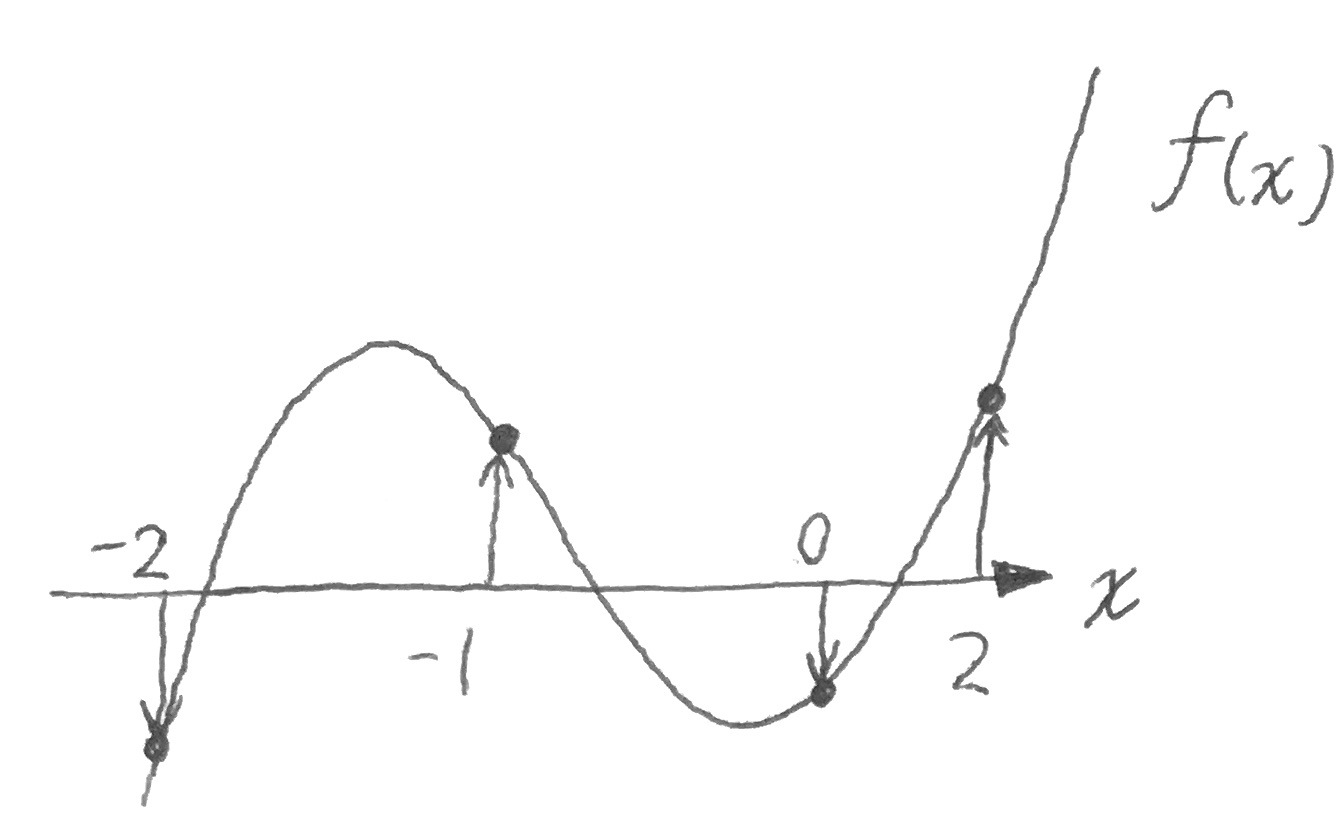
\includegraphics[width=5cm]{tuzi/image/0}
\end{figure}
\begin{flushright}
  $\square$
\end{flushright}

\noindent [3] 任意の解を$2\cos \theta$とすると、$\alpha = 2\cos \theta$とおける。$f(\alpha) = 0$より
\begin{align}
  \label{eq:toi1-1}
\alpha^3 + \alpha^2 -2\alpha -1 = 0
\end{align}
2倍角、3倍角の公式より
\begin{align}
2\cos 2\theta &= 4\cos^2 \theta -2 = \alpha^2 -2 \label{eq:toi1-2}\\
2\cos 3\theta &= \alpha^3 -3\alpha \label{eq:toi1-3}
\end{align}
ここで
\begin{eqnarray*}
  g(\alpha) &=& \frac{-1}{\alpha + 1}\\
  &=&\frac{\alpha^3 + \alpha^2 - 2\alpha -1}{\alpha + 1} \qquad\quad \text{(式(\ref{eq:toi1-1})より)}\\
  &=&\frac{\alpha^2(\alpha + 1) -2(\alpha + 1)}{\alpha + 1}\\
  &=&\alpha^2 -2\\
  &=&2 \cos 2\theta \qquad\qquad\qquad\quad\,\,\,\, \text{(式(\ref{eq:toi1-2})より)}
\end{eqnarray*}
また
\begin{eqnarray*}\hspace{20mm}
g(g(\alpha)) &=& -1 -\frac{1}{\alpha}\\
&=& \frac{(\alpha-1)(\alpha^3 + \alpha^2-2\alpha-1) -\alpha -1}{\alpha} \qquad \text{(式(\ref{eq:toi1-1})より)}\\
&=& \alpha^3 -3\alpha\\
&=& 2\cos 3\theta \hspace{50mm} \text{(式(\ref{eq:toi1-3})より)}
\end{eqnarray*}
よって$g(\alpha) = 2 \cos 2 \theta,\, g(g(\alpha)) = 2\cos 3\theta$となるので、$2\cos 2\theta,\, 2\cos 3\theta$は$f(x) = 0$の解である。
\begin{flushright}
  $\square$
\end{flushright}

\noindent [4] $2\cos \theta$ が$f(x) = 0$の解であるとき、[3]より$2\cos 2\theta$も解で、$2\cos 4\theta$も解である。
\begin{eqnarray*}
2\cos 2\theta &=& g(2 \cos \theta)\\
2\cos 3\theta &=& g(g(2\cos \theta))
\end{eqnarray*}
よって
\begin{eqnarray*}
2\cos 3 \theta = g(2\cos 2\theta)
\end{eqnarray*}
となるから
\begin{eqnarray*}
2\cos 4\theta &=& 2\cos 3\theta\\
\cos 4\theta &=& \cos 3\theta\\
4\theta &=& \pm 3 \theta + 2n\pi\ \ \ \text{($n$は整数)} \\
\end{eqnarray*}
$0<\theta<\pi$より
$$ \theta = \frac{2}{7}\pi,\,\frac{4}{7}\pi,\,\frac{6}{7}\pi $$
(つまり$f(x) = 0$の解は、$2\cos \frac{2}{7}\pi,\, 2\cos \frac{4}{7}\pi,\, 2\cos \frac{6}{7}\pi$ということ。)
\begin{flushright}
  $\square$
\end{flushright}

以下の問を用いてさらに考察していきましょう。

%
\section*{問2}
\addcontentsline{toc}{section}{問2}

\begin{screen}
問1の方程式$x^3+x^2-2x-1 =0$について$x =z + \frac{1}{z}$として、$z$の方程式であらわせ。さらに、その$z$の方程式を$h(z) = 0$として$(z-1)\cdot h(z) = 0$を解け。(解は$\cos,\, \sin,\, i$を用いてよい)
\end{screen}
%
\subsection*{解答}
\vspace{-10mm}
\begin{align*}
  & \left(z+\frac{1}{z}\right)^3+\left(z+\frac{1}{z}\right)^2-2\left(z+\frac{1}{z}\right)-1\\
  =& \,\, z^3+\frac{1}{z^3}+3z+\frac{3}{z}+z^2+\frac{1}{z^2} +2-2z -\frac{2}{z} -1\\
  =& \,\, z^3+z^2+z+1+\frac{1}{z} +\frac{1}{z^2}+\frac{1}{z^3} = 0
\end{align*}
両辺に$z^3(\neq 0)$をかけて
\begin{eqnarray*}
  z^6 + z^5 + z^4 + z^3 + z^2 +z + 1 = 0
\end{eqnarray*}
(なんと、$z$の相反方程式(しかも、すべての係数が1)が現れました。)\par
さらに
\begin{align*}\hspace{-30mm}
  (z-1)(z^6+z^5+z^4+z^3+z^2+z+1) &= 0\\
  z^7 -1 &= 0\\
  z^7 &= 1
\end{align*}
(zは1の7乗根ですね!)
$$ z = r(\cos \theta + i\sin \theta) \qquad (r>0,\, 0\leqq \theta < 2\pi) $$
とおくと
\begin{eqnarray*}
z^7 = r^7(\cos 7\theta + i\sin 7\theta)
\end{eqnarray*}
よって$z^7 = 1$は
\begin{eqnarray*}
r^7(\cos 7\theta + i\sin 7\theta) = \cos 0 + i\sin 0
\end{eqnarray*}
よって
$r^7 = 1$より$r=1$。\\
また、$7 \theta = 2n\pi \,\, (n = 0,1,2 \cdot \cdot \cdot ,6)$より$\theta = \frac{2n\pi}{7}$。\\
ゆえに$z_n = \cos\frac{2n\pi}{7} + i\sin\frac{2n\pi}{7}$\,\,($n = 0,1,\cdot \cdot \cdot,6$)と表せるから
\begin{align*}
  \begin{cases}
    \, z_0 = 1 \\
    \, z_1 = \cos\frac{2}{7}\pi + i\sin\frac{2}{7}\pi\\
    \, z_2 = \cos\frac{4}{7}\pi + i\sin\frac{4}{7}\pi\\
    \, z_3 = \cos\frac{6}{7}\pi + i\sin\frac{6}{7}\pi\\
    \, z_4 = \cos\frac{8}{7}\pi + i\sin\frac{8}{7}\pi\\
    \, z_5 = \cos\frac{10}{7}\pi + i\sin\frac{10}{7}\pi\\
    \, z_6 = \cos\frac{12}{7}\pi + i\sin\frac{12}{7}\pi
  \end{cases}
\end{align*}
\begin{flushright}
  $\square$
\end{flushright}

\vspace{10mm}
ここで、
$$x = z + \frac{1}{z} = z + \overline{z}$$
なので$z_1,z_2,z_3$を代入すると、それぞれ$2\cos \frac{2}{7}\pi,\, 2\cos\frac{4}{7}\pi,\, 2\cos\frac{6}{7}\pi$となり$f(x) = 0$の解になりますね。$z_4,z_5,z_6$を代入してもそれぞれ同じ値になりますね。
\begin{figure}[H]
  \centering
  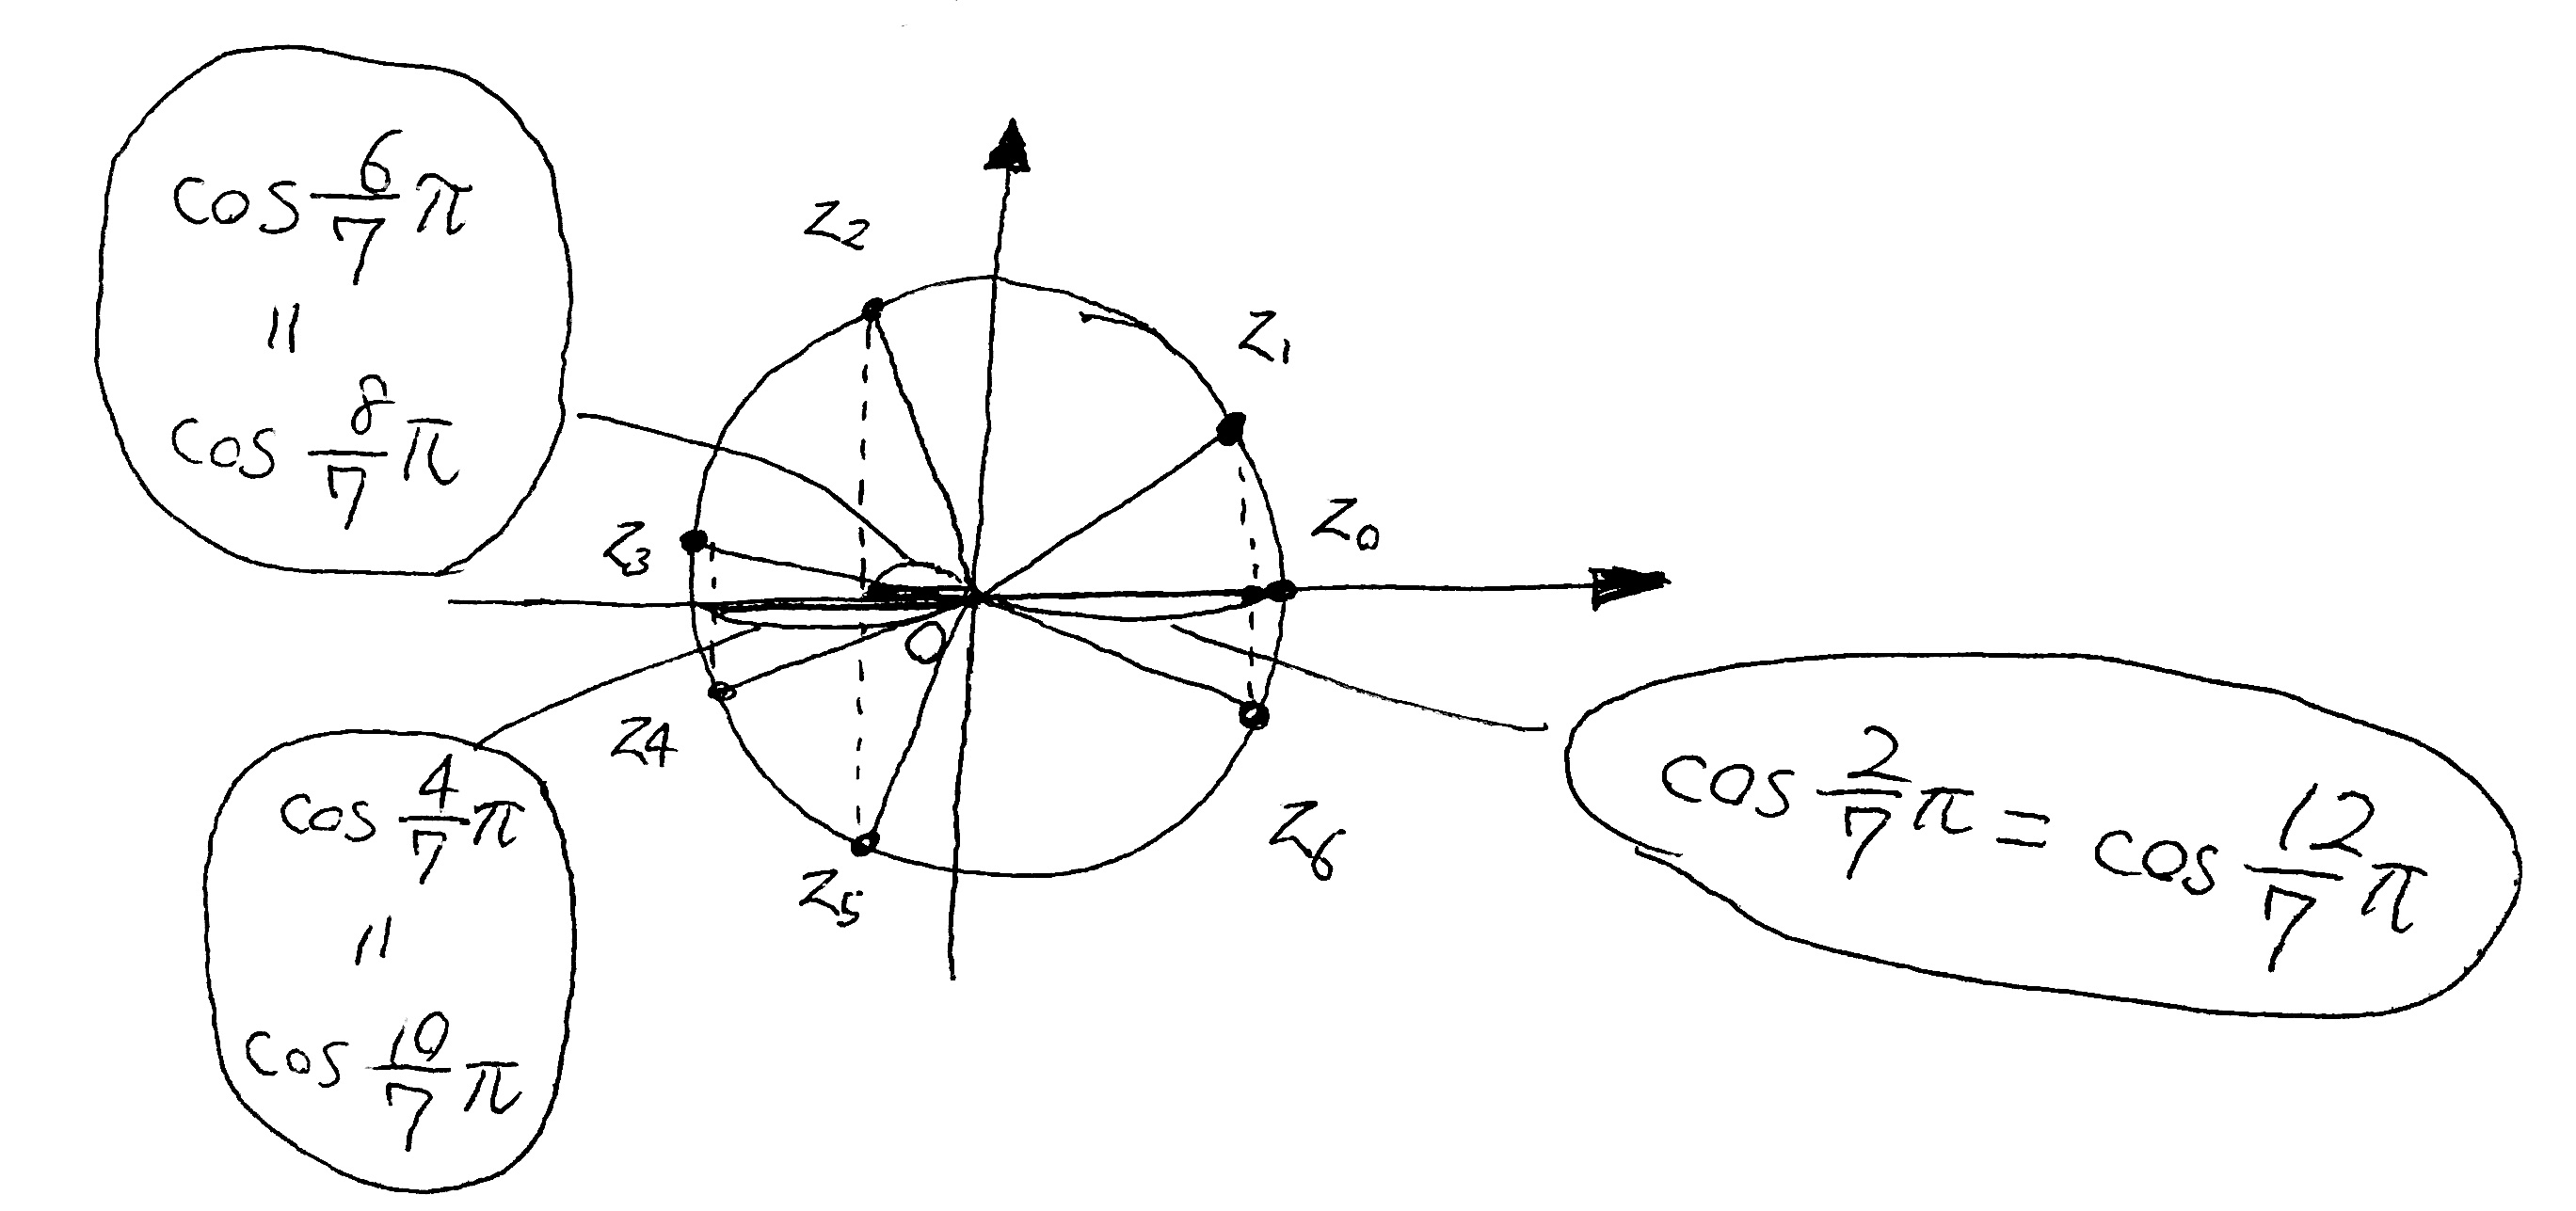
\includegraphics[width=10cm]{tuzi/image/1}
\end{figure}\par
似たような考え方で$\cos \frac{2}{5}\pi$の値を求めることができます。

%
\section*{問3}
\addcontentsline{toc}{section}{問3}
\begin{screen}
方程式$x^5 = 1$を用いて$\cos\frac{2}{5}\pi,\cos\frac{4}{5}\pi$の値を求めよ
\end{screen}
%
\subsection*{解答}
\begin{align*}
  x^5 &= 1\\
  x^5 -1 &= 0\\
  (x-1)(x^4+x^3+x^2+x+1) &= 0 \hspace{10zw}
\end{align*}
$x^4+x^3+x^2+x+1 = 0$について、$x \neq 0$より
$$
x^2 + x +1 + \frac{1}{x} + \frac{1}{x^2} = 0
$$
$t = x + \frac{1}{x}$とおくと
\begin{align*}
  t^2 -2 +t+1 &= 0\\
  t^2 + t - 1 &= 0
\end{align*}
よって
$$t = \frac{-1 \pm \sqrt{5}}{2}$$
また、$z = r(\cos \theta + i\sin \theta)$  ($r>0,\, 0\leqq \theta < 2\pi$)として
\begin{align*}
  r^5(\cos 5 \theta + i\sin 5 \theta) = \cos 0 + i\sin 0, \\
  r= 1,\quad \theta = \frac{2n\pi}{5}\,\,\,(n=0,1,2,3,4), \\
  x_n = \cos\frac{2n\pi}{5}+i\sin\frac{2n\pi}{5} \qquad
\end{align*}
よって
$$ t= x + \frac{1}{x} = 2\cos\frac {2n\pi}{5}$$
以上より
\begin{align*}
  \cos\frac{2}{5}\pi = \frac{\sqrt{5} - 1}{4}, \\
  \cos \frac{4}{5}\pi = -\frac{\sqrt{5} + 1}{4}
\end{align*}
\begin{flushright}
  $\square$
\end{flushright}

\begin{wrapfigure}{r}{40mm}
  \centering
  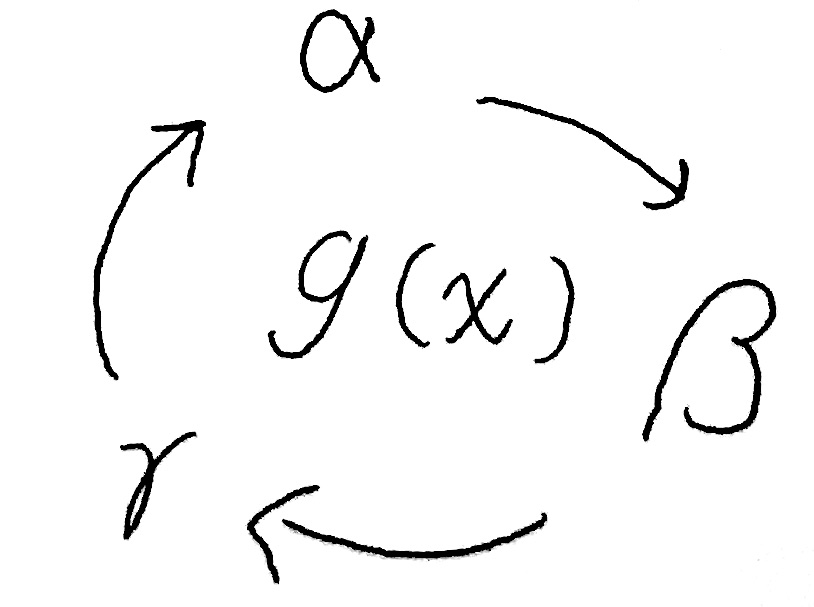
\includegraphics[width=25mm]{tuzi/image/2}
\end{wrapfigure}
問1で$f(x)$の解を$\alpha,\beta,\gamma$とすると、$g(x)$を用いて$\beta = g(\alpha),\gamma = g(\beta),\alpha = g(\gamma)$と循環しました。これについて考えてみましょう。


%
\section*{問4}
\addcontentsline{toc}{section}{問4}

\begin{screen}
  二次方程式$x^2+px+q = 0$の解$\alpha,\beta$(虚数解でもOKだが、重解は除く($\alpha \neq \beta$に矛盾))について$G(x) = ax +b$として、$G(\alpha) = \beta, G(\beta) = \alpha$が成立する$a,b$を求めよ。
\end{screen}
%
\subsection*{解答}
\begin{center}
  \begin{tabular}[t]{rl}
  \ldelim\{{2}{0pt}[]& \parbox[t]{5em}{
  $a\alpha+b=\beta$}\\
  & $a\beta+b=\alpha$
  \end{tabular}
\end{center}
2式から
$$a(\alpha -\beta)= \beta-\alpha$$
$\alpha \neq \beta$より
$$a = -1$$
このとき
\begin{align*}
  -(\alpha+\beta)+2b = \alpha + \beta \\
  b=\alpha+\beta
\end{align*}
よって、解と係数の関係より
$$\qquad b= -p$$
ゆえに
$$G(x) = -x-p$$
\begin{figure}[H]
  \centering
  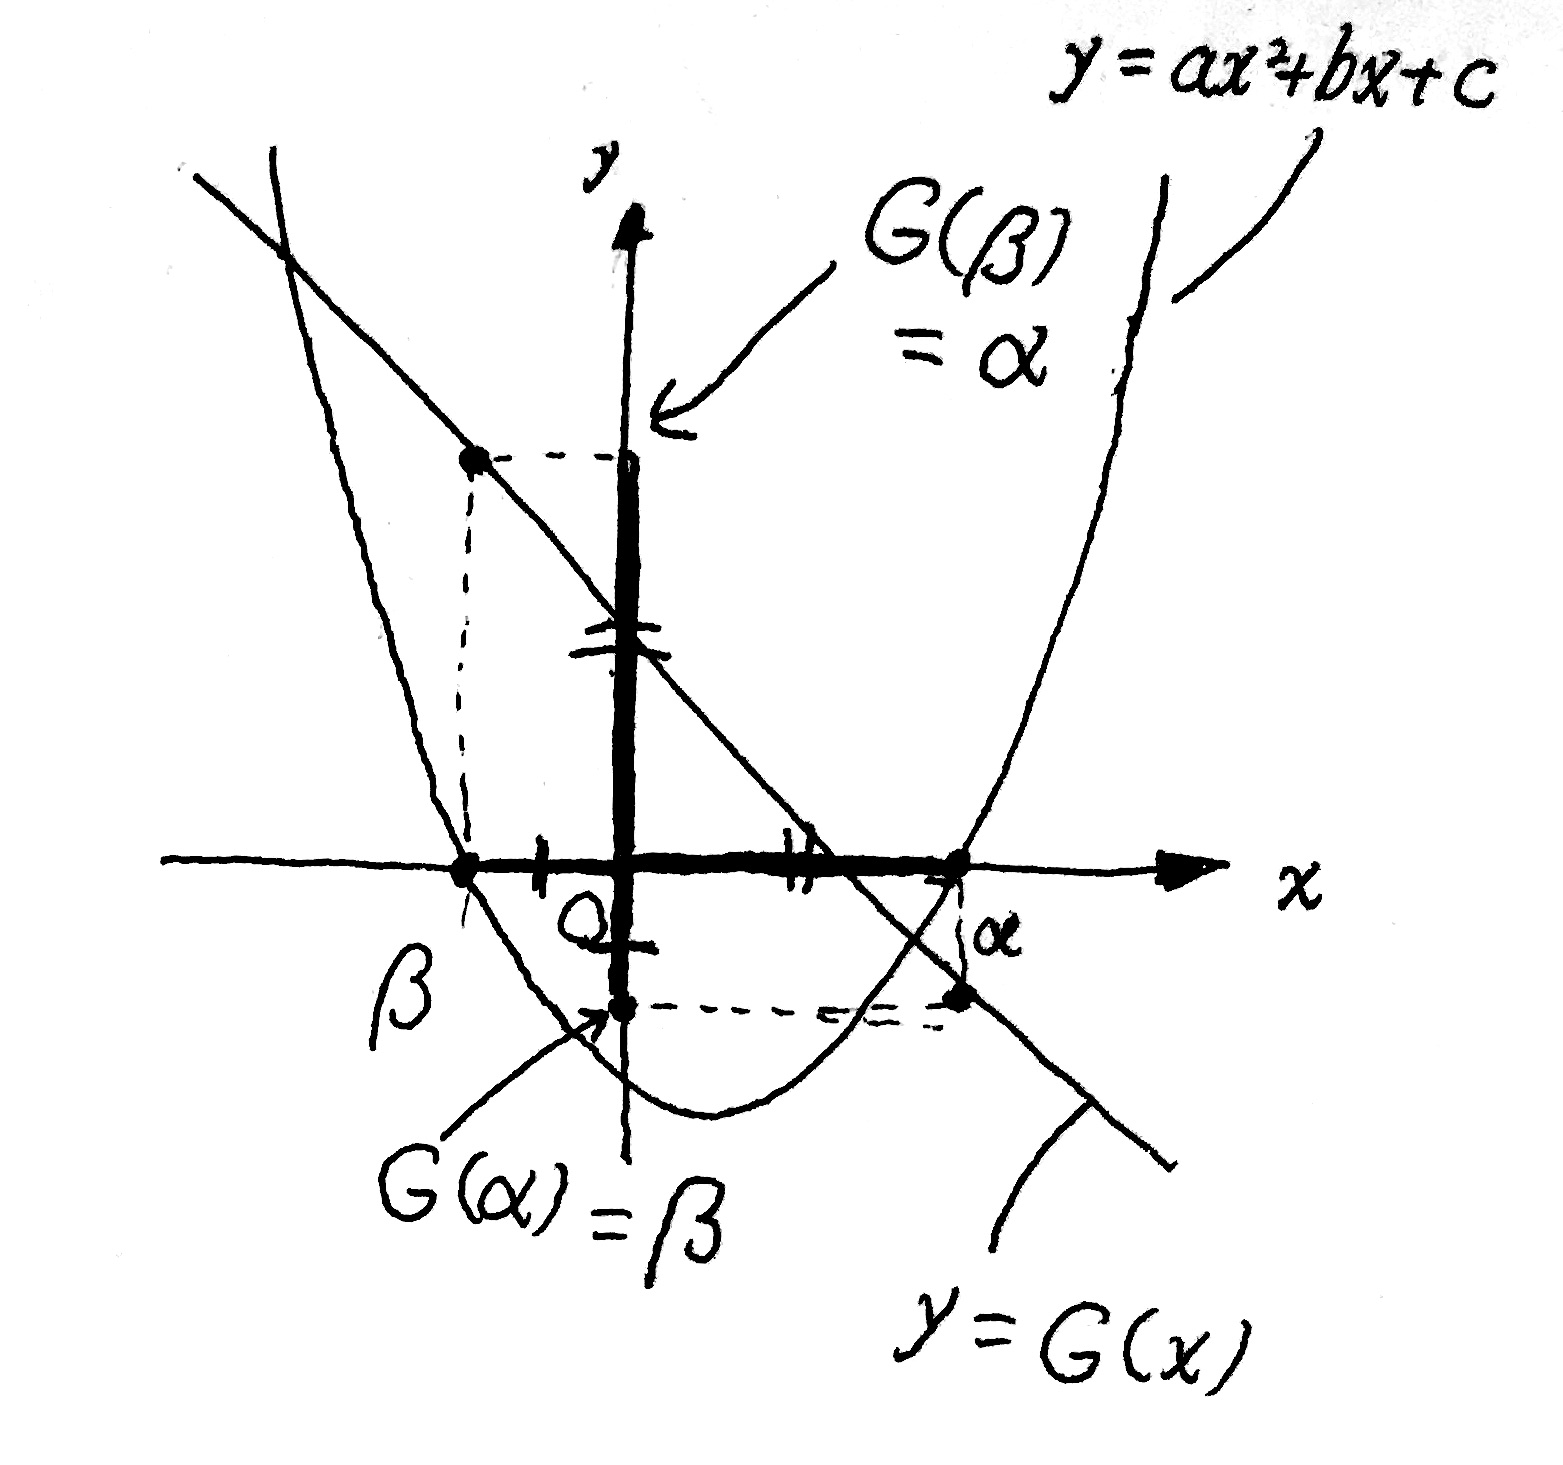
\includegraphics[width=6cm]{tuzi/image/4}
\end{figure}
\begin{flushright}
  $\square$
\end{flushright}

例えば$x^2+2x-8 = 0$について
$$G(x) = -x+2$$
となり解は$x = -2,4$なので
$$ G(-2) = -(-2)+2 = 4,\,\, G(4) = -4 +2 = -2 $$
と循環していますね。($G(G(-2)) = -2$)

\vspace{2zw}
\begin{itembox}[l]{\bf 二次方程式の解の循環}
  二次方程式$x^2+px+q = 0$の解の循環の式は$g(x) = -x -p$
\end{itembox}
\begin{itemize}
  \item 二次方程式の解の循環式では$g(g(x)) = x$が成り立ちます。
  \item 三次方程式の解の循環式はどうでしょう。導出は複雑すぎるので省きますが、解と係数の関係、判別式などを用いて連立すると導出できます。
\end{itemize}
\begin{itembox}[l]{\bf 三次方程式の解の循環}
三次方程式$x^3+px+qx+r = 0$の解の循環の式は$g(x) = ax^2+bx+c$。\\
ただし、
\begin{align*}
  s &= \pm \sqrt{p^2q^2-4p^3r-4q^3+18pqr-27r^2}\\
  & \hspace{40mm} \text{(ルートの中は判別式)}\\
  a &= \frac{3q-p^2}{s}\\
  b &= \frac{1}{2}\left(\frac{7pq-2p^3-qr}{s} - 1\right)\\
  c &= \frac{1}{2}\left(\frac{4q^2-p^2q-3pr}{s} - p\right)
\end{align*}
また
\begin{align*}
  x^3 + px+qx +r = g(x)h(x) +r \quad \text{($h(x)$は商、$r$は余り)}
\end{align*}
より$g(x)h(x) + r = 0$として\\
\[
g(x) = -\frac{r}{h(x)}
\]
より$-\frac{r}{h(x)} \quad \text{(一次分数関数)}$も解の循環式
\end{itembox}

これを用いて問1の$x^3+x^2-2x-1 = 0$の解の循環式は二次関数の形では
\[
g_1(x) = x^2 -2\ \ または\ \ g_2(x) = -x^2-x+1
\]
一次分数関数の形では
\[
g_1(x)よりh_1(x) =\frac{-1}{x+1}
\]
(問1と同じ循環式が出てきましたね)
\[
g_2(x)よりh_2(x)=-\frac{x+1}{x}
\]
$g_1(x),g_2(x),h_1(x),h_2(x)$の違いは何でしょうか。解$\alpha$を代入してみると
\begin{figure}[H]
  \centering
  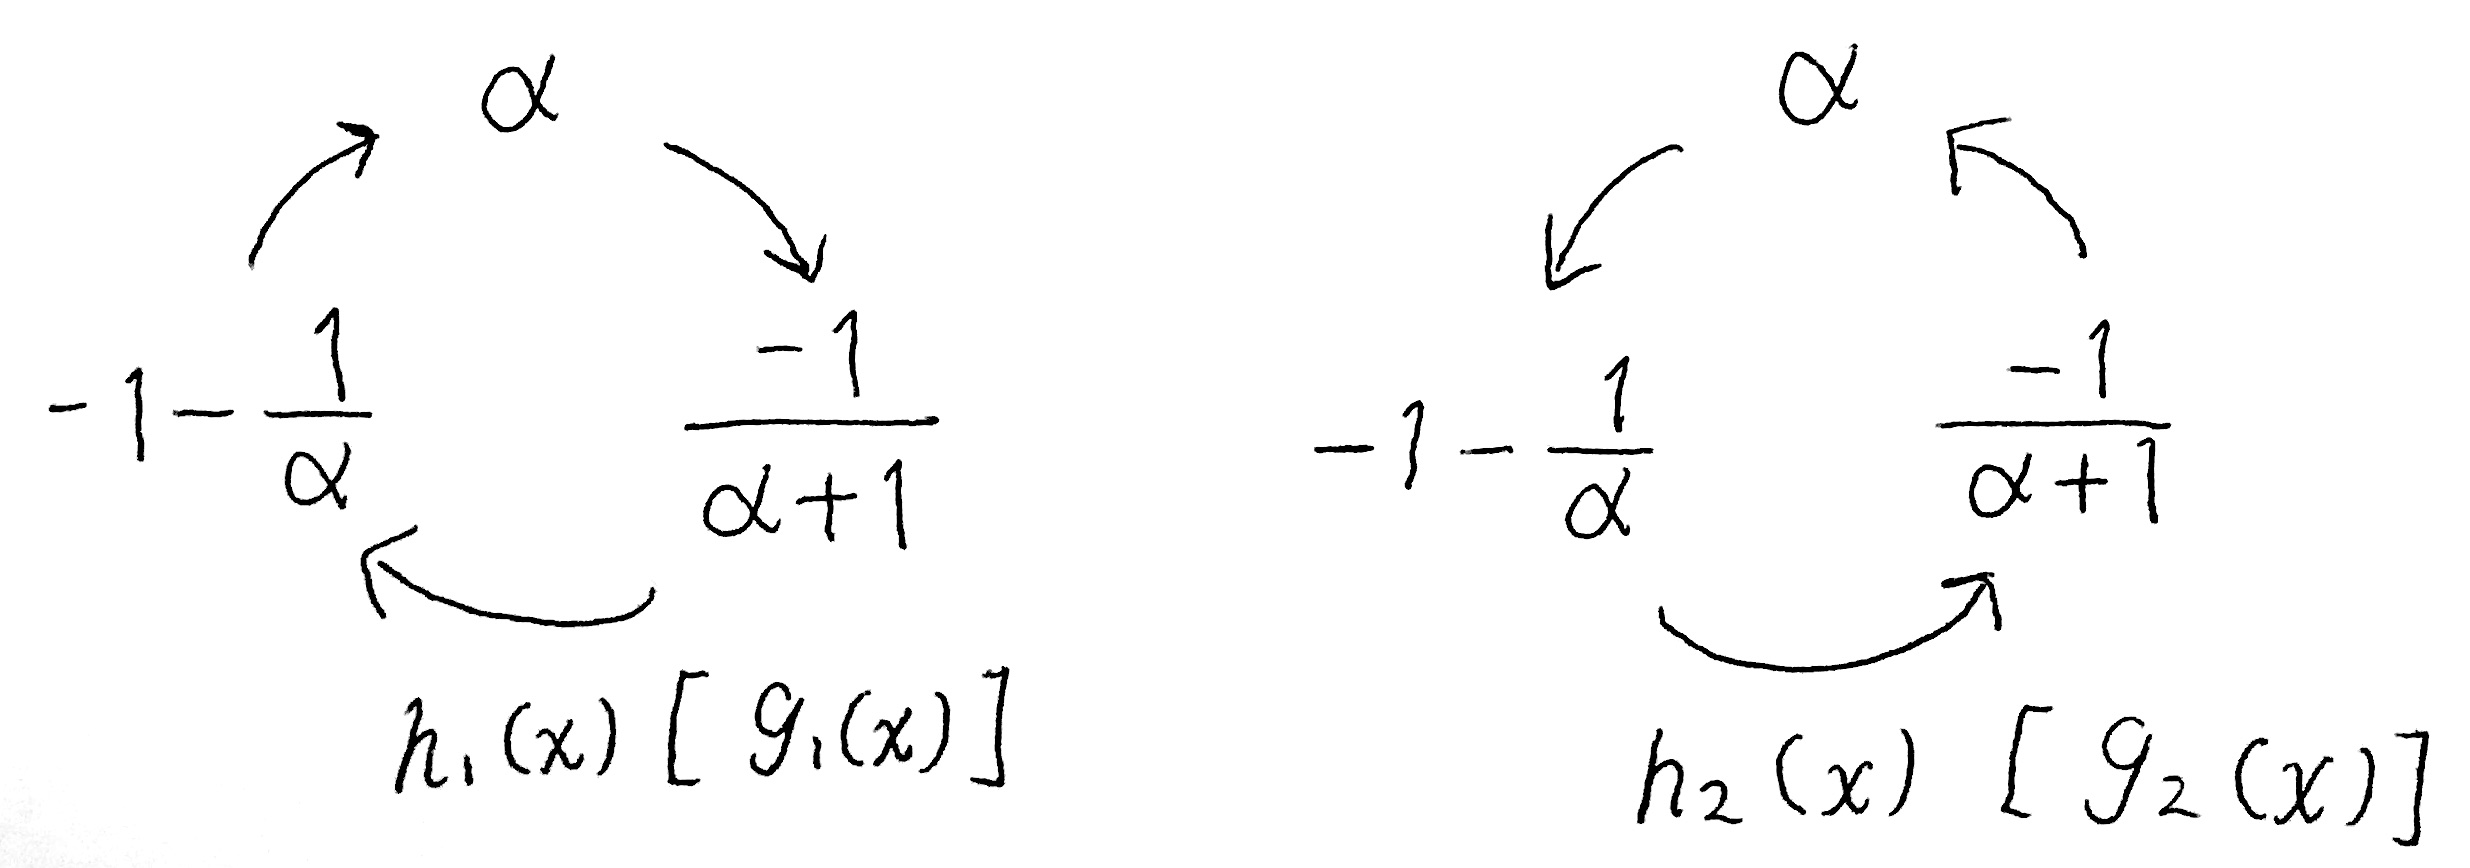
\includegraphics[width=7cm]{tuzi/image/5}
\end{figure}\noindent
と循環の方向が逆になります。\par
また、$g_1(g(g(x))) = x$ が成立するので
\begin{align*}
  \{(x^2-2)^2-2\}^2-2 = x\\
  x^8-8x^6+20x^4-16x^2-x+2 = 0
\end{align*}
よって
\[
(x^3+x^2-2x-1)(x^3-3x+1)(x+1)(x-2) = 0
\]
よって、$x^3-3x+1 = 0$は$g_1(x) = x^2-2$を循環式として持ちます。もう一つの循環式は$g_3(x)=-x^2-x+2$となり、一次分数関数の形では、それぞれ$h_3(x) = \frac{x-1}{x},h_4(x) = \frac{1}{1-x}$となります。$\alpha$を代入してみると
\begin{figure}[H]
  \centering
  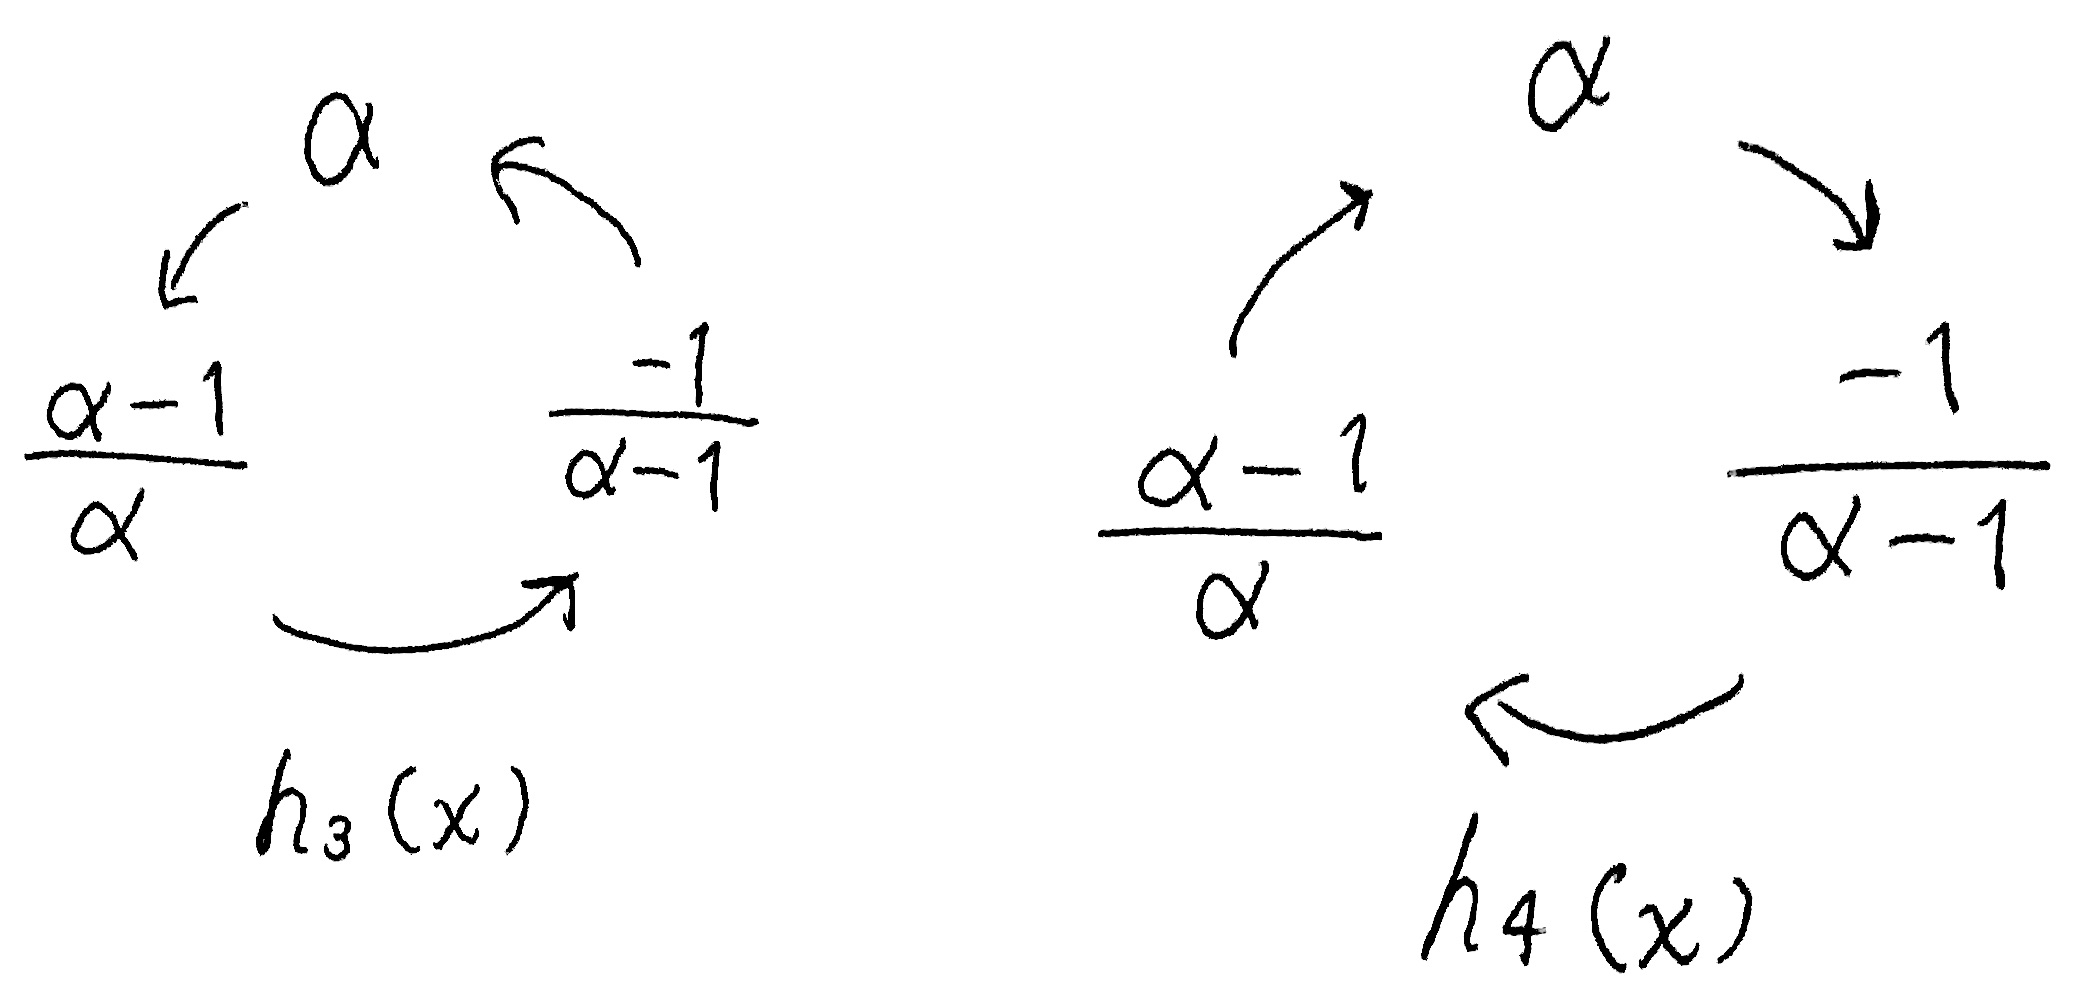
\includegraphics[width=7cm]{tuzi/image/6}
\end{figure}\noindent
となり循環しているのが確かめられました。\par
ちなみに$x+1 = 0,x-2=0$の解を$g_1(x)$に代入しても同じ解が得られます。

%
\section*{最後に一つ確認問題を}
\begin{screen}
  $x^3-6x^2+11x-6 = 0$の解と解の循環式を求め、循環することを確かめよ
\end{screen}
%
\subsection*{解答}\vspace{-3zw}
\begin{align*}
  & x= 1,2,3,\\
  & g_1(x)=-\frac{3}{2}x^2+\frac{11}{2}-2,\\
  & g_2(x) =\frac{3}{2}x^2-\frac{13}{2}x+8,\\
  & h_1(x)=\frac{10x-26}{6x-14},\\
  & h_2(x) = \frac{14x-26}{6x-10}
\end{align*}

\begin{figure}[H]
  \centering
  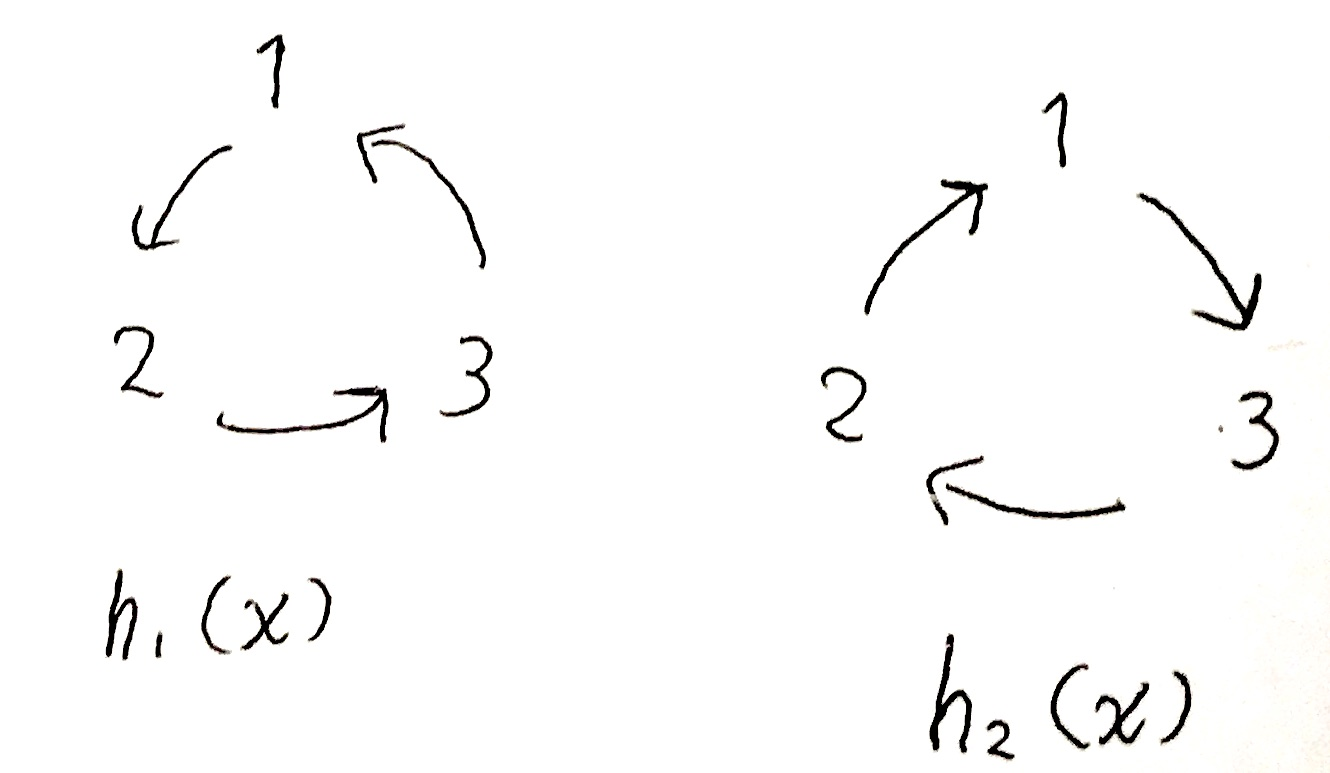
\includegraphics[width=6cm]{tuzi/image/7}
\end{figure}

%参考文献
%thebibliographyは使わないでください。\chapterになっちゃう!
\section*{参考文献}
\begin{enumerate}
  \item 解の巡回,\,「\url{http://www.004.upp.so-net.ne.jp/s_honma/solution/}\url{solution3.html}」
  \item 早稲田大学理工学部の入試問題
\end{enumerate}






%
 \clearpage
% 
% タイトル
\chapter{エントロピーの世界}
\vspace{-45pt} %高さ調整
\begin{flushright}
  {\bf \large 理工学部 物理科学科 2回生} \\ \vspace{3pt} %所属
  {\bf \large 西村 宗悟} \\ \vspace{30pt} %名前
\end{flushright}

% 序論
\section*{はじめに}
エントロピーという物理量が熱力学や統計力学で登場する。ここではエントロピーに対する考え方の初歩な話をする。最終的に熱力学の3法則の成立を理解することを目標とする。

%
\section{不可逆な変化}
\label{sec:hukagyaku}
%
\subsection{不可逆とは}
不可逆現象とは、逆向きの変化が起きない現象のことだ。例えばコップに水を入れて、そこにインクを一滴垂らしたとしよう。インクは水に触れると広がっていき、時間が経つと水全体を一様に染める。つまり、濃度が一様になるように拡散する。しかし、一度広がったインクは広がる前の一滴の雫の状態に自然に戻ることはない。つまり、覆水盆に返らずである。\par\begin{figure}[H]
  \centering
  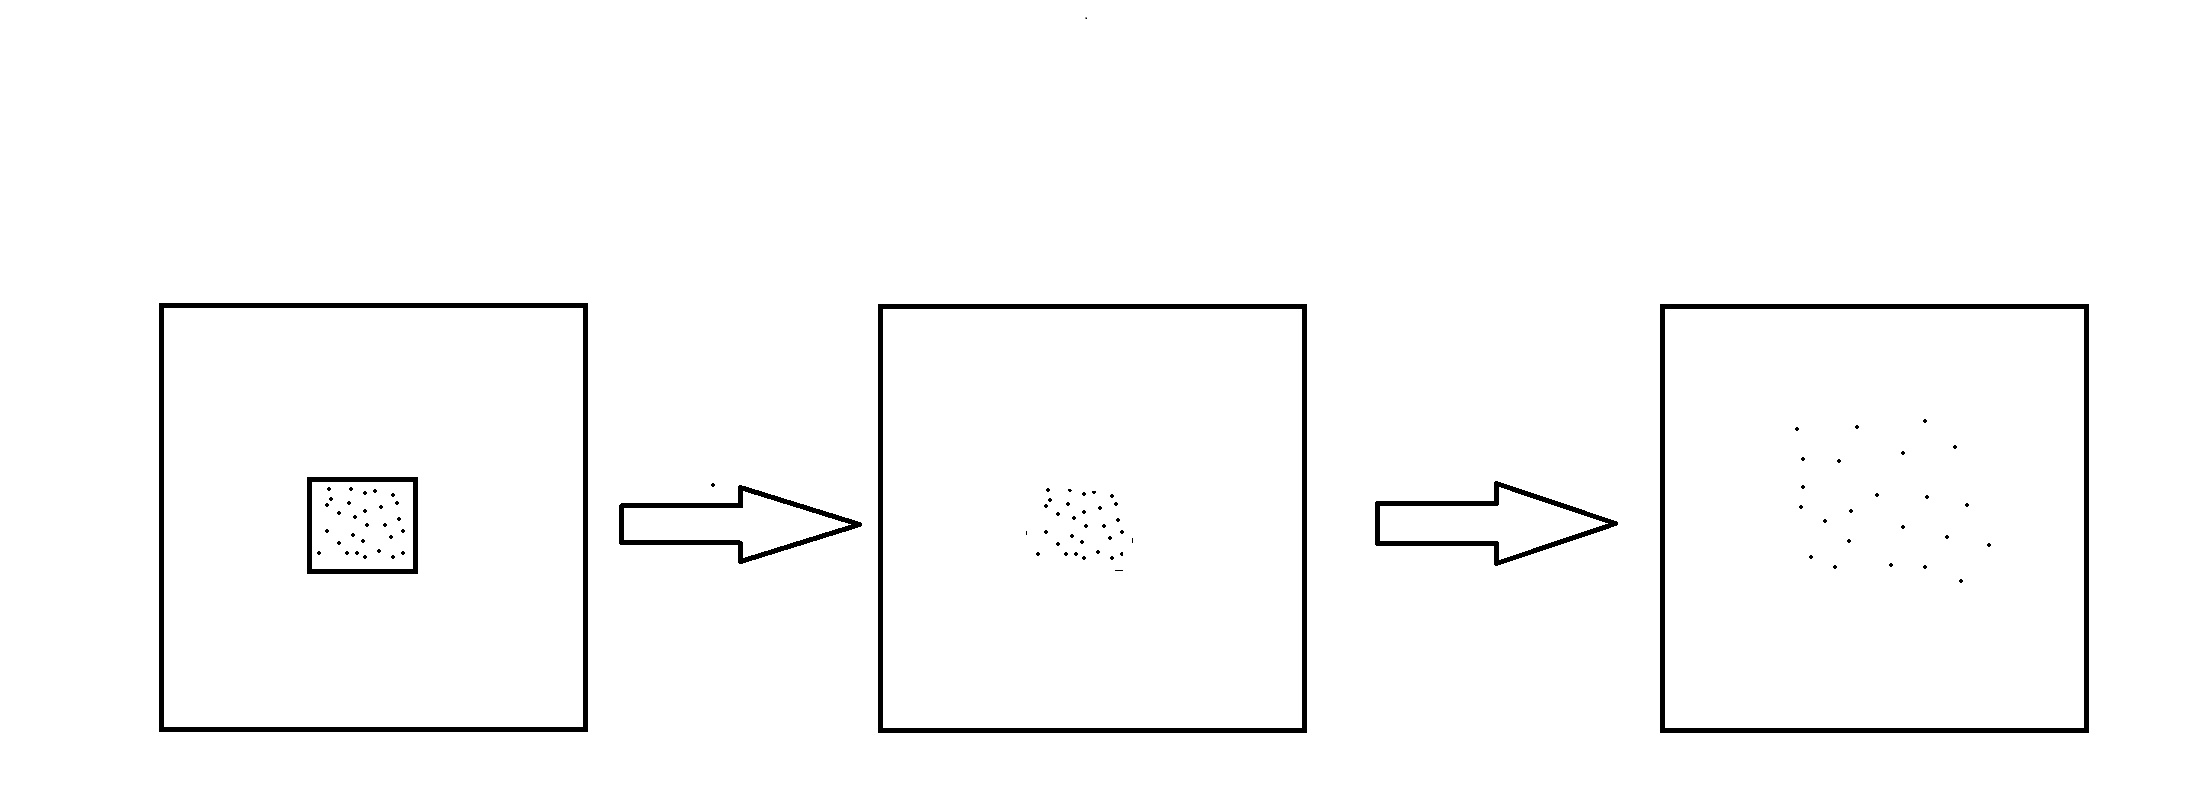
\includegraphics[width=10cm]{nishimura/image/2017112201.png}
  \caption{インクの広がりのイメージ図}
\end{figure}

「一度広がったインクは広がる状態の前に自然に戻ることはない」と断言したが、本当にそうなのかと疑問に思う人もいるだろう。それは不規則に運動するインクの分子が偶然、元の位置に戻ってくることがあってもいいのではないかという疑問だと思う。結論から言うと、そうなる確率がとても小さいので起こりにくいというのが答えだ。それを示すために気体分子を新しく例に挙げて考えてみよう。\par
大きな箱の中に小さな箱が入っており、小さな箱の中にN個の気体分子が入っているとしよう(図\ref{fig:V})。\begin{figure}[H]
  \centering
  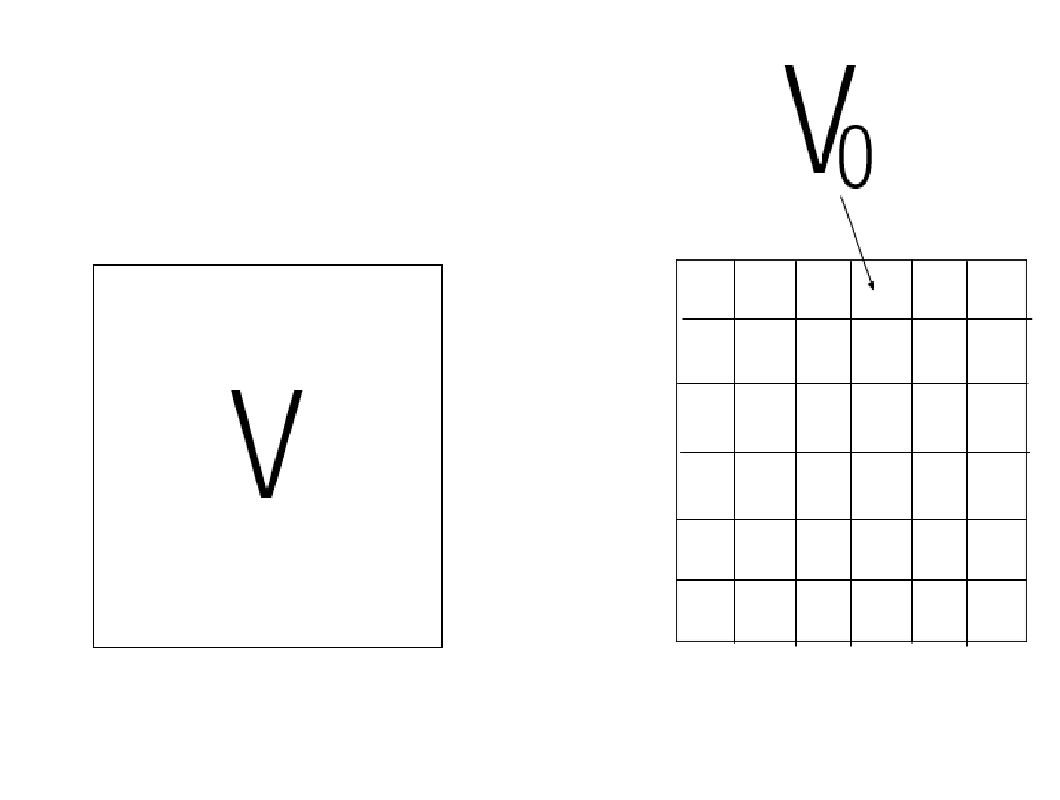
\includegraphics[width=10cm]{nishimura/image/2017112202.png}
  \caption{大きい箱と小さな箱の体積}
  \label{fig:V}
\end{figure}

大きな箱と小さな箱の体積比が$9:1$だとすると、$1$個の分子が小さな箱に入る確率は$1/10$だ。よって、$N$個の分子なら、一つ一つの分子が独立関係なので、$N$個の分子が全て小さな箱に入る確率$P$は
\begin{align}
 P=\left (\frac{1}{10}\right)^N \notag
\end{align}
になる。$1\mathrm{mol}$の気体で考えると$N=10^{23}$個とすれば、$P$がとても小さいことが分かる。経験的に部屋の空気がいきなり自然に部屋の隅に偏らないのはそうなる確率が低いからだ。もし、そんなことが起きれば部屋の中の人が窒息してしまう。\par
また、例に挙げたインクや気体分子が広がるというのは、広がる前よりも無秩序になったと言い換えることができる。まとめると自然に起こる変化はいつも無秩序さが増して、その変化は不可逆である。

%
\section{無秩序さとエントロピー}
\subsection{エントロピーとは}
\ref{sec:hukagyaku}で紹介した無秩序さについて、それを量的に捉えることを考える(エネルギーみたいに)。そこで登場するのがエントロピーだ。\par
体積Vの箱を用意し、それを体積の$V_0$微小領域に分割する(図\ref{fig:V})。分子がどれに入るかで分子の状態を表すとする。\ref{sec:hukagyaku}と同様に考えると、
\begin{align}
  \mathrm{1個の分子がとりうる状態の数} = \frac{V}{V_0}\\
	\mathrm{2個の分子がとりうる状態の数} = \left(\frac{V}{V_0}\right)^2\\
\mathrm{N個の分子がとりうる状態の数} = \left(\frac{V}{V_0}\right)^N \label{eq:W-N}
\end{align}
となる。$N$個の分子がとりうる状態の数を$W$とすると(\ref{eq:W-N})式より

\begin{align}
  \mathrm{W} =\left(\frac{V}{V_0}\right)^N  \label{itiyonn}
\end{align}
ここで、体積が$V_1$から$V_2$に変わった時の$W$の変化について考える。
\begin{align}
  \frac{W_2}{W_1}=\left(\frac{V_2}{V_1}\right)^N
\end{align}
無秩序さを表す量はエネルギーのように個数$N$に比例してほしい。だから、対数を用いてエントロピー$S$を定義する
\begin{align}
  S=k_B \ln{W} \label{eq:itiroku}
\end{align}
($k_B$:ボルツマン定数)\par
(\ref{eq:itiroku})の$W$に(\ref{itiyonn})を代入すると、
\begin{align}
  S=N k_B \ln{V}+定数  \label{snkb}
\end{align}
体積が$V_1$から$V_2$に変わったときのエントロピーが$S_1$から$S_2$になるとすれば、エントロピーの変化量は
\begin{align}
 \Delta S=S_2-S_1=N k_B \ln{\frac{V_2}{V_1}}  \label{itihati}
\end{align}
(\ref{itihati})より$V_2\textgreater V_1$なら$S_2\textgreater S_1$だから、体積か増加したらエントロピーが増加することがわかる。
\subsection{気体分子の速度の無秩序さ}
$速度空間で分子が分布している領域の体積\equiv \Omega$\\
$気体がその分子の速度についてとりうる状態の数\equiv W$\\
とすると、
\begin{align}
  W\propto \Omega^N   \label{itikyuu}
\end{align}
よって、エントロピーSは
\begin{align}
  S= N k_B \ln{\Omega}+定数
\end{align}
速度空間における、半径を$\overline{v}$,分子一個当たりのエネルギーを$\frac{E}{N}$とすると、
\begin{align}
  \frac{1}{2}m\overline{v}^2 &\simeq \frac{E}{N}\\
  \Rightarrow \overline{v} &\simeq \left(\frac{2E}{mN}\right)^{1/2}
\end{align}
したがって、領域の体積は
\begin{align}
  \Omega \simeq \frac{4}{3}\pi \overline{v}^3 \simeq \frac{4}{3}\pi \left(\frac{2E}{mN}\right)^{3/2}  \label{iisa}
\end{align}
これを(\ref{itikyuu})式に代入して、エネルギーに依存する部分だけを書くと、
\begin{align}
  W\propto \left(\frac{E}{N}\right)^{3N/2}   \label{iiyo}
\end{align}
(\ref{eq:itiroku})式に(\ref{iiyo})式を代入すると
\begin{align}
  S=\frac{3}{2}N k_B \ln{E}+定数   \label{iiro}
\end{align}
(\ref{iiro})式よりエネルギーが増加すると、エントロピーも増加することが分かる。
\section{気体の断熱変化}
断熱変化とは...エントロピーの増加をゼロとみなしていいような変化。\par
(\ref{iiro})式に気体の内部エネルギーと温度の関係
\begin{align}
  E=\frac{3}{2}N k_B \ln{T}
\end{align}
を代入すると、
\begin{align}
  S=\frac{3}{2}N k_B \ln{T} +定数   \label{itinana}
\end{align}
気体の断熱膨張を考えると、エントロピーは(\ref{snkb})式に従って増加するが、温度変化(減少)するので、(\ref{itinana})式に従って減少する。よって、
\begin{align}
  E&=Nk_B\ln{V}+\frac{3}{2}N k_B \ln{T}+定数\\
    &=Nk_B\ln VT^{3/2}+ 定数   \label{iiku}
\end{align}
$\Delta S=0の時にVT^{3/2}=一定となる。$

\section{秩序から無秩序へ}
ボルツマン分布よりエネルギー$E$のミクロな状態にある確率$P(E)$は
\begin{align}
  P(E)\propto\exp{(-E/{k_BT})}    \label{inio}
\end{align}
エネルギー$E$のミクロな状態の数$W$とすると、$W$個の状態一つ一つが(\ref{iiku})式によって実現する。\par
よって、マクロな状態にある確率$P'(E)$は
\begin{align}
   P'(E)\propto W\exp{(-E/{k_BT}) }   \label{inii}
\end{align}
(\ref{eq:itiroku})のエントロピーの定義より、
\begin{align}
   W=\exp{(S/k_B)}   \label{inini}
\end{align}
(\ref{inini})式を(\ref{inii})式に代入すると,
\begin{align}
   P'(E)\propto \exp{(-(E-TS)/{k_BT})}   \label{ijisa}
\end{align}
自由エネルギー$F$を
\begin{align}
   F\equiv E-TS    \label{Fteigi}
\end{align}
と定義する。\par
確率$P'(E)$が最大になるためには、$F$が最小になればよいので

\begin{align}
  \frac{dF}{dE}=1-T\frac{dS}{dE}=0\\
	\Rightarrow \frac{dS}{dE}=\frac{1}{T} \label{inigo}
\end{align}
温度一定で物体に$\Delta Q$の熱を加えたとすると、内部エネルギーは$\Delta E=\Delta Q$だけ増加する。\\
これを(\ref{inigo})式に使うと、エントロピーの変化量$\Delta S$は
\begin{align*}
  \Delta S=\frac{\Delta Q}{T}
\end{align*}
温度$T$と温度$\Delta Q$でエントロピーをあらわせた。
\section{熱力学の法則}
熱力学の第一法則\par
エネルギー保存則\par
\begin{align}
   Q=\Delta U +W
\end{align}
(加えた熱を$Q$、内部エネルギーの変化量を$\Delta U$、気体が外にした仕事を$W$とした。)\par
熱力学の第二法則\par
エントロピー増大測
\begin{align}
   \Delta S\geqq 0
\end{align}
($\Delta S$はエントロピーの増加量で等号成立は可逆過程の時)\par
熱力学の第三法則\\
\begin{align}
   `絶対零度では完全な秩序状態が実現する'
\end{align}
\ 第一法則と第二法則は経験則でわかる。系全体のエネルギーが保存するのは当たり前で、自然に起こる変化は乱雑になっていくことから、この二つは理解できる。\par
第三法則は何か難しいことを言っているように見えるが、ここまでの話から理解することができる。まず、温度が低いほどエントロピーは小さい((\ref{iiro})式より)。(\ref{Fteigi})式で$T=0$の時、$F=E$になる。絶対零度でエネルギーが最小なので、$F$も最小になる。$F$が最小ということは、マクロな状態にある確率$P'(E)$が最大で、確率は$1$になり、とりうる状態の数は一つに決まる。つまり、$T=0$で$W=1$。エントロピーの定義を考えると、$T→0$なら$S→0$になる。




%参考文献
%thebibliographyは使わないでください。\chapterになっちゃう!
\section*{参考文献}
\begin{enumerate}
  \item 長岡洋介・1997年・極低温の世界-超伝導への道-・岩波書店

\end{enumerate}





%
 \clearpage

% タイトル
\chapter{エントロピーの世界}
\vspace{-45pt} %高さ調整
\begin{flushright}
  {\bf \large 理工学部 物理科学科 2回生} \\ \vspace{3pt} %所属
  {\bf \large 西村 宗悟} \\ \vspace{30pt} %名前
\end{flushright}

% 序論
\section*{はじめに}
エントロピーという物理量が熱力学や統計力学で登場する。ここではエントロピーに対する考え方の初歩な話をする。最終的に熱力学の3法則の成立を理解することを目標とする。

%
\section{不可逆な変化}\label{sec:hukagyaku}
%
\subsection{不可逆とは}
不可逆現象とは、逆向きの変化が起きない現象のことだ。例えばコップに水を入れて、そこにインクを一滴垂らしたとしよう。インクは水に触れると広がっていき、時間が経つと水全体を一様に染める。つまり、濃度が一様になるように拡散する。しかし、一度広がったインクは広がる前の一滴の雫の状態に自然に戻ることはない。つまり、覆水盆に返らずである。\par\begin{figure}[H]
  \centering
  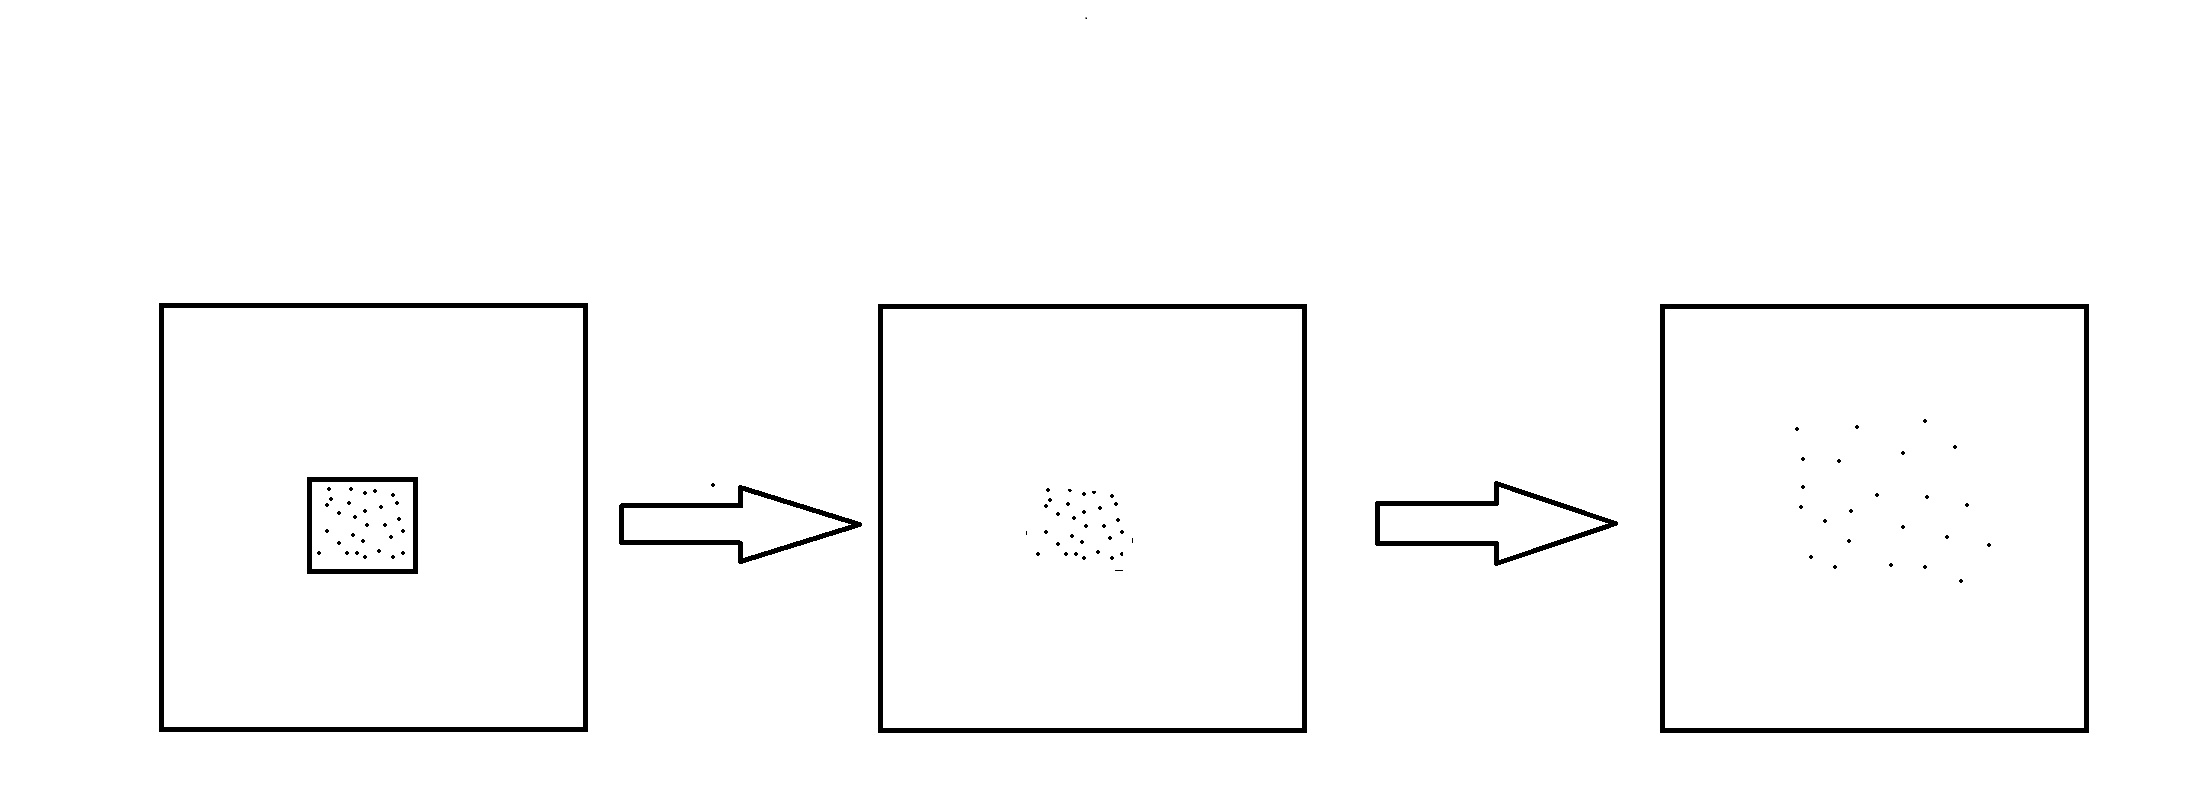
\includegraphics[width=10cm]{nishimura/image/2017112201.png}
  \caption{インクの広がりのイメージ図}
\end{figure}

「一度広がったインクは広がる状態の前に自然に戻ることはない」と断言したが、本当にそうなのかと疑問に思う人もいるだろう。それは不規則に運動するインクの分子が偶然、元の位置に戻ってくることがあってもいいのではないかという疑問だと思う。結論から言うと、そうなる確率がとても小さいので起こりにくいというのが答えだ。それを示すために気体分子を新しく例に挙げて考えてみよう。\par
大きな箱の中に小さな箱が入っており、小さな箱の中にN個の気体分子が入っているとしよう。\\

大きな箱と小さな箱の体積比が$9:1$だとすると、$1$個の分子が小さな箱に入る確率は$1/10$だ。よって、$N$個の分子なら、一つ一つの分子が独立関係なので、$N$個の分子が全て小さな箱に入る確率$P$は
\begin{align}
 P=\left (\frac{1}{10}\right)^N
\end{align}
になる。$1\mathrm{mol}$の気体で考えると$N=6.02×10^{23}$個とすれば、$P$がとても小さいことが分かる。経験的に部屋の空気がいきなり自然に部屋の隅に偏らないのはそうなる確率が低いからだ。もし、そんなことが起きれば部屋の中の人が窒息してしまう。\par
また、例に挙げたインクや気体分子が広がるというのは、広がる前よりも無秩序になったと言い換えることができる。まとめると自然に起こる変化はいつも無秩序さが増して、その変化は不可逆である。\newpage

%
\section{無秩序さとエントロピー}
\subsection{エントロピーとは}
セクション\ref{sec:hukagyaku}で紹介した無秩序さについて、それを量的に捉えることを考える(エネルギーみたいに)。そこで登場するのがエントロピーだ。\par

体積Vの箱を用意し、それを体積の$V_0$微小領域に分割する(図\ref{fig:V})。分子がどれに入るかで分子の状態を表すとする。セクション\ref{sec:hukagyaku}と同様に考えると、
\begin{align}
  \mathrm{1個の分子がとりうる状態の数} = \frac{V}{V_0}\\
	\mathrm{2個の分子がとりうる状態の数} = \left(\frac{V}{V_0}\right)^2\\
\mathrm{N個の分子がとりうる状態の数} = \left(\frac{V}{V_0}\right)^N \label{eq:W-N}
\end{align}
となる。$N$個の分子がとりうる状態の数を$W$とすると(\ref{eq:W-N})式より

\begin{align}
  \mathrm{W} =\left(\frac{V}{V_0}\right)^N  \label{itiyonn}
\end{align}
\begin{figure}[H]
  \centering
  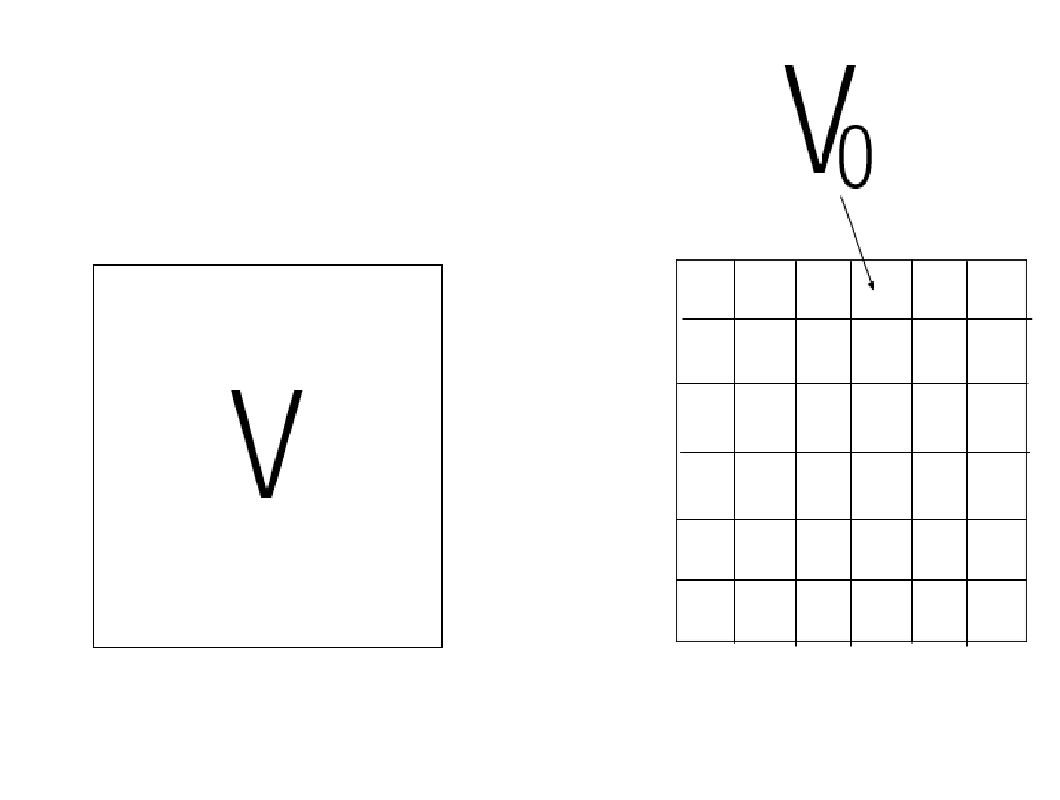
\includegraphics[width=10cm]{nishimura/image/2017112202.png}
  \caption{体積$V$の箱と体積$V_0$の微小領域}
  \label{fig:V}
\end{figure}
ここで、体積が$V_1$から$V_2$に変わった時の$W$の変化について考える。
\begin{align}
  \frac{W_2}{W_1}=\left(\frac{V_2}{V_1}\right)^N
\end{align}
無秩序さを表す量はエネルギーのように個数$N$に比例してほしい。だから、対数を用いてエントロピー$S$を定義する
\begin{align}
  S=k_B \ln{W} \label{eq:itiroku}
\end{align}
ここで、$k_B$はボルツマン定数と呼ばれていてボルツマン定数は$k_B=1.381×10^{23}[J\ K^{-1}]$である。\par
(\ref{eq:itiroku})の$W$に(\ref{itiyonn})を代入すると、
\begin{align}
  S=N k_B \ln{V}+定数  \label{snkb}
\end{align}
体積が$V_1$から$V_2$に変わったときのエントロピーが$S_1$から$S_2$になるとすれば、エントロピーの変化量は
\begin{align}
 \Delta S=S_2-S_1=N k_B \ln{\frac{V_2}{V_1}}  \label{itihati}
\end{align}
(\ref{itihati})より$V_2\textgreater V_1$なら$S_2\textgreater S_1$だから、体積が増加したらエントロピーが増加することがわかる。
\subsection{気体分子の速度の無秩序さ}
$速度空間で分子が分布している領域の体積\equiv \Omega$\\
$気体がその分子の速度についてとりうる状態の数\equiv W$\\
とすると、
\begin{align}
  W\propto \Omega^N   \label{itikyuu}
\end{align}
よって、エントロピーSは
\begin{align}
  S= N k_B \ln{\Omega}+定数
\end{align}
速度空間における、半径を$\overline{v}$,分子一個当たりのエネルギーを$\frac{E}{N}$とすると、
\begin{align}
  \frac{1}{2}m\overline{v}^2 &\simeq \frac{E}{N}\\
  \Rightarrow \overline{v} &\simeq \left(\frac{2E}{mN}\right)^{1/2}
\end{align}
したがって、領域の体積は
\begin{align}
  \Omega \simeq \frac{4}{3}\pi \overline{v}^3 \simeq \frac{4}{3}\pi \left(\frac{2E}{mN}\right)^{3/2}  \label{iisa}
\end{align}
これを(\ref{itikyuu})式に代入して、エネルギーに依存する部分だけを書くと、
\begin{align}
  W\propto \left(\frac{E}{N}\right)^{3N/2}   \label{iiyo}
\end{align}
(\ref{eq:itiroku})式に(\ref{iiyo})式を代入すると
\begin{align}
  S=\frac{3}{2}N k_B \ln{E}+定数   \label{iiro}
\end{align}
(\ref{iiro})式よりエネルギーが増加すると、エントロピーも増加することが分かる。
\section{気体の断熱変化}
断熱変化とは...エントロピーの増加をゼロとみなしていいような変化。\par
(\ref{iiro})式に気体の内部エネルギーと温度の関係
\begin{align}
  E=\frac{3}{2}N k_B \ln{T}
\end{align}
を代入すると、
\begin{align}
  S=\frac{3}{2}N k_B \ln{T} +定数   \label{itinana}
\end{align}
気体の断熱膨張を考えると、エントロピーは(\ref{snkb})式に従って増加するが、温度変化(減少)するので、(\ref{itinana})式に従って減少する。よって、
\begin{align}
  E&=Nk_B\ln{V}+\frac{3}{2}N k_B \ln{T}+定数\\
    &=Nk_B\ln VT^{3/2}+ 定数   \label{iiku}
\end{align}
$\Delta S=0の時にVT^{3/2}=一定となる。$

\section{秩序から無秩序へ}
統計力学によると温度$T$の環境の中に置かれた物体がエネルギー$E$の状態にある確率$P(E)$は
\begin{align}
  P(E)\propto\exp{(-E/{k_BT})}    \label{inio}
\end{align}
エネルギー$E$のミクロな状態の数$W$とすると、$W$個の状態一つ一つが(\ref{iiku})式によって実現する。\par
よって、マクロな状態にある確率$P'(E)$は
\begin{align}
   P'(E)\propto W\exp{(-E/{k_BT}) }   \label{inii}
\end{align}
(\ref{eq:itiroku})のエントロピーの定義より、
\begin{align}
   W=\exp{(S/k_B)}   \label{inini}
\end{align}
(\ref{inini})式を(\ref{inii})式に代入すると,
\begin{align}
   P'(E)\propto \exp{(-(E-TS)/{k_BT})}   \label{ijisa}
\end{align}
自由エネルギー$F$を
\begin{align}
   F\equiv E-TS    \label{Fteigi}
\end{align}
と定義する。\par
確率$P'(E)$が最大になるためには、$F$が最小になればよいので

\begin{align}
  \frac{dF}{dE}=1-T\frac{dS}{dE}=0\\
	\Rightarrow \frac{dS}{dE}=\frac{1}{T} \label{inigo}
\end{align}
温度一定で物体に$\Delta Q$の熱を加えたとすると、内部エネルギーは$\Delta E=\Delta Q$だけ増加する。\\
これを(\ref{inigo})式に使うと、エントロピーの変化量$\Delta S$は
\begin{align*}
  \Delta S=\frac{\Delta Q}{T}
\end{align*}
温度$T$と温度$\Delta Q$でエントロピーをあらわせた。
\section{熱力学の法則}
{\bf 熱力学の第一法則(エネルギー保存則)}\par
\begin{align}
   Q=\Delta U +W
\end{align}
(加えた熱を$Q$、内部エネルギーの変化量を$\Delta U$、気体が外にした仕事を$W$とした。)\par
{\bf 熱力学の第二法則(エントロピー増大測)}
\begin{align}
   \Delta S\geqq 0
\end{align}
($\Delta S$はエントロピーの増加量で等号成立は可逆過程の時)\par
{\bf 熱力学の第三法則}\\
\begin{align}
   `絶対零度では完全な秩序状態が実現する'
\end{align}
\ 第一法則と第二法則は経験則でわかる。系全体のエネルギーが保存するのは当たり前で、自然に起こる変化は乱雑になっていくことから、この二つは理解できる。\par
第三法則は何か難しいことを言っているように見えるが、ここまでの話から理解することができる。まず、温度が低いほどエントロピーは小さい((\ref{iiro})式より)。(\ref{Fteigi})式で$T=0$の時、$F=E$になる。絶対零度でエネルギーが最小なので、$F$も最小になる。$F$が最小ということは、マクロな状態にある確率$P'(E)$が最大で、確率は$1$になり、とりうる状態の数は一つに決まる。つまり、$T=0$で$W=1$。エントロピーの定義を考えると、$T→0$なら$S→0$になる。




%参考文献
%thebibliographyは使わないでください。\chapterになっちゃう!
\section*{参考文献}
\begin{enumerate}
  \item 長岡洋介、1997年、極低温の世界-超伝導への道-、岩波書店
 \item Sinshu Univ.Physical Chemistry Lab.Adsorption Group、定数について、「\url{science.shinshu-u.ac.jp/~tiiyama/?page_id=1564}」
\end{enumerate}





%
 \clearpage
% タイトル
\chapter{線の形}
\vspace{-45pt} %高さ調整
\begin{flushright}
  {\bf \large 理工学部 物理科学科 2回生} \\ \vspace{3pt} %所属
  {\bf \large 中山 敦貴} \\ \vspace{30pt} %名前
\end{flushright}


%
\section*{はじめに}
去年の会誌ではサインカーブとカテナリー曲線の話をした。今回もそれの続きとしてまた曲線の話である。メインは最速降下曲線の話であるが、これは去年の会誌でやるつもりだったが、なかなか手強くて今回リベンジすることになった。ついでにインボリュート曲線とトラクトリックスという曲線についても考えた。これらについてはただ計算をガリガリしたかっただけである。

%%%%%%%%%%%%%%%%%%%%%%%%%%%%%%%%%%%%%%%%%%%%%%%%%%%%
\section{インボリュート曲線}
%%%%%%%%%%%%%%%%%%%%%%%%%%%%%%%%%%%%%%%%%%%%%%%%%%%%

\subsection{インボリュート曲線とは}
\begin{wrapfigure}{r}{40mm}
  \centering
  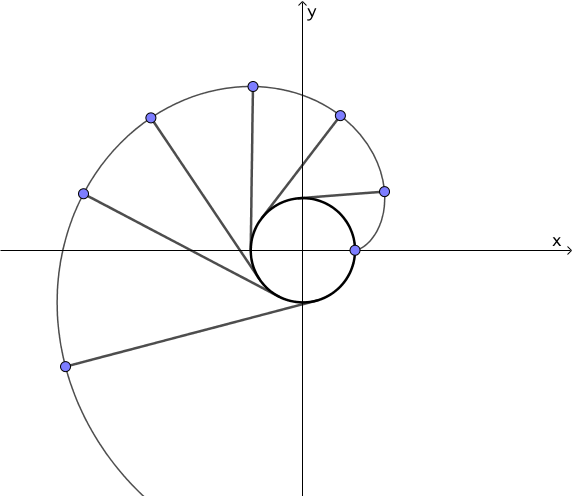
\includegraphics[width = 6cm]{nakayama1/image/imbo3}
\end{wrapfigure}
円形の筒に糸が巻かれている。その糸をピンと張りながらほどいていくとき、糸の端点が描く軌道をインボリュート曲線と呼ぶ。

\subsection{曲線の式}
それでは早速、この曲線の式を求めてみよう。半径$a$の円筒に糸が巻きつけられているとして、その糸をピンと張りながらどんどんほどいていくときを考える。

\begin{figure}[H]
  \centering
  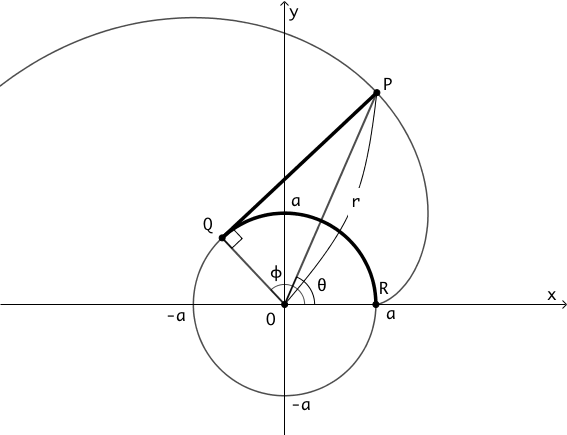
\includegraphics[width=8cm]{nakayama1/image/imbo1}
\end{figure}

円弧$\ko{QR}$の長さは、ほどいた糸$\mathrm{PQ}$の長さに等しいので
\begin{align*}
  \ko{QR} = 2\pi a \times \frac{\phi}{2\pi} = a\phi = \mathrm{PQ}
\end{align*}
となる。
よって$\triangle \mathrm{OPQ}$で次のことが言える。
\begin{spacing}{0.2}
\end{spacing}
  \begin{align*}
    \sin(\phi - \theta) &= \frac{a\phi}{r} \qquad\qquad \text{$\mathrm{PQ} = a\phi$だから}\\
    \sin\phi \cos\theta - \cos\phi \sin\theta &= \frac{a\phi}{r} \qquad\qquad \text{左辺を加法定理でバラした}\\
    r\cos\theta \sin\phi - r\sin\theta \cos\phi &= a\phi \qquad\qquad \text{両辺に$r$をかけた}\\
    x\sin\phi - y\cos\phi &= a\phi \qquad\qquad \text{直交座標に直した}
  \end{align*}
また、同様にして
\begin{spacing}{1}
  \begin{align*}
    \cos(\phi - \theta) &= \frac{a}{r}\\
    \cos\phi \cos\theta + \sin\phi \sin\theta &= \frac{a}{r} \qquad\qquad \text{左辺を加法定理でバラした}\\
    r\cos\theta \cos\phi + r\sin\theta \sin\phi &= a \qquad\qquad \text{両辺に$r$をかけた}\\
    x\cos\phi + y\sin\phi &= a \qquad\qquad \text{直交座標に直した}
  \end{align*}
\end{spacing}\noindent
よって、$x$と$y$についての式が2つ得られた
\begin{align*}
  \begin{cases}
  \,\cos\phi \cos\theta + \sin\phi \sin\theta = \dfrac{a}{r}\\
  \,x\cos\phi + y\sin\phi = a
  \end{cases}
\end{align*}
あとはこの連立方程式を解けばいいのだが、せっかくなので線形代数の力を借りて美しく解いてみようと思う。\par
まずは2式を行列を使って表す。
\begin{align*}
  \begin{pmatrix}
    \sin\phi & -\cos\phi \\
    \cos\phi & \sin\phi \\
  \end{pmatrix}
  \begin{pmatrix}
    x\\y\\
  \end{pmatrix}
  =
  \begin{pmatrix}
    a\phi\\a\\
  \end{pmatrix}
\end{align*}
行列式を計算すると
\begin{align*}
  \begin{vmatrix}
    \sin\phi & -\cos\phi \\
    \cos\phi & \sin\phi \\
  \end{vmatrix}
  =\sin^2\phi + \cos^2\phi = 1
\end{align*}
であるから、クラーメルの公式より
  \begin{align*}
    x &=
    \begin{vmatrix}
      a\phi & -\cos\phi \\
      a & \sin\phi \\
    \end{vmatrix}
    = a(\cos\phi + \phi\sin\phi)\\
    y &=
    \begin{vmatrix}
      \sin\phi & a\phi \\
      \cos\phi & a \\
    \end{vmatrix}
    = a(\sin\phi - \phi\cos\phi)
  \end{align*}
よってインボリュート曲線は
\begin{align*}
  \begin{cases}
  \,x = a(\cos\phi + \phi\sin\phi)\\
  \,y = a(\sin\phi - \phi\cos\phi)
  \end{cases}
\end{align*}
とパラメータ表示できることがわかった。

\begin{figure}[H]
  \centering
  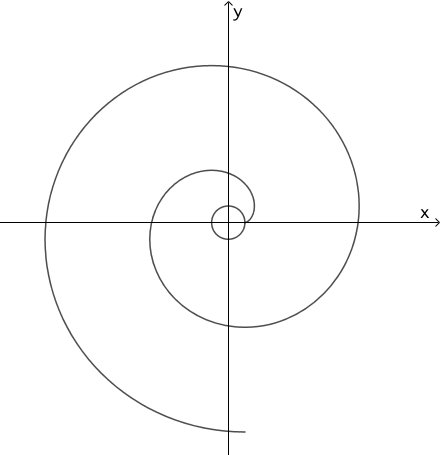
\includegraphics[width=8cm]{nakayama1/image/imbo2}\\
  $0 \le \phi \le 4\pi$におけるインボリュート曲線
\end{figure}

\subsection{伸開線}
  一般に、ある曲線に巻きつけられた糸を弛まないように引っ張りつつほどいていくときの、糸の端点が描く軌道を伸開線という。円の伸開線はさっき求めたインボリュート曲線である。前回の会誌で考えたカテナリー曲線の伸開線は、次節で紹介するトラクトリックスになっている。暇な人は考えてみよう。伸開線のWikipediaにわかりやすいGIFがあるので見てみるとよい。


%%%%%%%%%%%%%%%%%%%%%%%%%%%%%%%%%%%%%%%%%%%%%%%%%%%%
\section{トラクトリックス}
%%%%%%%%%%%%%%%%%%%%%%%%%%%%%%%%%%%%%%%%%%%%%%%%%%%%

\subsection{トラクトリックスとは}
石ころに紐を結び、図のように$x$軸に沿って紐を引くとき、石ころが描く軌道をトラクトリックスまたは牽引曲線と呼ぶ。
また、各点での接線と$x$軸との間の長さが一定であるような曲線であるとも言える。\par
\begin{figure}[H]
  \centering
  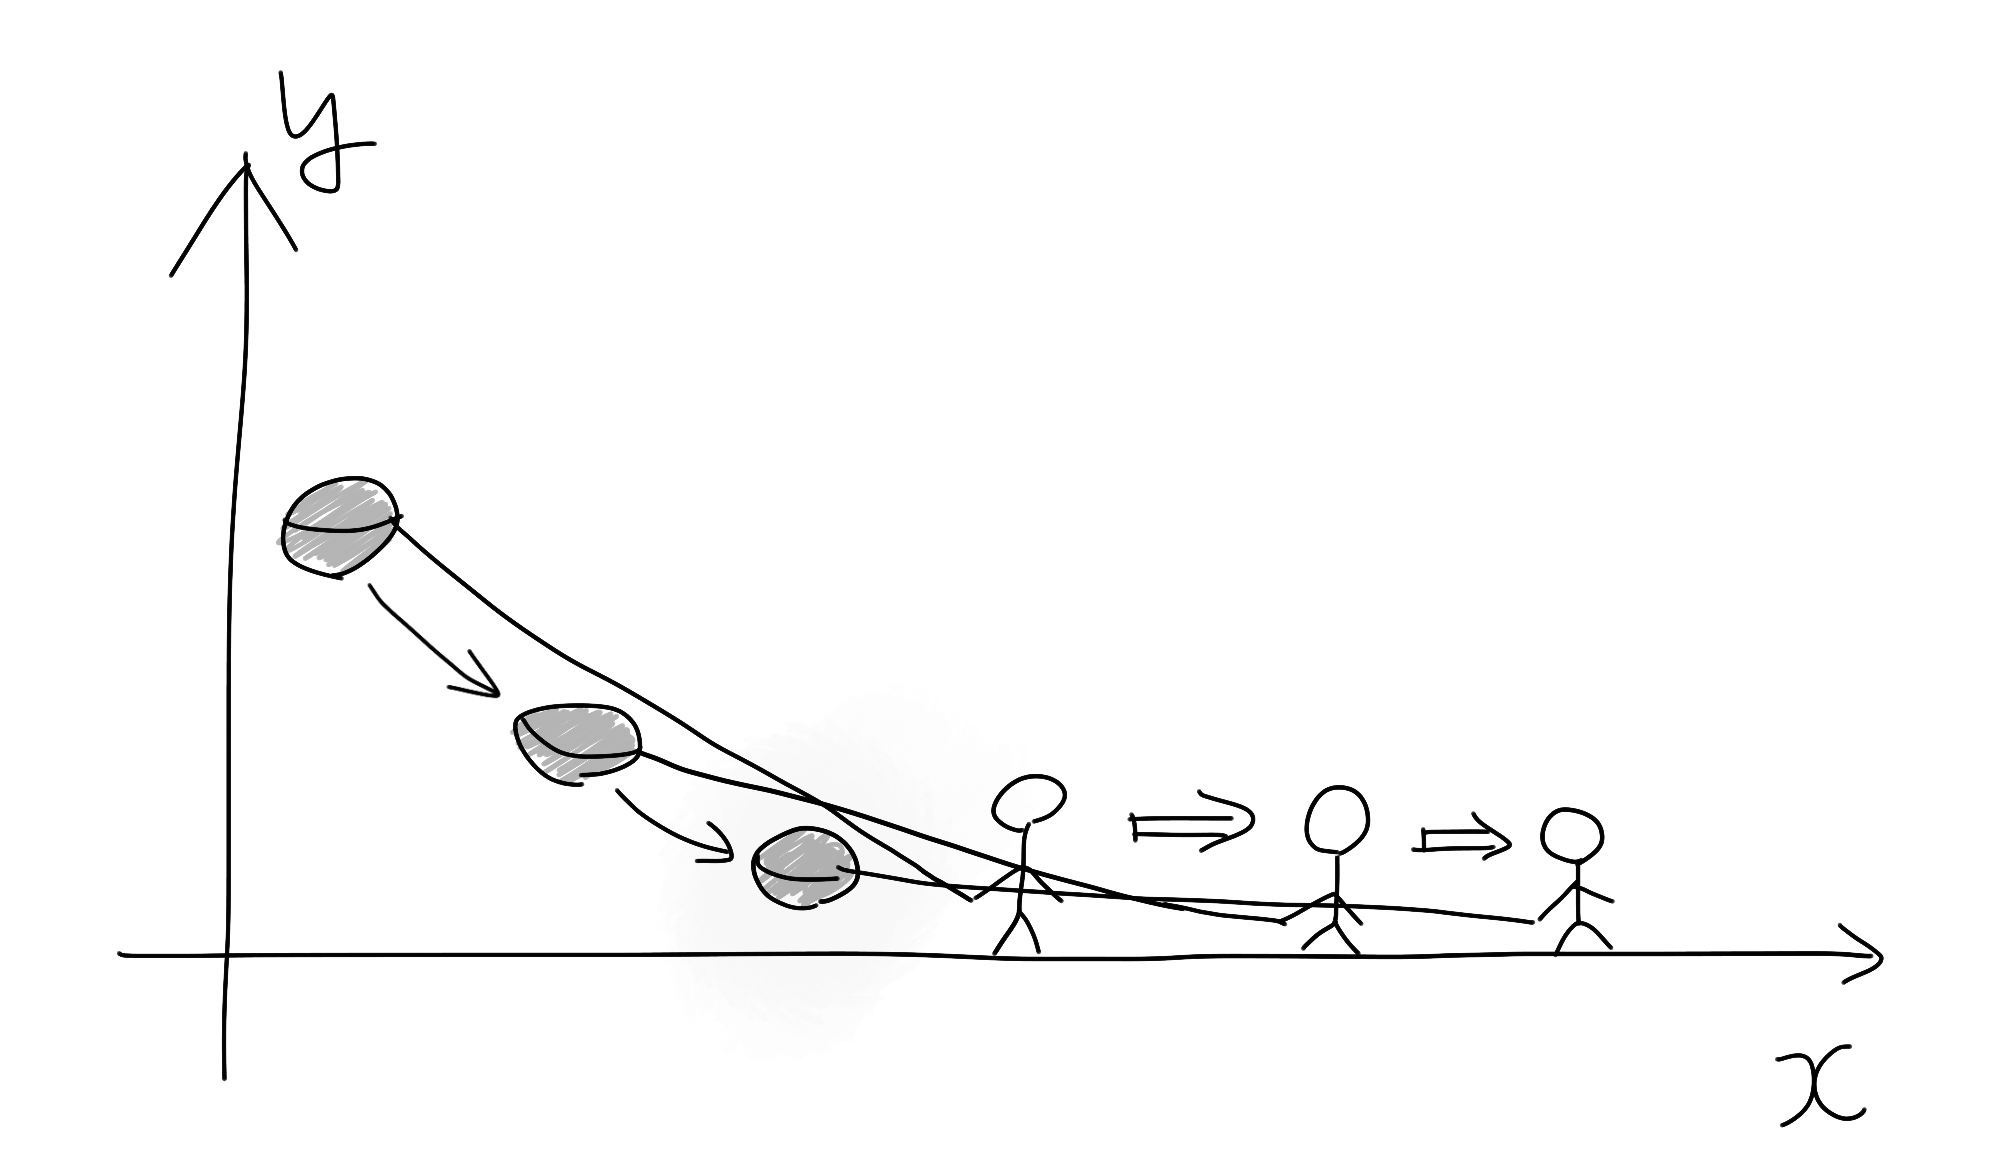
\includegraphics[width=8cm]{nakayama1/image/trac1}\\
  {\small トラクトリックスが描かれていく様子}
\end{figure}

\subsection{曲線の式}

初めの石ころの位置を$(0,a)$、引っ張る人の位置を原点$(0,0)$とする。ここから引っ張る人は$x$軸上を右に進んでいく。\par
石ころに力を伝えるのは紐であるから、紐は常に作用線上にある。作用線は曲線の導関数に一致するので、紐は接線上にあることになる。

\begin{figure}[H]
  \centering
  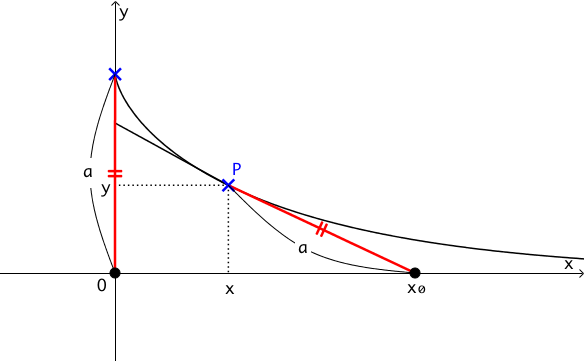
\includegraphics[width=8cm]{nakayama1/image/trac2}
\end{figure}

三平方の定理より
\begin{align*}
  y^2 + (x_0 - x)^2 &= a^2 \\
  (x_0 - x)^2 &= a^2 - y^2
\end{align*}
$x < x_0$であるから
\begin{align*}
  x_0 - x &= \sqrt{a^2 - y^2}
\end{align*}
よって、接線の傾きを考えると
\begin{align*}
  \frac{\mathrm{d}y}{\mathrm{d}x} = - \frac{y}{x_0 - x} = - \frac{y}{\sqrt{a^2 - y^2}}
\end{align*}
が成り立つことがわかる。あとはこの微分方程式を$x$について解いていく。\par
まずは変数を分離して両辺積分する。
\begin{align*}
  \mathrm{d}x &= - \frac{\sqrt{a^2 - y^2}}{y} \,\mathrm{d}y \\
  \int \mathrm{d}x &= - \int \frac{\sqrt{a^2 - y^2}}{y} \,\mathrm{d}y \\
  x &= - \int \frac{\sqrt{a^2 - y^2}}{y} \,\mathrm{d}y
\end{align*}
右辺は置換積分で計算する。$u = \sqrt{a^2 - y^2}$とおくと、$0 < y$であるから
\begin{align*}
  y = \sqrt{a^2 - u^2}
\end{align*}
よって
\begin{align*}
  \frac{\mathrm{d}y}{\mathrm{d}u} = - \frac{u}{\sqrt{a^2 - u^2}}
\end{align*}
であるから、これらで置換して
\begin{align*}
  x &= - \int \frac{u}{\sqrt{a^2 - u^2}} \cdot \left(- \frac{u}{\sqrt{a^2 - u^2}}\right) \,\mathrm{d}u \\
  &= \int \frac{u^2}{a^2 - u^2} \,\,\mathrm{d}u
\end{align*}
少し変形すると
\begin{align*}
  x &= - \int \frac{u^2}{u^2 - a^2} \,\,\mathrm{d}u \\
  &= - \int \frac{u^2 - a^2 + a^2}{u^2 - a^2} \,\,\mathrm{d}u \\
  &= - \int\mathrm{d}u - \int \frac{a^2}{u^2 - a^2} \,\,\mathrm{d}u \\
  &= - u - \int \frac{a^2}{u^2 - a^2} \,\,\mathrm{d}u
\end{align*}
ここで第2項の被積分関数を
\begin{align*}
  \frac{a^2}{u^2 - a^2} = \frac{A}{u - a} + \frac{B}{u + a}
\end{align*}
の形に部分分数分解できると仮定して$A,B$を求める。
分母を払って
\begin{align*}
  a^2 &= A(u + a) + B(u - a)\\
  &= (A + B)u + aA - aB
\end{align*}
両辺の$u$の係数を比較して
\begin{align*}
  \begin{cases}
    A + B = 0\\
    aA - aB = a^2
  \end{cases}
\end{align*}
これを解くと
\begin{spacing}{0.5}
  \begin{align*}
    \begin{cases}
      \,A = \dfrac{a}{2} \cr\cr
      \,B = - \dfrac{a}{2}
    \end{cases}
  \end{align*}
\end{spacing}\noindent
となるので
\begin{align*}
  \frac{a^2}{u^2 - a^2} &= \frac{a}{2}\cdot\frac{1}{u - a} - \frac{a}{2}\cdot\frac{1}{u + a}
\end{align*}
と部分分数分解できる。よって
\begin{align*}
  x &= - u - \int \frac{a^2}{u^2 - a^2} \,\,\mathrm{d}u \\
  &= - u - \frac{a}{2} \int \frac{\mathrm{d}u}{u - a} + \frac{a}{2} \int \frac{\mathrm{d}u}{u + a} \\
  &= - u - \frac{a}{2} \log{|u - a|} + \frac{a}{2}\log{|u + a|} + C \\
  &= - u - \frac{a}{2} \log{\left| \frac{u - a}{u + a} \right|} + C \\
  &= - \sqrt{a^2 - y^2} - \frac{a}{2} \log{\left| \frac{\sqrt{a^2 - y^2} - a}{\sqrt{a^2 - y^2} + a} \right|} + C
\end{align*}
$0 < y \leq a$であることに注意して絶対値を外すと
\begin{align*}
  x &= - \sqrt{a^2 - y^2} - \frac{a}{2} \log{\frac{a - \sqrt{a^2 - y^2}}{a + \sqrt{a^2 - y^2}}} + C
\end{align*}
となる。積分定数$C$は、$x = 0$のとき$y = a$という初期条件より
$$ C = 0$$
であることがわかる。\par
よってこの場合のトラクトリックスは
\begin{align*}
  x &= - \frac{a}{2} \log{\frac{a - \sqrt{a^2 - y^2}}{a + \sqrt{a^2 - y^2}}} - \sqrt{a^2 - y^2}\\
  &= - \frac{a}{2} \log{\frac{y^2}{(a + \sqrt{a^2 - y^2})^2}} - \sqrt{a^2 - y^2}\\
  &= a\log{\frac{a + \sqrt{a^2 - y^2}}{y}} - \sqrt{a^2 - y^2}
\end{align*}
で表すことができる。

%%%%%%%%%%%%%%%%%%%%%%%%%%%%%%%%%%%%%%%%%%%%%%%%%%%%
\section{最速降下曲線}
%%%%%%%%%%%%%%%%%%%%%%%%%%%%%%%%%%%%%%%%%%%%%%%%%%%%

\subsection{最速降下曲線とは}
坂道の高いところにある地点Aから低いところにある地点Bまでボールを転がす\footnote{滑らすと言った方が正確。あとで地点Aでの位置エネルギーが地点Bで運動エネルギーにのみ変換されたということを使うため。ボールが転がると、回転にエネルギーを取られてしまう。}。このとき、坂道の地点Aから地点Bまでボールが転がるのにかかる時間が最小になるような坂の形を最速降下曲線と呼ぶ。\par
地点AからBまでを結ぶ距離が最短となる一直線の坂が一番速いように思えるが、実はそうではない。いろいろな形の坂を作って実験してみてほしい。

\subsection{ボールが転がる時間}
\begin{wrapfigure}{r}{50mm}
  \centering
  \vspace{-5zw}
  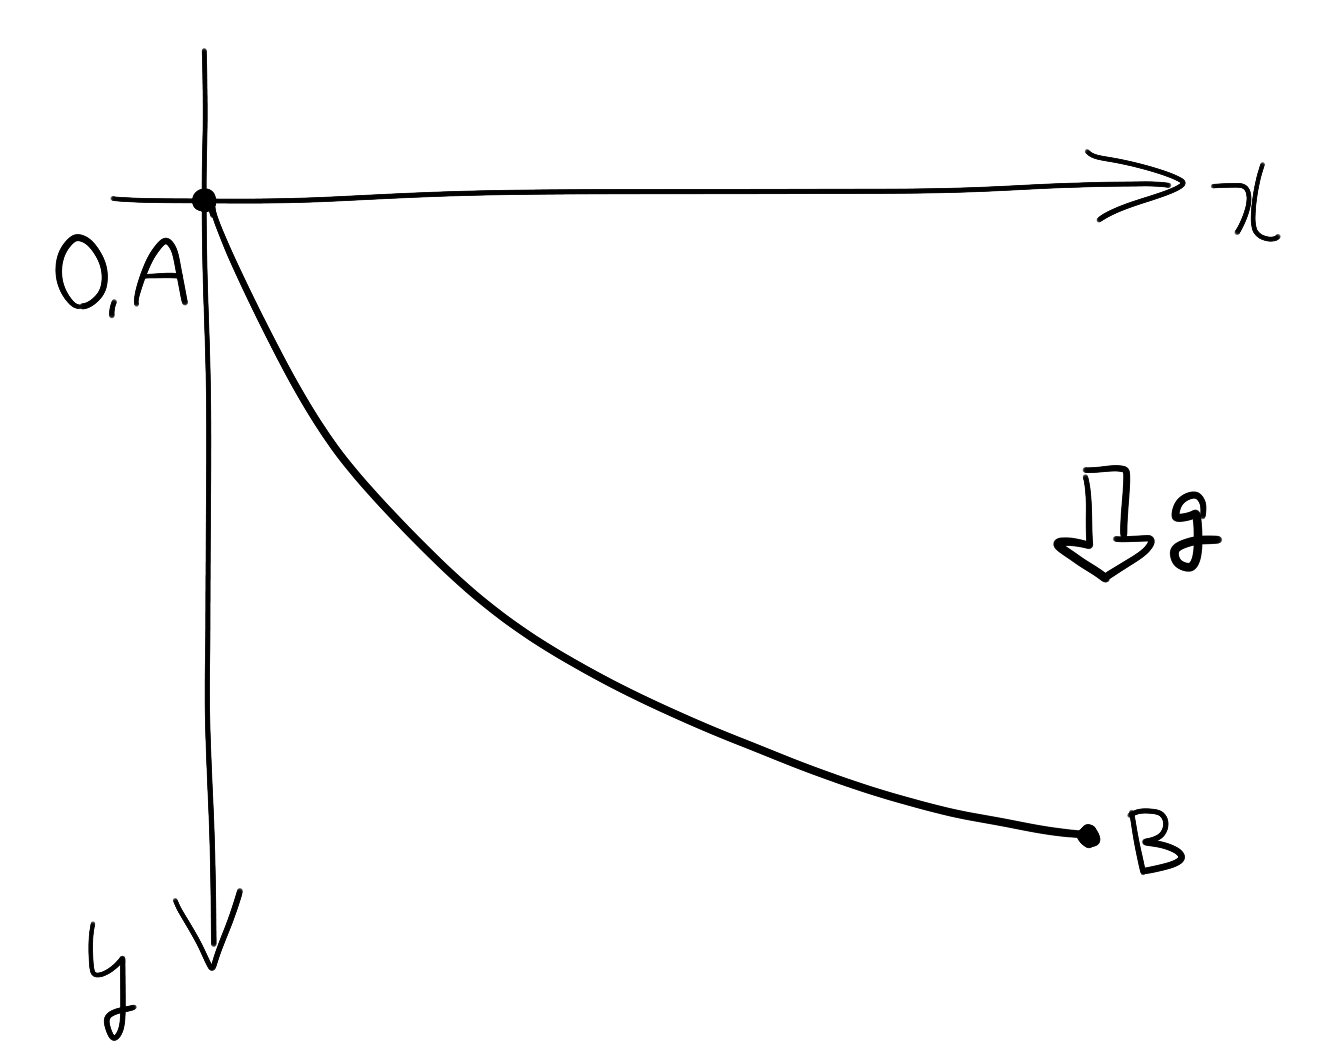
\includegraphics[width = 5cm]{nakayama1/image/zahyou}
\end{wrapfigure}
この曲線の式を求めるために、まずは坂道の地点Aから地点Bまでボールが転がるのにかかる時間を式で表そう。まずは図のように座標をとる。地点Aを原点Oとする。また、$y$軸を下向きにとっているので注意。


ボールの微小変位$\dd L$は三平方の定理より
\begin{align*}
  \dd L = \sqrt{\dd x^2 + \dd y^2}
        = \sqrt{1 + \left( \frac{\dd y}{\dd x} \right)^2} \,\,\dd x
\end{align*}\par
ボールの速度を$v$、重力加速度を$g$とすれば、力学的エネルギー保存則より
\begin{align*}
  v = \sqrt{2gy}
\end{align*}
であるから、ボールが$\dd L$だけ転がるのにかかる微小時間$\dd t$は
\begin{align*}
  \dd t = \frac{\dd L}{v} = \sqrt{\frac{1 + (y')^2}{2gy}} \,\,\dd x
\end{align*}\par
よって求める時間はこれを積分して
\begin{align*}
  T = \int_A^B \dd t = \int_A^B \sqrt{\frac{1 + (y')^2}{2gy}} \,\,\dd x
\end{align*}
と表すことができる。\par
今知りたいのはこの$T$を最小にするような$y$の形である。しかし、それを考えるには変分法という新しい技を身につけなければならない。\par
次節では変分法について簡単に解説し、必要な公式を導出する。

\subsection{変分法}

\subsubsection{変分法とは}
微分を勉強した時に、$y = f(x)$が最小値をとるときの$x$の値を求める問題を考えたことがあると思う。もし端点以外に$y$が最小値をとるときがあるとすれば、$y$はそこで極値をとる。つまり$y$の導関数$y'$が$y' = 0$となるときの$x$を調べれば$y$が最小値をとる可能性のある$x$を見つけることができる(極大値をとるかもしれないが)。\par
今回の問題もこの方法で解決できそうだが、少し勝手が違う。先ほど求めた$T$は積分された形にはなっているが、$y$の関数となっている。しかしその$y$は$x$の関数となっている。つまり$T$は関数の関数という形になっている。今回の$T$のように、関数を変数にとるような関数は汎関数と呼ばれている。\par
微分法が関数について研究するところであるとすると、変分法は汎関数について研究するところであると言える。

\subsubsection{汎関数$F(y)$の極値}

ここでは$T$を少し一般化した
$$ F(y) := \int_a^b f(x,y(x),y'(x)) \,\dd x$$
で定義された$F(y)$について考える。知りたいのはこの$F(y)$が極値をとるときの$y$の形である。\par
そこで以下のように、$y$の形を少し変えたものとして$y_\epsilon$を定義する。
$$ y_\epsilon (x) := y(x) + \epsilon h(x) $$
ただし、$h(x)$は$h(a) = h(b) = 0$を満たす任意の関数\footnote{端点は固定するという意味。坂道の話でいうとスタート地点とゴール地点は変えないということ。}、$\epsilon$は任意の実数であるとする。このように定義された$y_\epsilon$を$y$の$h$方向の変分という。\par
そうすると、$y_\epsilon$は$\epsilon$の関数であるから、$F(y_\epsilon)$も$\epsilon$の関数となる。\par
\begin{figure}[H]
  \centering
  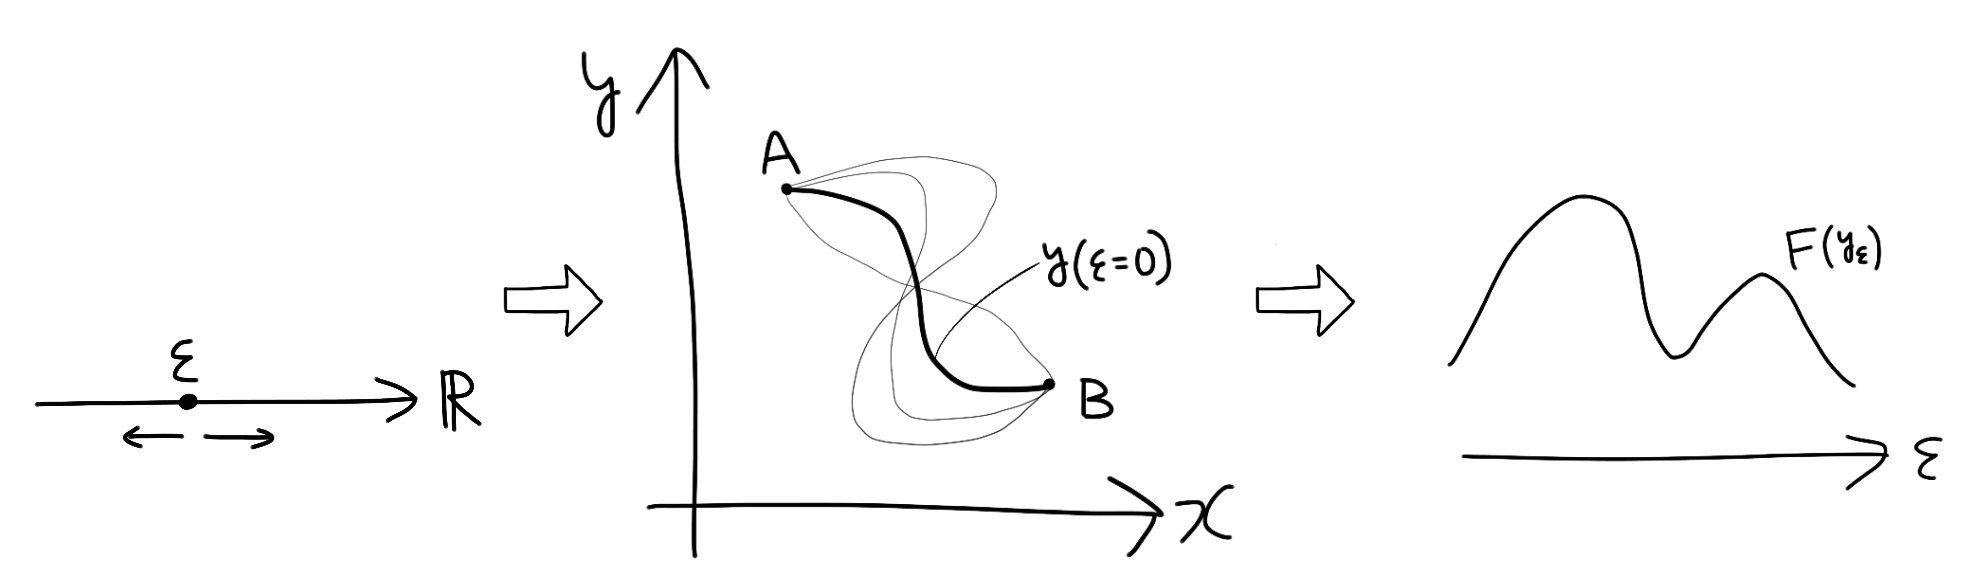
\includegraphics[width = 100mm]{nakayama1/image/henbun.png}\\
  {\small 変分原理のイメージ図}
\end{figure}

$F(y_\epsilon)$が$\epsilon$の関数ならば、$F(y_\epsilon)$は$\epsilon$で微分可能である。つまり微分法のときと同じように考えて$\dfrac{\dd F(y_\epsilon)}{\dd \epsilon} = 0$のとき$F(y_\epsilon)$は極値をとることがわかる。
よって$\dfrac{\dd F(y_\epsilon)}{\dd \epsilon} = 0$とおけば、$F(y_\epsilon)$が極値をとるときの$\epsilon$の値がわかる。$\epsilon$の値がわかれば、それから$y_\epsilon$がわかる。つまりその$y_\epsilon$に対して$F(y_\epsilon)$は極値をとる。
以上のことから、もし$y_\epsilon = y$($\epsilon = 0$のとき)で$F(y_\epsilon)$が極値をとるなら
$$\left. \dfrac{\dd}{\dd \epsilon}F(y_\epsilon) \right|_{\epsilon = 0} = 0$$
が成り立つ。つまりこれを満たす$y_\epsilon$($=y$)が$F$が極値をとるときの関数となっている。また
$$\delta F := \left. \dfrac{\dd}{\dd \epsilon}F(y_\epsilon) \right|_{\epsilon = 0}$$
で定義される$\delta F$を汎関数$F$の第一変分といい、$\delta F = 0$を満たす点$y$を$F$の臨界点または停留点という。\par
以上が変分法についての簡単な(?)説明である。最後に微分法と変分法の対応を書いておく。

\begin{table}[H]
  \begin{center}
    {\gt \small 微分法と変分法の対応}\\
    \begin{tabular}{cc}
      微分 & 変分\\ \hline
      関数$f$ & 汎関数$F$\\
      関数$f$の微分$f'=0$ & 汎関数$F$の変分$\delta F=0$\\
      関数$f$が極値をとる点$x$ & 汎関数$F$の臨界点$y$
    \end{tabular}
  \end{center}
\end{table}

\subsubsection{オイラー=ラグランジュの方程式}

前節では$F(y_\epsilon)$が極値となるような$y_\epsilon$が知りたければ、汎関数$F$の第一変分$\delta F = 0$を満たす$y_\epsilon$を見つければよいということがわかった。この節では$\delta F = 0$を計算して、オイラー=ラグランジュの方程式を導く。\par
まずは$F(y)$の定義を思い出す。
$$ F(y) = \int_a^b f(x,y(x),y'(x)) \,\dd x$$
よって$F$の第一変分は
\begin{align*}
  \delta F
  = \left. \dfrac{\dd}{\dd \epsilon}F(y_\epsilon) \right|_{\epsilon = 0}
  &= \left. \frac{\dd}{\dd \epsilon} \int_a^b f(x,y_\epsilon (x),y'_\epsilon (x)) \,\dd x \right|_{\epsilon = 0} \\
  &= \left. \int_a^b \frac{\dd f}{\dd \epsilon} \,\dd x \right|_{\epsilon = 0}
\end{align*}
合成関数の微分法より
\begin{align*}
  \hspace{43mm} &= \left. \int_a^b \left( \frac{\partial f}{\partial y_\epsilon} \cdot \frac{\dd y_\epsilon}{\dd \epsilon} + \frac{\partial f}{\partial y_\epsilon'} \cdot \frac{\dd y_\epsilon'}{\dd \epsilon} \right) \dd x \right|_{\epsilon = 0} \\
  &= \left. \int_a^b \left( \frac{\partial f}{\partial y_\epsilon} \cdot \frac{\dd y_\epsilon}{\dd \epsilon} + \frac{\partial f}{\partial y_\epsilon'} \cdot \frac{\dd}{\dd x} \frac{\dd y_\epsilon}{\dd \epsilon} \right)\dd x \right|_{\epsilon = 0} \\
  &= \left. \int_a^b \left( \frac{\partial f}{\partial y_\epsilon} \cdot h(x) + \uwave{\frac{\partial f}{\partial y_\epsilon'} \cdot \frac{\dd}{\dd x}h(x)} \right)\dd x \right|_{\epsilon = 0}
\end{align*}
ここで\uwave{第2項}を部分積分すると
\begin{align*}
  \int_a^b \frac{\partial f}{\partial y_\epsilon'} \cdot \frac{\dd}{\dd x}h(x) \,\dd x
  &= \left[ \frac{\partial f}{\partial y_\epsilon'} \cdot h(x) \right]_a^b - \int_a^b \frac{\dd}{\dd x}\frac{\partial f}{\partial y_\epsilon'} \cdot h(x) \,\dd x
\end{align*}
$h(a) = h(b) = 0$より
$$\left[ \frac{\partial f}{\partial y_\epsilon'} \cdot h(x) \right]_a^b = 0$$
となるので
\begin{align*}
  \int_a^b \frac{\partial f}{\partial y_\epsilon'} \cdot \frac{\dd}{\dd x}h(x) \,\dd x
  &= - \int_a^b \frac{\dd}{\dd x}\frac{\partial f}{\partial y_\epsilon'} \cdot h(x) \,\dd x
\end{align*}
元の式に戻して
\begin{align*}
  \delta F &= \left. \int_a^b \left( \frac{\partial f}{\partial y_\epsilon} - \frac{\dd}{\dd x}\frac{\partial f}{\partial y_\epsilon'} \right)h(x) \,\dd x \right|_{\epsilon = 0} \\
  &= \int_a^b \left( \frac{\partial f}{\partial y} - \frac{\dd}{\dd x}\frac{\partial f}{\partial y'} \right)h(x) \,\dd x
\end{align*}
よって$F$が極値をもつ条件は
\begin{align*}
  \int_a^b \left( \frac{\partial f}{\partial y} - \frac{\dd}{\dd x}\frac{\partial f}{\partial y'} \right)h(x) \,\dd x = 0
\end{align*}
が成り立つことである。$h(x)$は任意関数であるから、これが常に成り立つとすると
\begin{align*}
  \frac{\partial f}{\partial y} - \frac{\dd}{\dd x}\frac{\partial f}{\partial y'} = 0
\end{align*}
という方程式が得られる。これをオイラー=ラグランジュの方程式と呼ぶ。\par
あとはこの方程式に$f = T = \sqrt{\dfrac{1 + (y')^2}{2gy}}$を代入して解けばいいのだが、計算が大変になるので、もう少しこの方程式を変形しよう。

\subsubsection{ベルトラミの公式}
前節でオイラー=ラグランジュの方程式を導出したときは$f = f(x,y,y')$としていたが、今回考えたい$T$は$x$を陽に(直接には)含んでいないので、オイラー=ラグランジュの方程式はもう少し簡単な形に変形することができる。$f = f(y,y')$としてもう少し考えよう。\par
$f$の全微分は
$$\dd f(y,y') = \frac{\partial f}{\partial y}\dd y + \frac{\partial f}{\partial y'}\dd y'$$
であるから、両辺$\dd x$で割って
\begin{align*}
  \frac{\dd f}{\dd x} &= \frac{\partial f}{\partial y} \frac{\dd y}{\dd x} + \frac{\partial f}{\partial y'} \frac{\dd y'}{\dd x} \\
  &= \uwave{y'\frac{\partial f}{\partial y}} + \frac{\dd y'}{\dd x} \frac{\partial f}{\partial y'}
\end{align*}\par
一方、オイラー=ラグランジュの方程式の両辺に$y'$をかけると
$$0 = y'\left( \frac{\partial f}{\partial y} - \frac{\dd}{\dd x}\frac{\partial f}{\partial y'} \right)
= \uwave{y'\frac{\partial f}{\partial y}} - y'\frac{\dd}{\dd x}\frac{\partial f}{\partial y'}$$\par
この2式から$\uwave{y'\dfrac{\partial f}{\partial y}}$を消去すると
\begin{align*}
  \frac{\dd f}{\dd x} &= \frac{\dd y'}{\dd x} \frac{\partial f}{\partial y'} + y'\frac{\dd}{\dd x}\frac{\partial f}{\partial y'} \\
  &= \frac{\dd}{\dd x} \left( y'\frac{\partial f}{\partial y'} \right)
\end{align*}\par
両辺$x$で積分して
\begin{align*}
  \int \frac{\dd f}{\dd x} \,\dd x &= \int \frac{\dd}{\dd x} \left( y'\frac{\partial f}{\partial y'} \right) \dd x \\
  f &= y'\frac{\partial f}{\partial y'} + C
\end{align*}\par
よって
\begin{align*}
  \qquad\qquad f - y'\frac{\partial f}{\partial y'} = C \qquad\quad\text{($C$は任意定数)}
\end{align*}\par
という方程式が得られる。これをベルトラミの公式と呼ぶ。

\subsection{最速降下曲線の形}
変分法の話が長くなったが、あとはベルトラミの公式から$T$が極値をとるときの$y$(これが知りたかったもの)がわかるので、$f = T$を代入して計算してみよう。
\begin{align*}
  C &= T - y'\frac{\partial T}{\partial y'} \\
  &= \sqrt{\frac{1 + (y')^2}{2gy}} - y'\frac{\partial}{\partial y'} \sqrt{\frac{1 + (y')^2}{2gy}} \\
  &= \sqrt{\frac{1 + (y')^2}{2gy}} - \frac{y'}{\sqrt{2gy}} \frac{\partial}{\partial y'} \sqrt{1 + (y')^2} \\
  &= \sqrt{\frac{1 + (y')^2}{2gy}} - \frac{y'}{\sqrt{2gy}} \frac{y'}{\sqrt{1 + (y')^2}} \\
  &= \frac{1 + (y')^2 - (y')^2}{\sqrt{2gy\{1 + (y')^2\}}} \\
  &= \frac{1}{\sqrt{2gy\{1 + (y')^2\}}}
\end{align*}\par
よって
$$\sqrt{2gy\{1 + (y')^2\}} = \frac{1}{C}$$\par
両辺2乗して
\begin{align*}
  2gy\{1 + (y')^2\} &= \frac{1}{C^2} \\
  y\{1 + (y')^2\} &= \frac{1}{2gC^2}
\end{align*}\par
定数を$2r \equiv \frac{1}{2gC^2}$と置き直して
\begin{align*}
  y\{1 + (y')^2\} &= 2r \\
  (y')^2 &= \frac{2r}{y} - 1
\end{align*}
ここで両辺ルートをとるが、坂道なので$y' > 0$のときだけ考える。
\begin{align*}
  \frac{\dd y}{\dd x} \equiv y' &= \sqrt{\frac{2r}{y} - 1} \\
  &= \frac{\sqrt{2ry - y^2}}{y} \\
  &= \frac{\sqrt{r^2 - (r^2 - 2ry + y^2)}}{y} \\
  &= \frac{ \sqrt{r^2 - (r - y)^2} }{y}
\end{align*}
よって
\begin{align*}
  \dd x & = \frac{y}{ \sqrt{r^2 - (r - y)^2} }\,\dd y
\end{align*}
両辺積分すると
\begin{align*}
  x = \int \frac{y}{ \sqrt{r^2 - (r - y)^2} }\,\dd y
\end{align*}
$y = r(1 - \cos\theta)$とおくと、$\dd y = r\sin\theta \,\dd \theta$であるから
\begin{align*}
  x &= \int \frac{r(1 - \cos\theta)}{r \sqrt{1 - \cos^2 \theta}}\,r\sin\theta\,\dd \theta \\
  &= \int r(1 - \cos\theta)\,\dd \theta \\
  &= r(\theta - \sin\theta) + \mathrm{const.}
\end{align*}
原点を通るとして、$x = 0$のとき$y = 0$。またこのとき$\theta = 0$であるから$\mathrm{const.} = 0$。よって
\begin{align*}
  \begin{cases}
    \, x = r(\theta - \sin\theta)\\
    \, y = r(1 - \cos\theta)
  \end{cases}
\end{align*}
と媒介変数表示できた。これはサイクロイドである。

\begin{figure}[H]
  \centering
  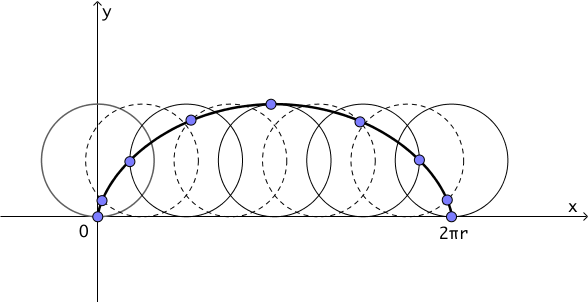
\includegraphics[width=8cm]{nakayama1/image/cyco}\\
  {\small サイクロイドの図。円を転がすとき、円周に固定した点が描く軌道がサイクロイド。\\
  今回の話では$y$軸を下向きを正としていたことに注意。つまりこれを上下反転したものになる。}
\end{figure}

%
\clearpage
\section*{参考文献}
\begin{enumerate}
  \item[] \hspace{-20pt}{\gt インボリュート曲線}
  \item インボリュート曲線 - Wikipedia,「\url{https://ja.wikipedia.org/wiki/インボリュート曲線}」
  \item 伸開線 - Wikipedia,「\url{https://ja.wikipedia.org/wiki/伸開線}」
  \item[] \hspace{-20pt}{\gt トラクトリックス}
  \item トラクトリックス - Wikipedia, 「\url{https://ja.wikipedia.org/wiki/トラクトリックス}」
  \item Tractrix.pdf,「\url{http://izumi-math.jp/M_Matumoto/Tractrix.pdf}」
  \item[] \hspace{-20pt}{\gt 変分法}
  \item 変分法 - Wikipwdia,「\url{https://ja.wikipedia.org/wiki/変分法}」
  \item 変分法1 [物理のかぎしっぽ], 「\texttt{http://hooktail.sub.jp/mathInPhys/variations1/}」
  \item @minami106, 変分法の入門編, 「\texttt{http://minami106.web.fc2.com/math/henbun2.pdf}」
    \item 西山豊, 最速降下問題,
    「\url{http://www.osaka-ue.ac.jp/zemi/nishiyama/math2010j/cycloid_j.pdf}」
  \item 山上滋, 微積分II,\\
  「\url{https://www.math.nagoya-u.ac.jp/~yamagami/teaching/calculus/cal2011akib.pdf}」
\end{enumerate}





%
 \clearpage
% タイトル
\chapter{角の三等分問題}
\vspace{-45pt} %高さ調整
\begin{flushright}
  {\bf \large 理工学部 物理科学科 2回生} \\ \vspace{3pt} %所属
  {\bf \large 中山 敦貴} \\ \vspace{30pt} %名前
\end{flushright}

% 序論
\section*{はじめに}
高2のころから読み始めた結城浩さん著の「数学ガール」であるが、今年の夏休みにようやく第5巻であるガロア理論を読み終えることができた。よって今回の内容はガロア理論である。と言いたいところだが、ガロア理論なんて簡単に理解できるものじゃないし、代数学のラスボスである(適当)。ということで今回は代数学超入門として、作図可能数の話をすることにする。また、他にも2冊ガロア理論超入門書を読んで、方程式の面白い話があったのでそれも紹介したかったが、今回の会誌には入れることができなかった。今後作るかもしれないバージョンアップ版に期待してほしい。

%
\section{角の三等分問題とは}
有名な作図問題のひとつに、角の三等分問題というものがある。今回はこれ考えるわけであるが、まずは数学的にどのような問いになっているか考えよう。
\begin{itembox}[l]{\bf 角の三等分問題(?)}
{\bf 問い} 与えられた角を三等分できるか?\\
{\bf 解答} 分度器使えばできる。
\end{itembox}
\par 問いたいことはそういうことじゃない。もう少しちゃんと問いを立てよう。\\

\begin{itembox}[l]{\bf 角の三等分問題}
{\gt 定規}と{\gt コンパス}だけを使って、与えられた{\gt 任意の}角を三等分できるか?
\end{itembox}

\begin{quote}
{\gt 定規}  :与えられた2点を通る直線が引ける。\\
{\gt コンバス}:与えられた2点の片方を中心とし、他方を通る円が描ける。
\end{quote}

\begin{itemize}
\item[{\gt (注)}]
\item 初めに2点は与えられているとする。
\item 定規とコンパスは繰り返し使える(ただし有限回とする)。
\item ある時点で使える点は、そこまでに作図した「直線と円」「直線と直線」「円と円」の交点だけとする。
\item コンパスで円を書いた後、コンパスの針を他の点に移して円を描いてもよいとする(=同じ半径の円を別の点の周りに描いてもよい)。
\end{itemize}

つまり、三等分できないような角が1つでもあれば、”定規とコンパスだけでは、与えられた任意の角を三等分{\gt できない}”というのがこの角三等分問題への解答となる。オチを言ってしまうと、実際そうなっている。つまり定規とコンパスだけで三等分できないような角が存在する。それも身近なところに。

%
\section{作図可能数}

\subsection{作図可能数とは}
作図には{\gt 点}が必要だから、{\gt 作図可能な点}$(x,y)$を考えることになる。作図可能点の座標成分$x,y$を{\gt 作図可能数}と呼ぶ。\par
では、いったいどんな数が作図可能数になっているだろうか?\par
まず初めに、原点$(0,0)$と$(1,0)$の2点が与えられているとする。
原点$(0,0)$と$(1,0)$を通る直線を引けば$x$軸ができる。さらにコンパスを使って、$x$軸上に整数の点を作図できる。$x$軸に対して原点を通るように垂線を引けば$y$軸もでき、$y$軸上にも整数の点が作図できる。つまり格子点が作図できることになる。よって、{\gt 整数は作図可能数}となる。

\newpage
\subsection{四則演算と開平}
以下のようにすれば、定規とコンパスで加減乗除ができる。
\begin{figure}[H]
  \begin{center}
    \begin{tabular}{c}
        \begin{minipage}{0.5\hsize}
          \begin{center}
            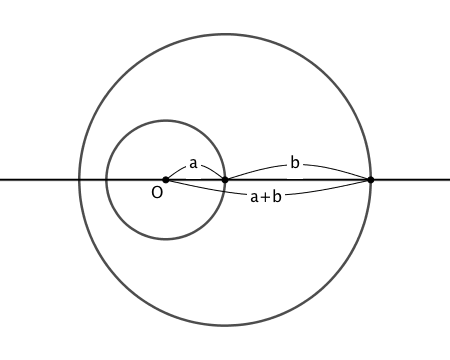
\includegraphics[clip, width=5.5cm]{nakayama2/image/a+b.png}
            \hspace{1.6cm} \bf $a$と$b$から$a+b$をつくるの図
          \end{center}
        \end{minipage}

        \begin{minipage}{0.5\hsize}
          \begin{center}
            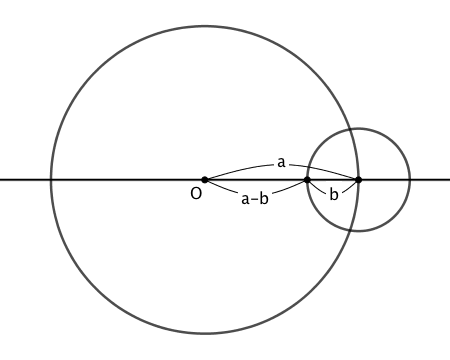
\includegraphics[clip, width=5.5cm]{nakayama2/image/a-b.png}
            \hspace{1.6cm} \bf $a$と$b$から$a-b$をつくるの図
          \end{center}
        \end{minipage}
    \end{tabular}
  \end{center}
\end{figure}\par

\begin{figure}[H]
  \begin{center}
    \begin{tabular}{c}
        \begin{minipage}{0.5\hsize}
          \begin{center}
            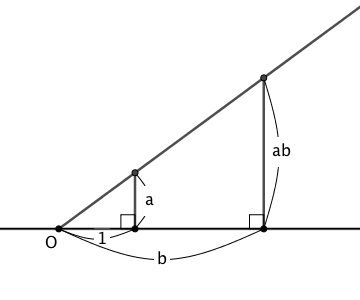
\includegraphics[clip, width=5.5cm]{nakayama2/image/ab.png}
            \hspace{1.6cm} \bf $a$と$b$から$ab$をつくるの図
          \end{center}
        \end{minipage}

        \begin{minipage}{0.5\hsize}
          \begin{center}
            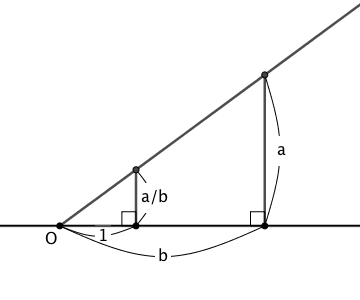
\includegraphics[clip, width=5.5cm]{nakayama2/image/a_b.png}
            \hspace{1.6cm} \bf $a$と$b$から$\frac{a}{b}$をつくるの図
          \end{center}
        \end{minipage}
    \end{tabular}
  \end{center}
\end{figure}\par\par\par

整数が作図可能で加減乗除ができるので、整数の加減乗除で作られる{\gt 有理数は作図可能数}となる。
作図で加減乗除ができるので、作図可能数は{\gt 体}$(\DD とする)$である。
$$\mathbb{Z} \subset \mathbb{Q} \subset \DD \subset \mathbb{R}$$
さらに、定規とコンパスで開平もできる。下図で、三平方の定理より、$\mathrm{BP} = \sqrt{a}$となっていることがわかる。

\begin{figure}[H]
  \centering
  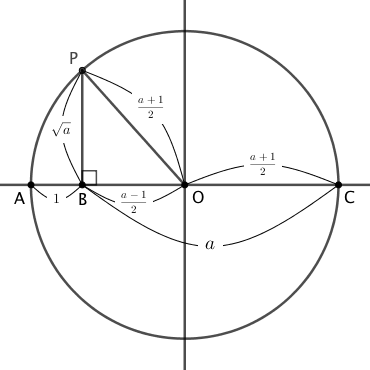
\includegraphics[clip, width=7cm]{nakayama2/image/root.png}\\
  \bf $a$から$\sqrt{a}$をつくるの図
\end{figure}

よって
\begin{align*}
  \sqrt{a} \in \DD \qquad (a \in \mathbb{Q},\, a > 0)
\end{align*}
さらに開平を繰り返してもよい
\begin{align*}
  a \in \DD \Rightarrow \sqrt{a} \in \DD \qquad (a > 0)
\end{align*}
つまり、$a$を正の有理数として次のようなことがいえる:
\begin{align*}
  \sqrt{a} \in \DD\\
  \sqrt{\sqrt{a}} \in \DD\\
  \sqrt{\sqrt{\sqrt{a}}} \in \DD\\
\end{align*}
さらにそうして作った数の加減乗除もできるので、$p,q,r$を正の有理数として次のようなこともいえる:
\begin{align*}
  \sqrt{\sqrt{p} + \sqrt{q}} \in \DD\\
  \sqrt{\sqrt{p} + \sqrt{\sqrt{q}}} + \sqrt{r} \in \DD\\
  \sqrt{\sqrt{\sqrt{p} + \sqrt{\sqrt{q}}} + \sqrt{r}} \in \DD\\
\end{align*}\par
整数から始めて加減乗除と開平を繰り返し使えばどんな数でも作れそうだが、そんなことはない。例えば$\sqrt[3]{2}$は整数の加減乗除と開平だけからは作れない。
\begin{quote}
  じゃあ結局どんな数が作図できるの?
\end{quote}
直線は1次方程式、円は2次方程式で書ける。その交点(作図可能点)は連立方程式で求められる。連立方程式には1次方程式と2次方程式しか出てこないので、作図可能数は1次方程式か2次方程式の解になるものしかない。
よって作図可能数は
\begin{quote}
  《加減乗除と開平の繰り返しで作れる数》
\end{quote}
であることがわかる。

%
\section{本題}
\subsection{$20^\circ$の作図}
それでは、作図可能数を用いて角の三等分問題を考える。\par
$20^\circ$が作図可能かどうか調べよう。もし$20^\circ$が作図可能でなければ、それが角三等分問題への解答となる。
$$
20^\circ\text{が作図可能} \,\,\Longleftrightarrow\,\, \cos 20^\circ \text{が作図可能数}
$$
であるから$\cos 20^\circ$が作図可能数か考えればよい。
\begin{figure}[H]
  \centering
  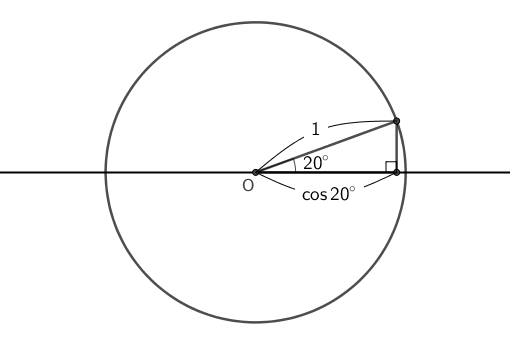
\includegraphics[clip, width=5.5cm]{nakayama2/image/cos20do.png}\\
  \small $20^\circ$が作図できれば$\cos 20^\circ$も作図可能。逆も言える。
\end{figure}

コサインの三倍角公式「$\cos 3\theta = 4\cos^3 \theta - 3\cos\theta$」で$\theta = 20^\circ$としてみると
\begin{align*}
  \cos 60^\circ = 4\cos^3 20^\circ - 3\cos 20^\circ \\
  \frac{1}{2} = 4\cos^3 20^\circ - 3\cos 20^\circ \\
  8\cos^3 20^\circ - 6\cos 20^\circ - 1 = 0
\end{align*}
$x = 2\cos 20^\circ$とおくと
$$ x^3 - 3x -1 = 0 $$
となり、この3次方程式の解の1つが$2\cos 20^\circ$になっている。
よって、もしこの3次方程式が作図可能数を1つも解に持たないならば、$2\cos 20^\circ$つまり$\cos 20^\circ$は作図可能数でないことになる。
したがって$20^\circ$は作図不可能となり、三等分できない角として$60^\circ$が与えられる。


\subsection{証明!証明!証明!}
\subsubsection{証明の概要}
もうただ真面目に証明してしまうことにする。
\begin{itembox}[l]{\bf 定義}
  $0$以上の整数$n$について、体$\KK_n$を以下のように定義する:
  \begin{align*}
    \begin{cases}
    \,\KK_0 &= \mathbb{Q}\\
    \,\KK_{k+1} &= \{p + q\sqrt{r} \,\,|\,\, p,q,r \in \KK_k, \sqrt{r} \notin \KK_k\}\\
    & \qquad\text{\footnotesize (ただし$k = 0,1,2,...$で$r$は$k$ごとに固定する)}\\
    &= \KK_k (\sqrt{r}) \qquad\text{$r \in \KK_k, \sqrt{r} \notin \KK_k$}
    \end{cases}
  \end{align*}
\end{itembox}
\,
\begin{itembox}[l]{\bf 定義}
  命題$P(n)$:方程式$x^3 -3x -1 = 0$は、体$\KK_n$に解を持たない
\end{itembox}
\,
\begin{itembox}[l]{\bf 証明すべきこと}
  以下のステップ(a)とステップ(b)を示せば、数学的帰納法により、どんな$0$以上の整数$n$についても$P(n)$が成り立つ。すなわち、方程式$x^3 -3x -1 = 0$は、体$\KK_n$に解を持たない。
  \begin{quote}
    ステップ(a):$P(0)$\\
    ステップ(b):$P(k) \Rightarrow P(k+1)$
  \end{quote}
\end{itembox}

% \clearpage
\subsubsection{ステップ(a)}
\begin{itembox}[l]{\bf ステップ(a)}
  方程式$x^3 -3x -1 = 0$は有理数体$\mathbb{Q}$に解を持たない
\end{itembox}
{\bf (証明)}\par
方程式$x^3 -3x -1 = 0$は有理数体$\mathbb{Q}$に解を持つと仮定する。\par
すると解$x$は整数$A,B$を用いて次のように表せる:
$$ x = \frac{A}{B} \qquad (B \neq 0,\, AとBは互いに素)$$\par
これを$x^3 -3x -1 = 0$に代入して整理すると
$$ A^3 = (3A + B)B^2 $$\par
ここで$A$の素因数に注目する。まず$A \neq 0,1,-1$であることは、それぞれ代入してみればわかる。また、$A < 0$のときは$B$の符号を反転させればよいので、$A > 0$の場合だけ考える。\par
$A$の素因数を$p$とすると、左辺$A^3$は$p$で割り切れる。しかし右辺の$(3A+B)$も$B^2$も$p$で割り切れない。$\rightarrow$矛盾
\begin{flushright}
  (証明終)
\end{flushright}

\subsubsection{ステップ(b)}

あとで使うので、まず補題を1つ証明しておく。$\KK = \mathbb{Q}$のときはもう中学生か高校生のころに証明したことがあると思う。それの一般化である。
\begin{itembox}[l]{\bf 補題}
$\KK$を体とし、$p,q,r \in \KK, \sqrt{r} \notin \KK$のとき
$$ p + q\sqrt{r} = 0 \,\,\Longleftrightarrow\,\, p = q = 0$$
\end{itembox}
{\bf (証明)}\\
$(\Leftarrow)$であること \par $p = q = 0$なら明らかに$p + q\sqrt{r} = 0$ \\
$(\Rightarrow)$であること \par
仮定より$p + q\sqrt{r} = 0$。 \par
$q = 0$ならば$p = 0$。\par
$q \neq 0$のとき、$\sqrt{r} = -\frac{p}{q}$。\par
ここで$\sqrt{r} \notin \KK$ であるが、$-\frac{p}{q} \in \KK$となっている。 $\rightarrow$矛盾\par
よって$q = 0$。
\begin{flushright}
  (証明終)
\end{flushright}


\begin{itembox}[l]{\bf ステップ(b)}
方程式$x^3 -3x -1 = 0$は体$\KK$に解を持たない $\Longrightarrow$ 体$\KK(\sqrt{r})$にも解を持たない
\end{itembox}
{\bf (証明)}\par
前提条件:方程式$x^3 -3x -1 = 0$は体$\KK$に解を持たない\par
仮定:方程式$x^3 -3x -1 = 0$は体$\KK(\sqrt{r})$に解を持つ\par
その解を$x = p + q\sqrt{r} \in \KK(\sqrt{r})$とする。$(p,q,r \in \KK, \sqrt{r} \notin \KK)$\par
ここで$q \neq 0, r \neq 0$である。(\,$\because$ 前提条件に反する)\par
$x^3 -3x -1 = 0$に$x = p + q\sqrt{r}$を代入して整理すると
$$ (p^3 - 3p - 1 + 3pq^2r) + (3p^2 + q^2r - 3)q\sqrt{r} = 0 $$
となる。ここで$P = (p^3 - 3p - 1 + 3pq^2r), Q = (3p^2 + q^2r - 3)q$とおけば、$P,Q \in \KK$であり、
$$ P + Q\sqrt{r} = 0 $$
と書ける。\par
また、$x^3 -3x -1$に$x = p - q\sqrt{r}$を代入してみると
\begin{align*}
  x^3 -3x -1 &= (p^3 - 3p - 1 + 3pq^2r) - (3p^2 + q^2r - 3)q\sqrt{r}\\
  &= P - Q\sqrt{r}
\end{align*}
となる。\par
ここで補題より$P = Q = 0$であり、$P - Q\sqrt{r} = 0$となる。すなわち$p + q\sqrt{r}$が解のとき、$p - q\sqrt{r}$も解となっている。\par
3次方程式は3つの解を持つが、そのうちの2つは既に分かっている。
\begin{align*}
  \begin{cases}
    \,\alpha &= p + q\sqrt{r}\\
    \,\beta &= p - q\sqrt{r}\\
    \,\gamma &= \,\,\,?
  \end{cases}
\end{align*}\par
3つ目の解$\gamma$は解と係数の関係$\alpha + \beta + \gamma = 0$より
\begin{align*}
  \gamma &= - \alpha - \beta \\
  &= -(p + q\sqrt{r}) - (p - q\sqrt{r})\\
  &= -2p
\end{align*}\par
ここで$p \in \KK$より$\gamma = -2p \in \KK$となるが、これは前提条件に反する。\par
よって仮定が否定され、
\begin{quote}
  《方程式$x^3 -3x -1 = 0$は体$\KK$に解を持たない》という前提条件で\\
  《方程式$x^3 -3x -1 = 0$は体$\KK(\sqrt{r})$に解を持たない》
\end{quote}
ということが証明できた。
\begin{flushright}
  (証明終)
\end{flushright}

\subsection{拡大次数を用いた別の証明}
体の話をいろいろと知っているともっとスマートに証明ができる。これからその証明を紹介するが、僕も体の話はよく知らない。なのでいくつかの定理というか拡大次数を求めるための公式を証明はせずに、具体例をいくつか見てもらうことでその定理が正しいと納得してもらうことにする。
\begin{itembox}[l]{\bf 拡大体$\mathbb{Q}(a)/\mathbb{Q}$}
$\mathbb{Q}$:有理数体\par
$\mathbb{Q}(a)$:有理数体$\mathbb{Q}$に数$a$を添加した体\par
としたとき、
$\mathbb{Q}(a)$は$\mathbb{Q}$の{\gt 拡大体}であることを$\mathbb{Q}(a)/\mathbb{Q}$と書く。
\end{itembox}

\begin{itembox}[l]{\bf $\mathbb{Q}(a)/\mathbb{Q}$の拡大次数}
$\mathbb{Q}(a)$を$\mathbb{Q}$上の線形空間とみなしたときの{\gt 次元}(基底の要素数)を$\mathbb{Q}(a)/\mathbb{Q}$の{\gt 拡大次数}といい、$[\mathbb{Q}(a):\mathbb{Q}]$と書く。\\
拡大次数が$n$になる体の拡大を{\gt $n$次拡大}という。
\end{itembox}
{\gt 例}\par
$\mathbb{Q}(\sqrt{2}) = \{p + q\sqrt{2} \,\,|\,\, p,q \in \mathbb{Q}\}$ \par
$\mathbb{Q}(\sqrt{2})$に属する任意の数は$\{ 1, \sqrt{2} \}$という2つの基底を使って$p + q\sqrt{2}$と書ける。\par
よって、$\mathbb{Q}(\sqrt{2})/\mathbb{Q}$の拡大次数は
$$[\mathbb{Q}(a):\mathbb{Q}] = 2$$
となり、この拡大は2次拡大である。

\begin{itembox}[l]{\bf 拡大次数の積の定理}
$\mathbb{Q}$に数$a,b$を添加した拡大体
$$\mathbb{Q}(a,b) = \mathbb{Q}(a)(b) \quad \text{($\mathbb{Q}(a)$に$b$を添加した体)}$$
の拡大次数は
\begin{align*}
  [\mathbb{Q}(a,b):\mathbb{Q}] &= [\mathbb{Q}(a)(b):\mathbb{Q}]\\
  &= [\mathbb{Q}(a):\mathbb{Q}] \times [\mathbb{Q}(a)(b):\mathbb{Q}(a)]
\end{align*}
で計算できる。
\end{itembox}
{\gt 例1}
\begin{align*}
  [\mathbb{Q}(\sqrt{2},\sqrt{3}):\mathbb{Q}] &= [\mathbb{Q}(\sqrt{2})(\sqrt{3}):\mathbb{Q}]\\
  &= [\mathbb{Q}(\sqrt{2}):\mathbb{Q}] \times [\mathbb{Q}(\sqrt{2})(\sqrt{3}):\mathbb{Q}(\sqrt{2})]\\
  &= 2 \times 2 = 4
\end{align*}\par
実際、基底は$\{ 1,\sqrt{2},\sqrt{3},\sqrt{6} \}$の4つ。\\\\
{\gt 例2}
\begin{align*}
  [\mathbb{Q}(\sqrt{2},\sqrt{3},\sqrt{5},\sqrt{7}):\mathbb{Q}] &= [\mathbb{Q}(\sqrt{2})(\sqrt{3})(\sqrt{5})(\sqrt{7}):\mathbb{Q}]\\
  &= [\mathbb{Q}(\sqrt{2}):\mathbb{Q}] \\
  &\qquad \times [\mathbb{Q}(\sqrt{2})(\sqrt{3}):\mathbb{Q}(\sqrt{2})]\\
  &\qquad\qquad \times [\mathbb{Q}(\sqrt{2})(\sqrt{3})(\sqrt{5}):\mathbb{Q}(\sqrt{2})(\sqrt{3})] \\
  &\qquad\qquad\qquad \times  [\mathbb{Q}(\sqrt{2})(\sqrt{3})(\sqrt{5})(\sqrt{7}):\mathbb{Q}(\sqrt{2})(\sqrt{3})(\sqrt{5})] \\
  &= 2 \times 2 \times 2 \times 2  \\
  &= 16
\end{align*}

\begin{itembox}[l]{\bf 定理}
複素数$\theta$に対し、以下の条件を満たす有理数係数の$n$次多項式$p(x)$が存在するとき、多項式$p(x)$を、数$\theta$の$\mathbb{Q}$上の最小多項式という。
\begin{itemize}
\item $p(x)$は$\theta$を根に持つ。
\item $p(x)$の$n$次の係数は$1$に等しい。
\item $\theta$を根に持つ、$n$次未満の有理数係数の多項式は存在しない。
\end{itemize}
またこのとき、体の拡大$\mathbb{Q}(\theta)/\mathbb{Q}$を$\mathbb{Q}$上の線形空間と考えると、
$$ \{ 1, \theta, \theta^2, \theta^3, \cdots, \theta^{n-1} \} $$
は基底となる。
\end{itembox}
\newpage
{\gt 例}\par
$\sqrt{2} + \sqrt{3}$の最小多項式は
\begin{align*}
  x &= \sqrt{2} + \sqrt{3}\\
  x^2 &= (\sqrt{2} + \sqrt{3})^2\\
  x^2 &= 5 + 2\sqrt{6}\\
  x^2 - 5 &= 2\sqrt{6}\\
  (x^2 - 5)^2 &= (2\sqrt{6})^2\\
  x^4 - 10x^2 + 1 &= 0
\end{align*}
と4次方程式になるので、拡大体$\mathbb{Q}(\sqrt{2} + \sqrt{3})$を$\mathbb{Q}$上の線形空間とみなしたとき
$$ \{ 1, \sqrt{2} + \sqrt{3}, (\sqrt{2} + \sqrt{3})^2, (\sqrt{2} + \sqrt{3})^3 \} $$
は基底となる。また、拡大次数は
$$[\mathbb{Q}(\sqrt{2} + \sqrt{3}):\mathbb{Q}] = 4$$
とわかる。

\subsubsection{拡大次数を用いた"簡潔な"証明}
作図可能数とは、$0$と$1$から始めて、加減乗除と開平を有限回使って作られる数のこと。つまり作図可能数体は、有理数体$\mathbb{Q}$に2次拡大($\sqrt{~~}$を添加)を有限回繰り返して作られる体となる。よって、$\alpha$を作図可能数としたとき、$\mathbb{Q}(\alpha)/\mathbb{Q}$の拡大次数は$2^n$に等しい。
$$ [\mathbb{Q}(\alpha):\mathbb{Q}] = 2^n \quad(\alpha:作図可能数) $$
一方、$2\cos 20^\circ$の$\mathbb{Q}$上の最小多項式が$x^3 - 3x - 1$であることから、$\cos 20^\circ$の$\mathbb{Q}$上の最小多項式が$x^3 - \frac{3}{4}x - \frac{1}{8}$であることがわかる。したがって$\mathbb{Q}(\cos 20^\circ)/\mathbb{Q}$の拡大次数は3となる。
$$ [\mathbb{Q}(\cos 20^\circ):\mathbb{Q}] = 3 $$
しかし$2^n = 3$を満たす整数$n \ge 0$は存在しないので、$\cos 20^\circ$は作図可能数でない。よって定規とコンパスで$20^\circ$は作図不可能。つまり、定規とコンパスで$60^\circ$を三等分することは不可能である。\par
これで角の三等分問題が証明できた。

%
\clearpage
\section{おまけ}
時間の都合で実際に計算することはできなかったが、正17角形が作図可能かどうかは、$\cos \frac{2\pi}{17}$が作図可能数であるかどうか調べればよい。結果は以下のように(四則演算と開平だけで)かけるので、正17角形は作図可能である。
\begin{screen}
  正17角形が作図可能であることを表す式
  \begin{align*}
    \cos \frac{2\pi}{17} &= -\frac{1}{16} + \frac{1}{16}\sqrt{17} + \frac{1}{16}\sqrt{2(17 - \sqrt{17})}\\
    & \hspace{8mm} + \frac{2}{16}\sqrt{17 + 3\sqrt{17} - \sqrt{2(17 - \sqrt{17})} - 2\sqrt{2(17 - \sqrt{17})}}
  \end{align*}
\end{screen}\par
ちなみに$\cos \frac{2\pi}{17}$は17次方程式
$$ x^{17} = 1$$
の非自明な解の1つであるから、これを代数的に解けば上の式が正しいことがわかる。\par
ぜひ考えてほしい。(この辺が今回は入りきらなかった内容。)

%
\section*{参考文献}
\begin{enumerate}
  \item 結城浩、『数学ガール/ガロア理論』、ソフトバンククリエイティブ、2012年。
\end{enumerate}

%
 \clearpage
% タイトル
\chapter{CPUについて}
\vspace{-45pt} %高さ調整
\begin{flushright}
  {\bf \large 理工学部 電気電子工学科 3回生} \\ \vspace{3pt} %所属
  {\bf \large 本田 卓} \\ \vspace{30pt} %名前
\end{flushright}

% 序論
\section*{はじめに}
今の私たちの生活にスマホ、パソコンなどの電子機器は欠かすことのできないものになっている。そして、その電子機器一つ一つの中には必ずCPUが内蔵されている。CPUは電子機器にとっては頭脳のような役割を果たすもので、電子機器を動作させるために最も重要なものといっても過言ではない。大学生になると一人一台パソコンを持っていると思うので、そのパソコンにどのCPUが使われているかを気にして購入した人ならいくつかのCPUの性能や価格の違いなどに詳しい人もいるかもしれない。しかし、そのような場合、それぞれのCPUを比べてどれが良い、どれが悪いかがわかっているだけで、実際にCPUが何をしているかを理解しているわけではない。今回はCPUがなぜ動くかについて興味を持ったのでそれについて調べたことを解説する。
\section*{目次}
\begin{itemize}
  \item メモリについて
  \item レジスタについて
  \item 機械語について
  \item プログラムカウンタについて
  \item まとめ
\end{itemize}

\section{メモリについて}
CPUは当たり前だがそれだけでは使うことはできない。CPUが使われているものとしてスマホ、パソコン、プリンター、など上げればいくらでもあると思うがそれらのCPUの周りにはディスプレイ、マウス、キーボード、タッチパネルなどの周辺機器がついている。しかし、今回の「CPU自体がどのようなことをしているのか」という話をした場合、これらの周辺機器はあまりCPUとは関係がない。では、何がCPUの動作と関係があるのかというと、題名でもすでに書いたのでわかるとは思うが、「メモリ」だ。\\
メモリとは英語で記憶を意味するように、データを一時的、あるいは永続的に記憶しておくためのものである。メモリはCPUの動作と非常に深く関連しているので、CPUの動作を理解するためにはメモリがどのようなものなのかを理解することが不可欠である。なので、ここからメモリについて少し詳しく解説する。\\
まずはメモリのとは何かについて軽く説明する。先ほどの通り、メモリとはデータを記憶するものなのだが、いったいどのようにデータを記憶しているのだろうか。人間が記憶といえば「1600年に関ケ原の戦いがあった」とか、「”eat”は”食べる”という意味」などのように言語にして物事を記憶する。しかし、コンピュータで使うメモリはこれとは全く違った記憶をする。どのような記憶か一言でといえば、「”アドレス”を用いて”0,1”のデータを記憶する」というものである。これではわかりづらいので図を使ってもう少しわかりやすく説明する。
前提として、おそらく知っているとは思うが、CPUは0か1かでしかデータを扱えない。なので、もちろんメモリもデータを0,1で扱う。では、まずメモリの簡単に構造について説明する。メモリの構造は次の絵のようになっている。\\
\begin{figure}[H]
  \centering
  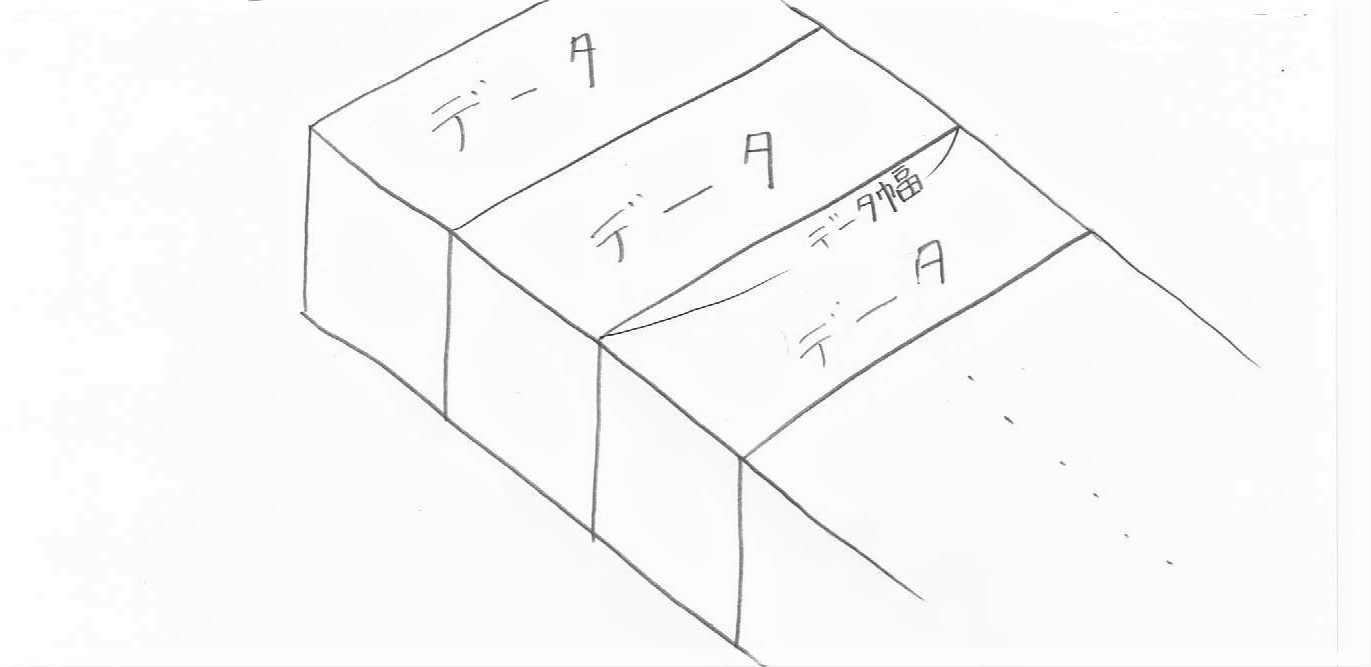
\includegraphics[height=4.5cm]{honda/image/1.jpeg}
\end{figure}
このように棚がズラーっと並んでいるだけなのである。それぞれの棚のなかにはもちろん0,1のデータが入っている。図1のデータ幅というのはこの一つの棚に何個のデータが入るかということで、パソコンなどに使われるメモリは一つの棚にデータが8個入るものが多い。\\
\begin{figure}[H]
  \centering
  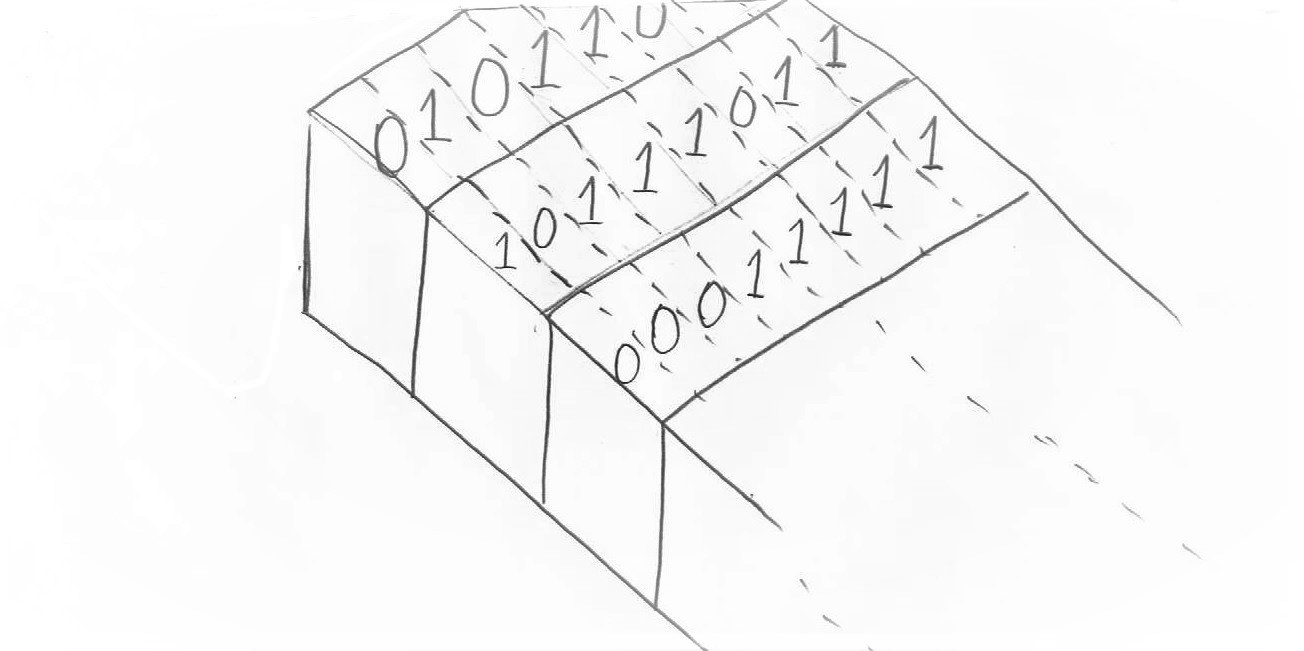
\includegraphics[height=4.5cm]{honda/image/2.jpg}
\end{figure}
この0,1のデータ一つを1bitと呼び、8bitはひとまとめで1Byte(1B)と呼ばれる。\\ 
\begin{figure}[H]
  \centering
  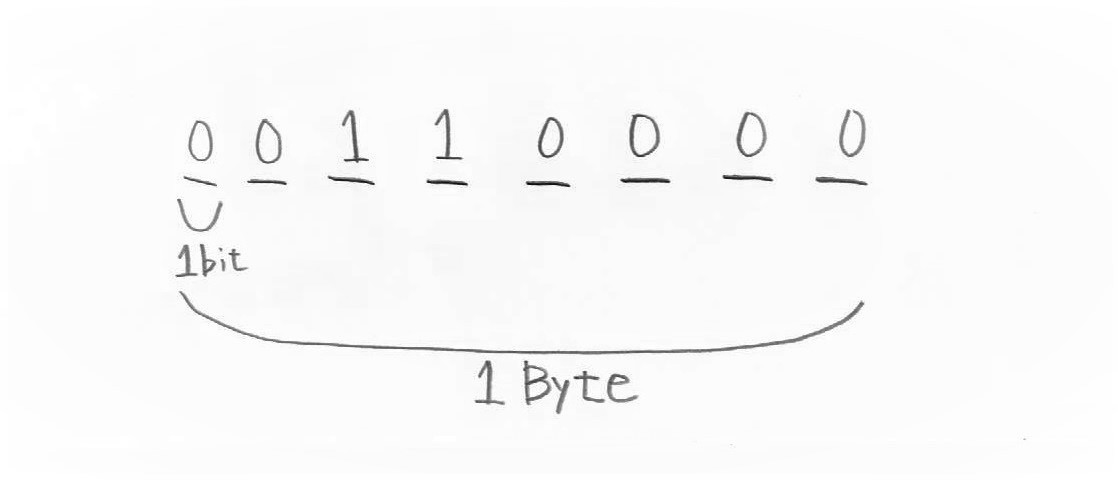
\includegraphics[height=3cm]{honda/image/3.jpeg}
\end{figure}
次にメモリを理解するうえで最も重要な概念、「アドレス」について説明する。アドレスとは英語で「住所」という意味がある。メモリで使うアドレスという言葉も「住所」と同じような使い方をする。先ほど説明した8個のデータが入っている棚一つ一つにそれぞれ番号が振り当てられており、その番号のことをアドレスと呼んでいるのである。
\begin{figure}[H]
  \centering
  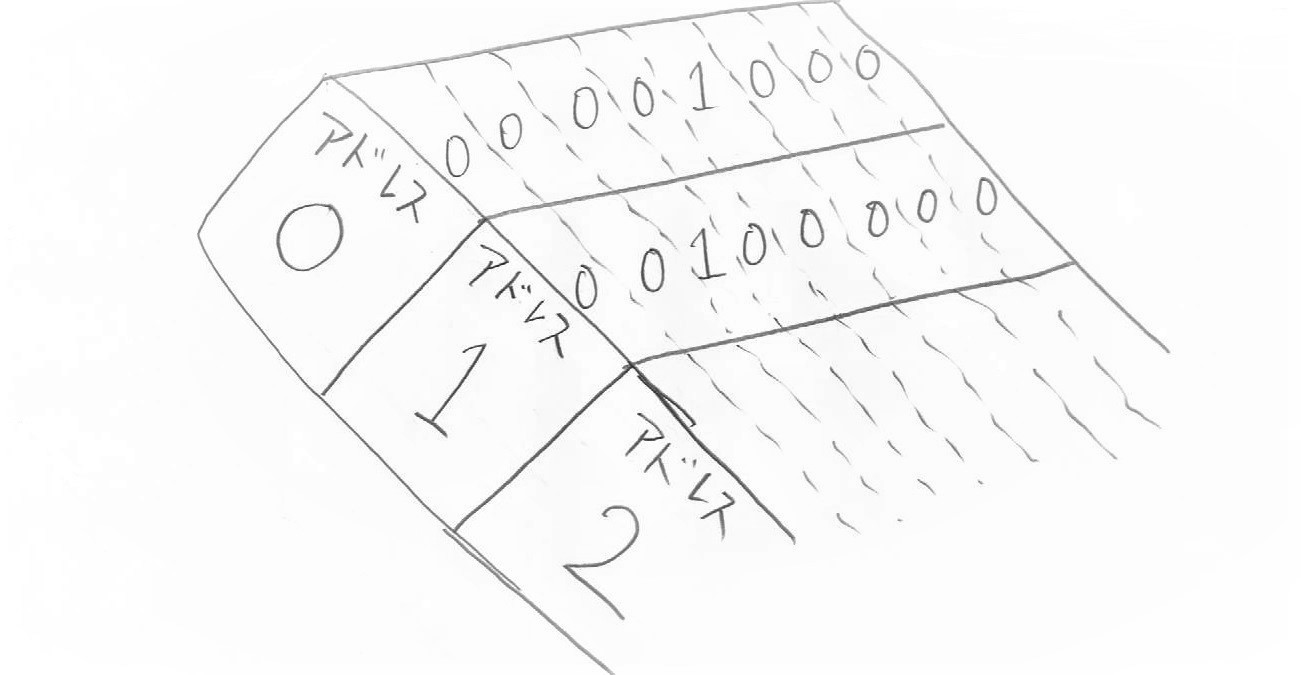
\includegraphics[height=4.5cm]{honda/image/4.jpg}
\end{figure}
上の図ではアドレスを10進数で表したが、実際はコンピュータが扱いやすいように二進数で表現される。また、下図の二進数の0の数はメモリのサイズ(棚の数)によって変わる。
\begin{figure}[H]
  \centering
  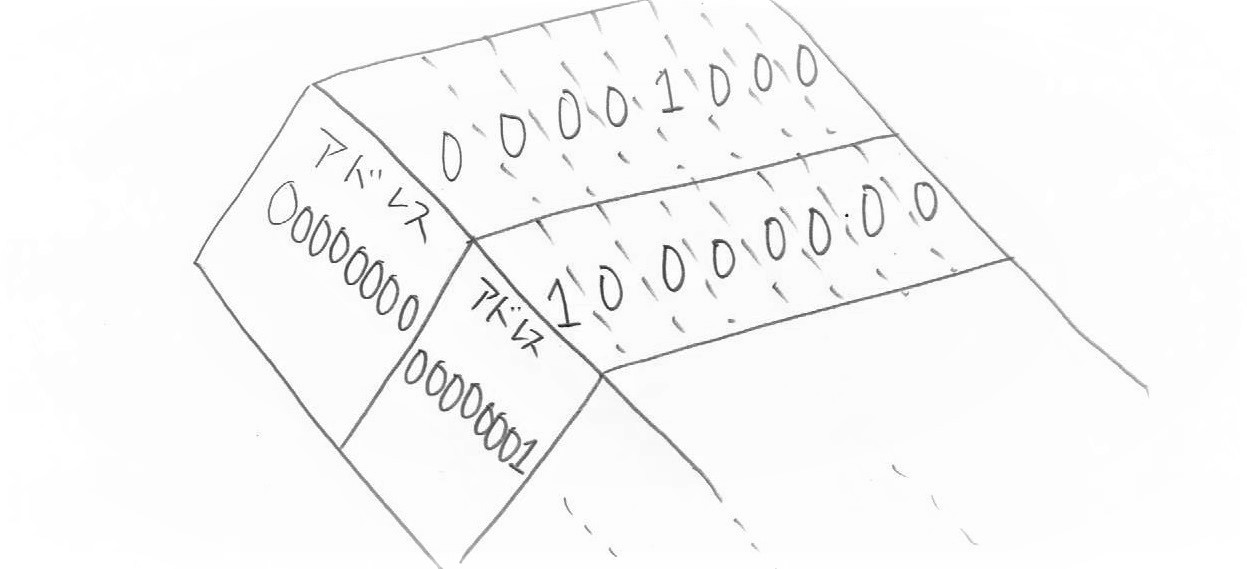
\includegraphics[height=4.5cm]{honda/image/5.jpg}
\end{figure}
大まかなメモリの構造についての説明はこれで終わりで、ここからはより具体的にメモリについて説明する。\\
RAM,ROMについて \\
メモリには大きく分けてRAM,ROMの二種類がある。どちらも構造は先ほど説明した棚のようなものにアドレスが振られているのだが、ROMとRAMでは何が違うのか。\\
ROM…Read Only Memory\\
RAM…Random Access Memory\\
ROM,RAMの略称はこのようになるのだが、これだけ見てもどちらがどのような機能なのかはわからない。ROMとRAMの違いを簡単に説明するなら、「電源を切ったときにデータが消えてしまうか、残ったままか」ということころである。ROMもRAMも電気で動く部品なので、当然動かすには電源が必要である。電源を入れることによってはじめてメモリの中を見たり、書き換えたりできるのである。そして、重要なのはこの電源を「切ったとき」である。ROMの場合それまで入っていたデータが電源を切っても残り続け、次に電源を入れたときは前回のデータのままになっている。\\
\begin{figure}[H]
  \centering
  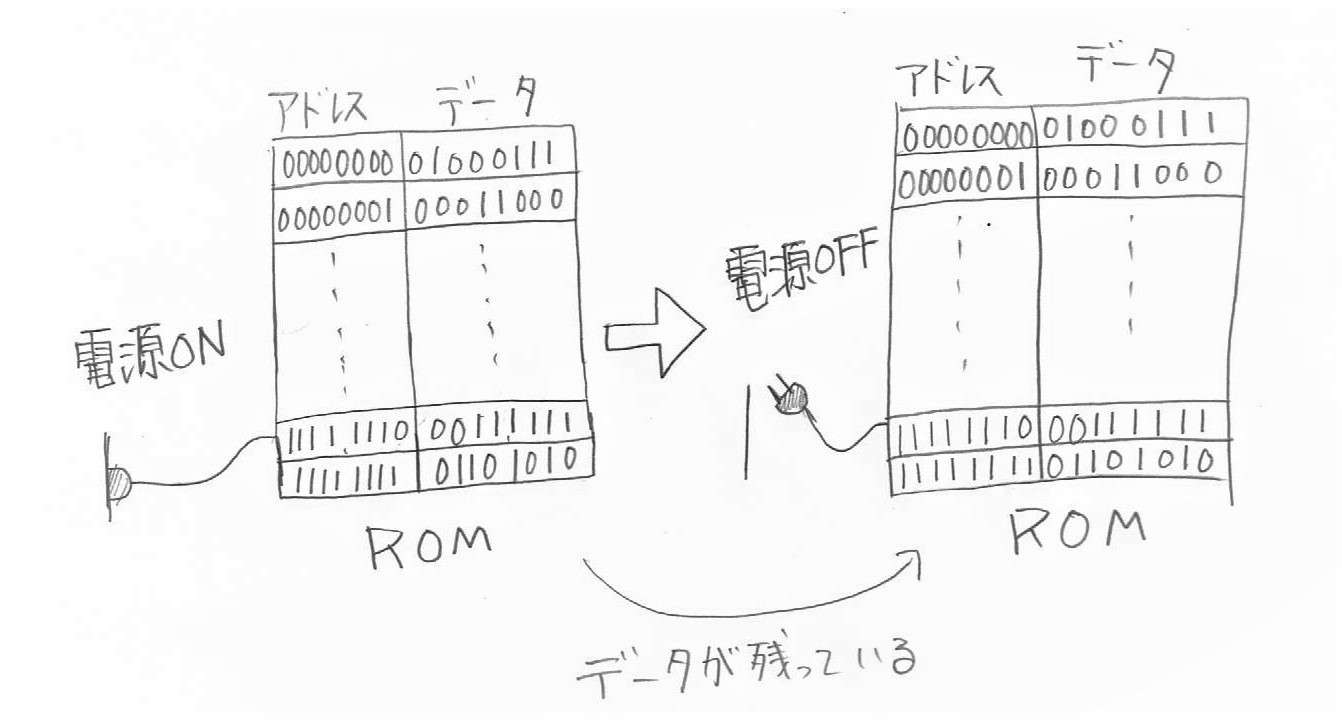
\includegraphics[height=7cm]{honda/image/6.jpeg}
\end{figure}
RAMの場合は1度電源を切ると、それまで入っていたデータは消えてなくなってしまう。では、もう一度電源を入れたときにメモリの中身はどうなっているのか?一度電源を切ってもう一度入れなおしたとき、RAMの中身は全くでたらめな値が入っている。
\begin{figure}[H]
  \centering
  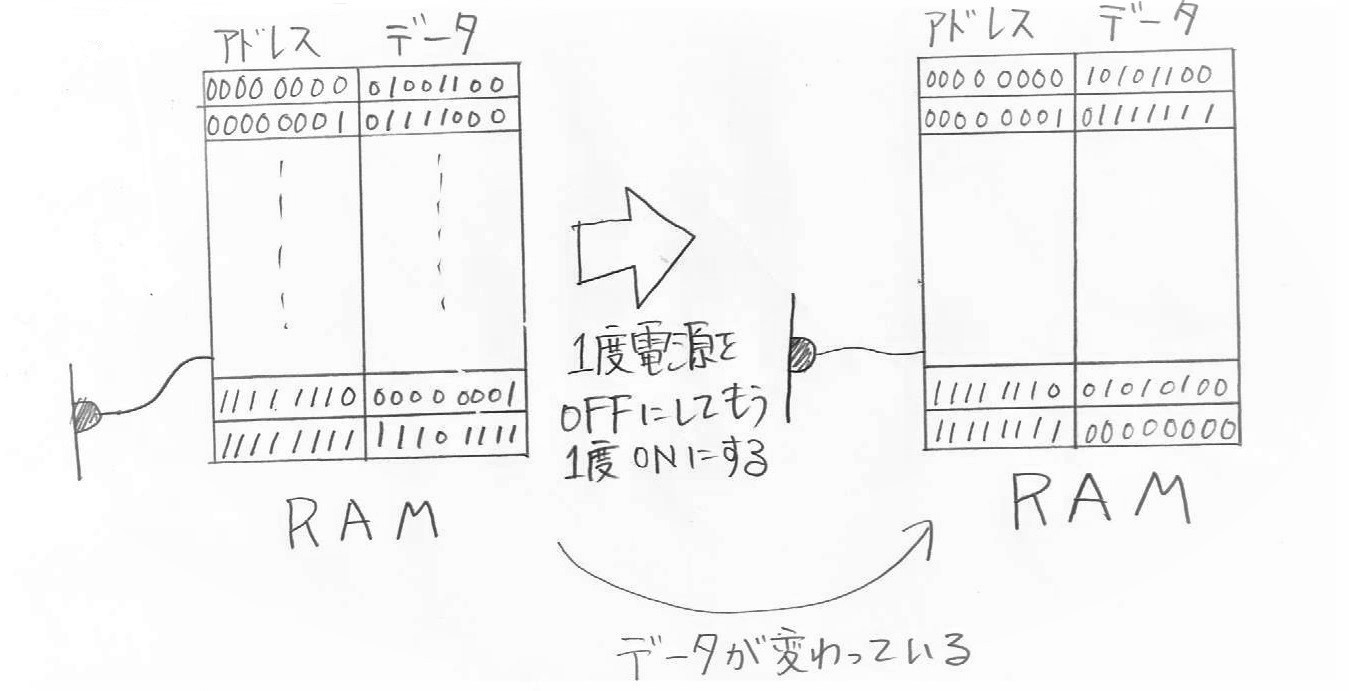
\includegraphics[height=7cm]{honda/image/7.jpg}
\end{figure}
これだけ聞くとRAMよりもROMのほうが役に立ちそうな気もするが、RAM,ROMそれぞれにメリット、デメリットがあり、適材適所に使用される。例を上げればROMはUSBメモリやHDDなどに使われ、RAMはパソコンのスペックを言い表すときに使われる「メモリ」という部分に使われている。\\

\section{レジスタ}
次に、レジスタについて説明する。レジスタというと今まで一度も聞いたことがないという人もいるだろう。簡単に説明するとレジスタもメモリの一種であり、RAMである。では、なぜレジスタという名前を付けて読んでいるのか、それは、CPUの内部にもともと入っている特殊なRAMだからである。ここで初めてCPUの内部の話が出てきたが、CPUの構造について概要を理解してもらうために簡単な概略図を次に示す。\\
\begin{figure}[H]
  \centering
  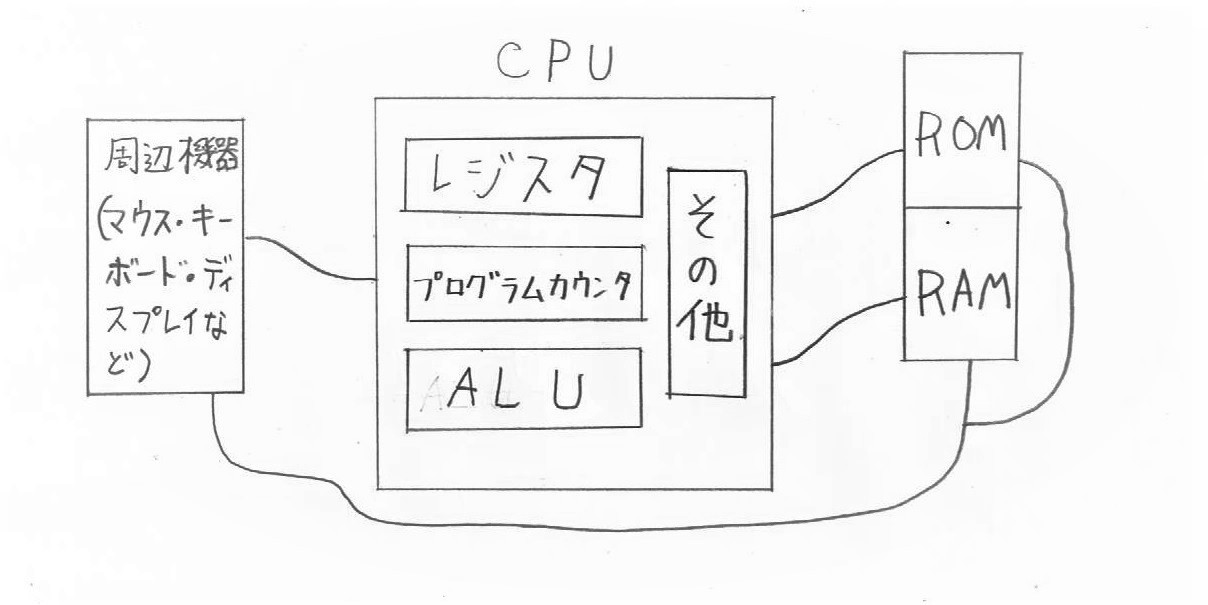
\includegraphics[height=5cm]{honda/image/8.jpeg}
\end{figure}
レジスタは機能的にはほとんどRAMだと思っていい。レジスタの使用例も交えて次の章から改めて解説していく。

\section{機械語}
CPUを動かすためにはCPUにこちらから命令を送らなければならない。CPUは0か1しか取り扱えないので、送る命令は00010110111とか00011111111みたいな命令になってしまう。これを機械語命令というのだが、こんなの人間に理解できるはずがないと思うかもしれない。しかし、そんなこともない。というのも、最新のcore i7~みたいな高機能なCPUならさすがに途方もない量の資料を読み込まないと理解できないとは思うが、まだ動作が単純な頃の古いCPUの機械語なんかだと、それほど苦労することなく理解できたりする。そして、その古いCPUよりもさらに単純な構造で、CPUについてあまり知らない人にもわかりやすいように作られた「自作CPU」というものがある。自作CPUについて書いている本は書店で購入することができ、初心者にとっては非常にとっつきやすいものになっている。今回は、その自作CPUレベルで使用される機械語を使っていくつかのCPUの処理を解説する。
\begin{align*}
0000,0101,0001,0000
\end{align*}
唐突だが、この命令は「内部レジスタに0001,0000を書きこむ」という命令である。もう少し詳しく説明すると、この命令は次のようなブロックに分けて説明することができる。
\begin{figure}[H]
  \centering
  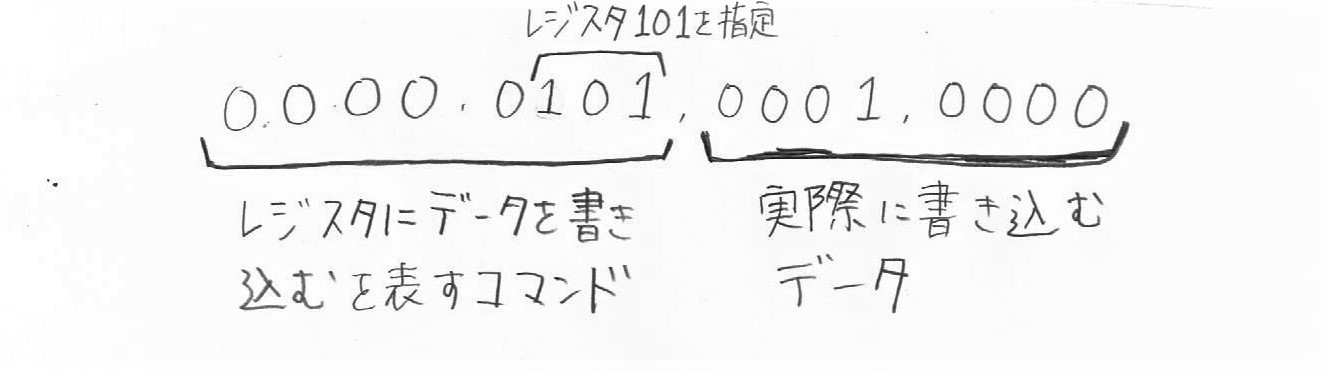
\includegraphics[height=2cm]{honda/image/9.jpg}
\end{figure}
ここで一つ注意してほしいのは、0000,0101が「レジスタにデータを書き込む」という命令を表すといっているが、なにも0000,0101である必要は全くない。今回はわかりやすくするためにこのようにしているが、実際はCPUの回路設計者が決めることである。回路設計者によって0000,0000が「レジスタにデータを書き込む」を意味することもあるし、0000だけで「レジスタにデータを書き込む」を表す場合だってある。その場合、0101が入っていた部分はどうするのかと思うかもしれないが、それも回路設計者によるもので、そこになにが入っても関係ないようなCPUもあれば、そこを細かい追加設定用に使用するCPUもある。しかし、これはあくまで自作CPUレベルの機械語の話であって、実際に使われているCPUはこんなに簡単な話では済まない。\\
ここで、少し話を変えて、レジスタについて説明する。先ほどレジスタについてほとんどRAMと同じだが、少し違うところもあるといったが、その違いは「メモリの数」である。メモリは棚のようなものがずらーっと並んでおり、その一つ一つにアドレスが振られていると言ったが、自作CPUの規模になるとレジスタは数個しかない。つまり、1Byteのデータが入る棚が数個しか並んでないのである。\\
\begin{figure}[H]
  \centering
  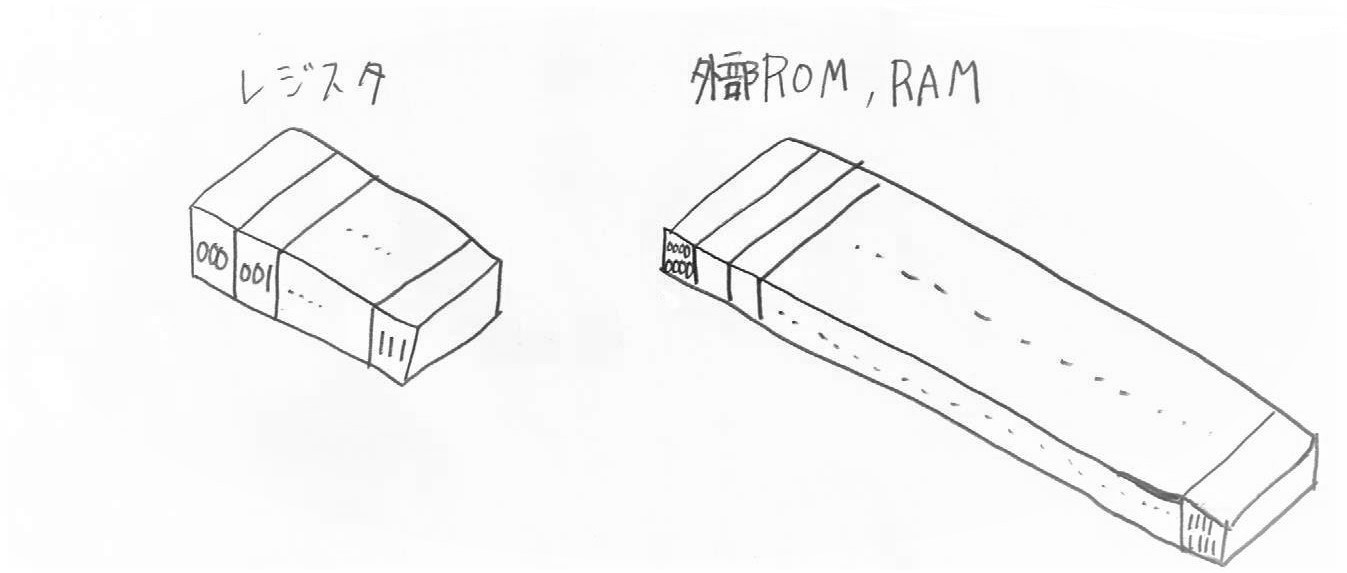
\includegraphics[height=3cm]{honda/image/10.jpg}
\end{figure}
なので、先ほどの機械語ではレジスタ選択に3bitのデータを使っていたので、000~111までの8個のレジスタがあるということになる(実際にレジスタが何個入っているかはCPUによって違う)\\
 先ほどの例と同様にほかの機械語も説明していく。ただし、回路設計上で決める命令の割り当て方についてはあらかじめこちらで決めたものを使うことにし、今回はこのような命令があるということの紹介だけを行うものとする。
\begin{enumerate}
  \item メモリのn番地にレジスタの値を書き込む
  \begin{figure}[H]
    \centering
    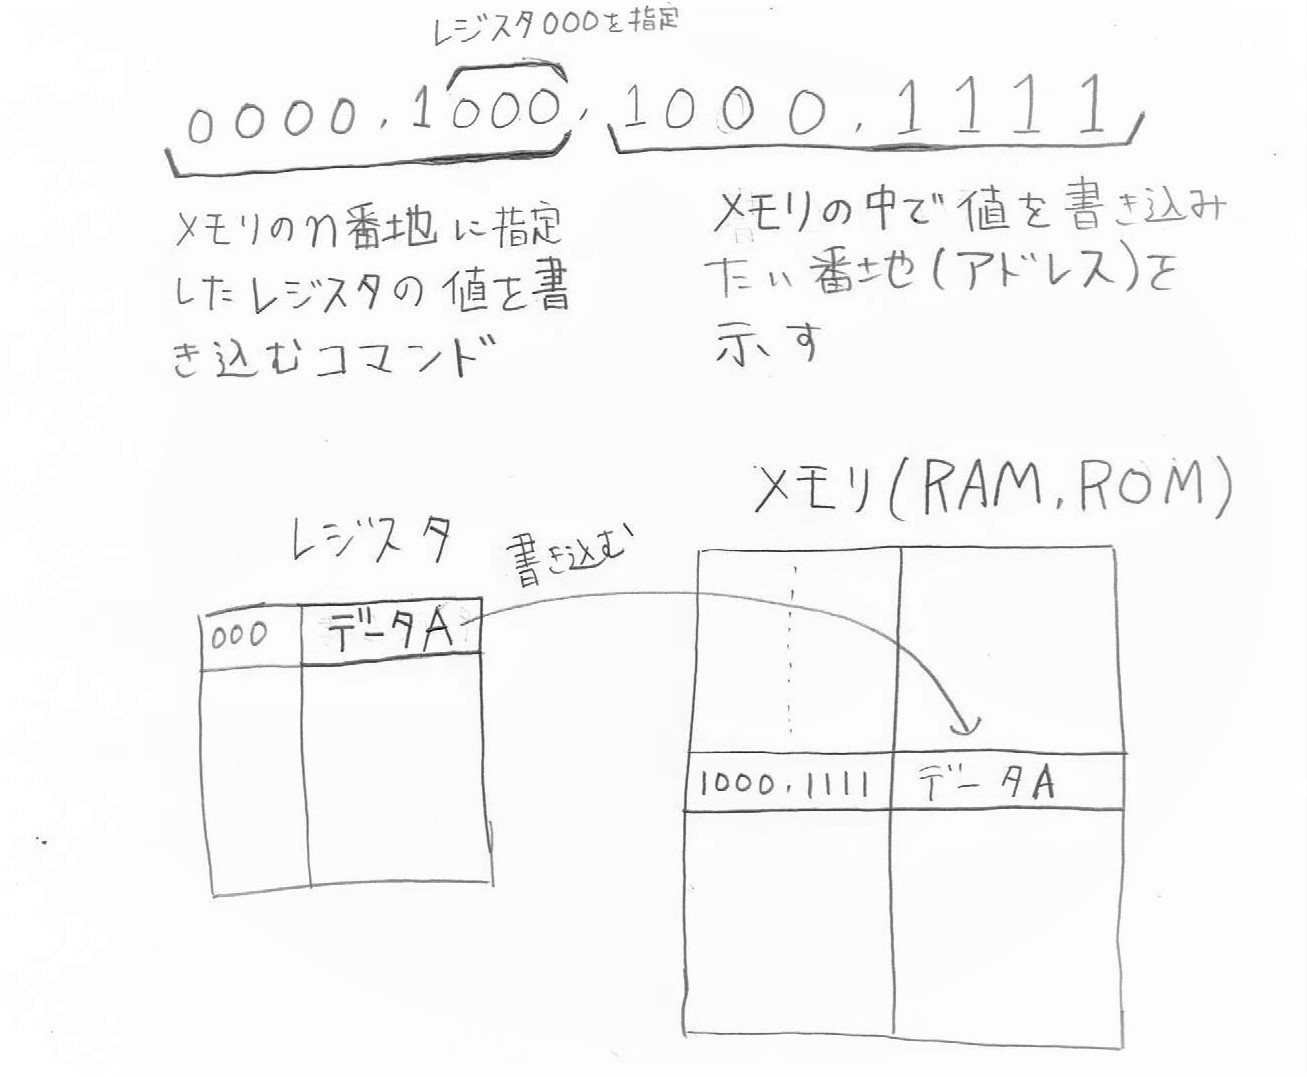
\includegraphics[height=6cm]{honda/image/12.jpg}
  \end{figure}
  この命令を先ほどのレジスタにデータを書き込む命令と一緒に使えば、メモリの好きな場所に好きなデータを書き込むことができる
  \item	メモリのn番地のデータをレジスタに読み出す
  \begin{figure}[H]
    \centering
    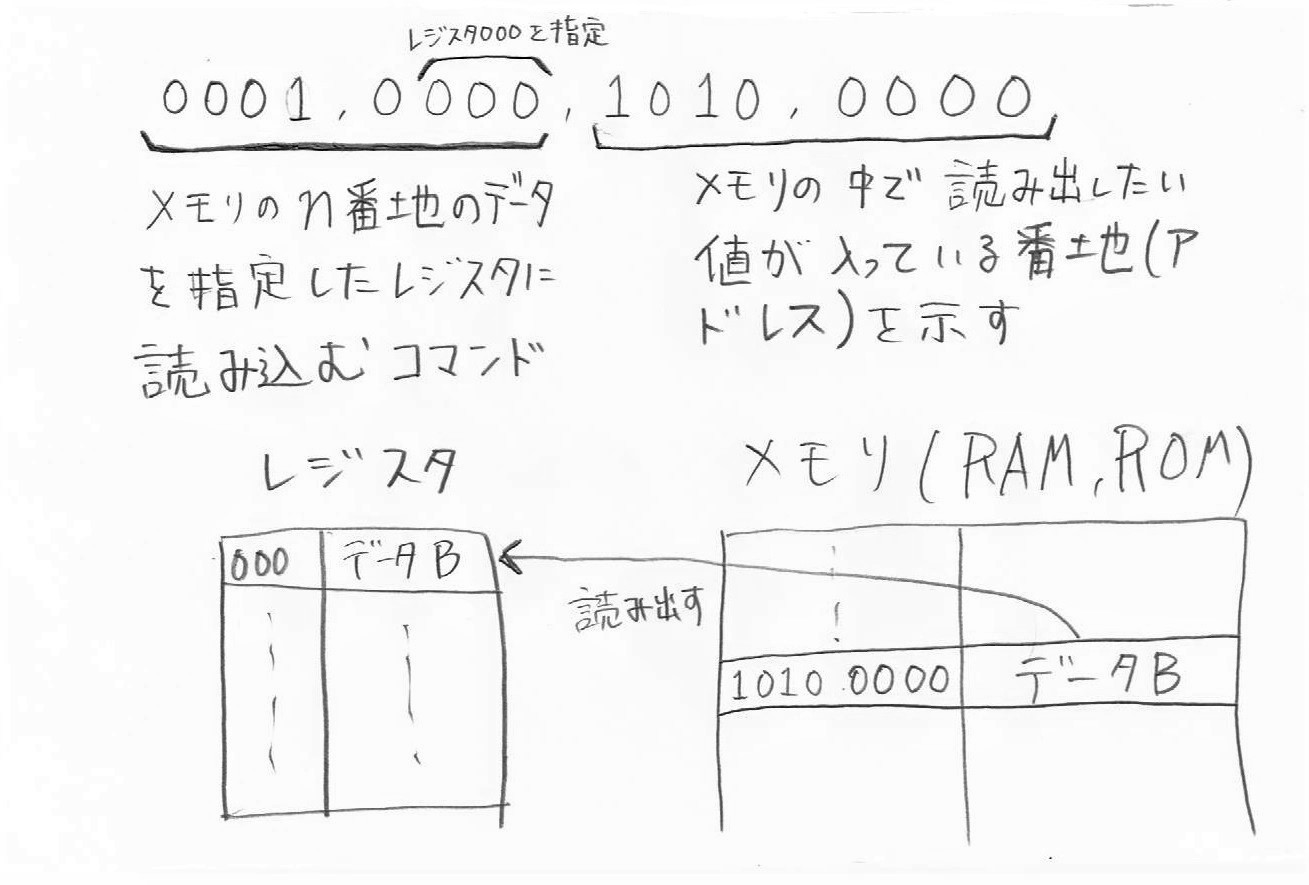
\includegraphics[height=6cm]{honda/image/13.jpg}
  \end{figure}
  この命令でメモリ上のどのデータでも確認することができる
  \item レジスタの値に任意のデータを足し算する
  \begin{figure}[H]
    \centering
    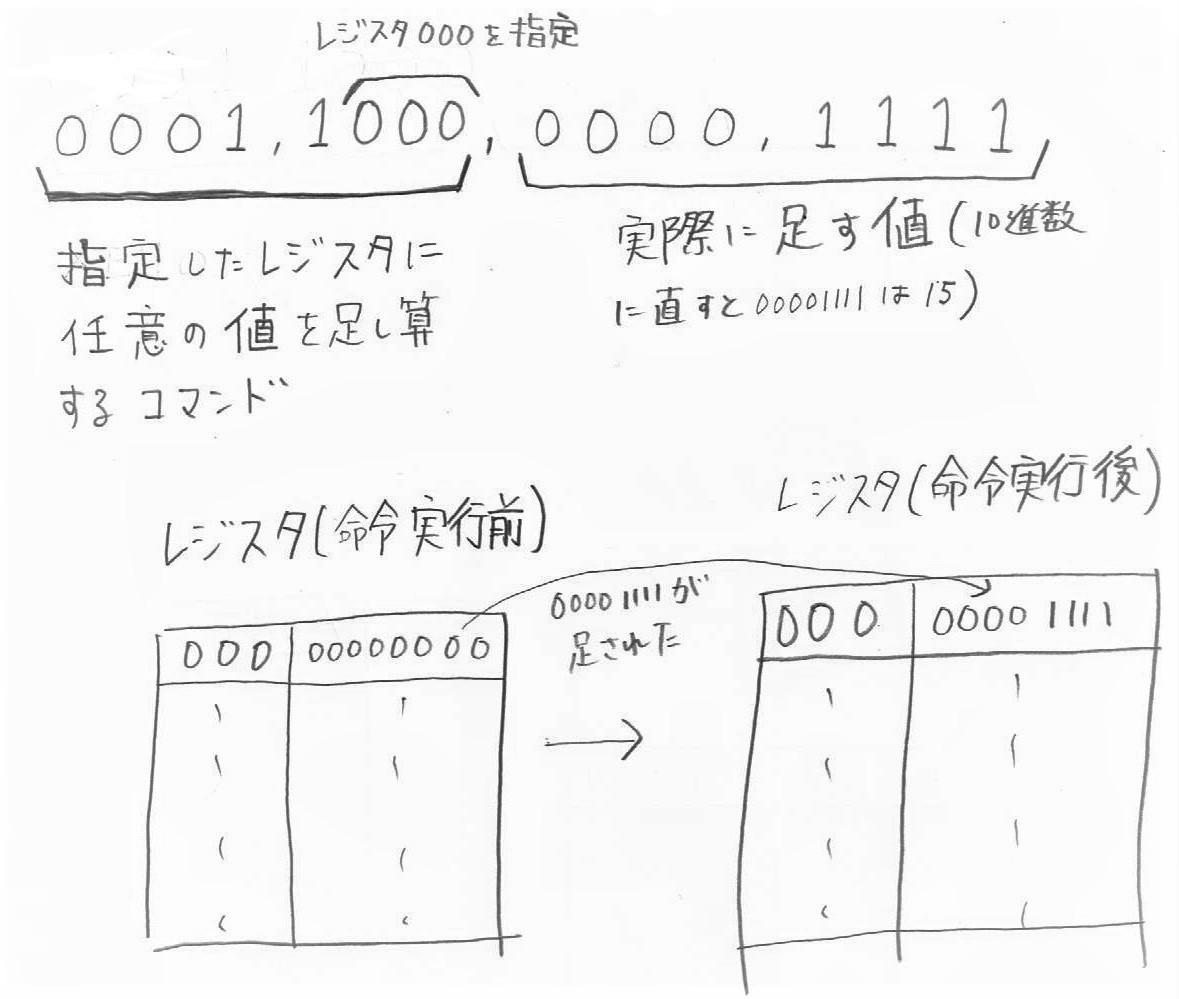
\includegraphics[height=6cm]{honda/image/11.jpg}
  \end{figure}
  引き算も用意されており、掛け算や割り算は足し算、引き算を繰り返すことで実装する。
\end{enumerate}
これだけでは漠然としていてなにができるのかよくわからないかもしれないが、これらの命令を使用するうえで重要なプログラムカウンタという概念について次に説明する。
\section{プログラムカウンタ}
先ほど説明した命令はCPUの命令のうちほんの少しの部分ではあるが、それでもデータの書き込み、読み出し、足し算や引き算などはできる。しかし、これだけだと電卓と機能はほとんど変わらない。では、CPU特有の機能とは何だろうか。それは「何もしなくても命令を順番に実行してくれること」である。先ほどの説明の通り、CPUで扱う命令は0と1のデータである、ということは、メモリの中に保存することができる。なので、CPUを動かすための命令のデータはすべてメモリの中に書き込まれているのである。\\
ここで、「CPUはいったいどこの命令から実行していくのか」と疑問に思ったひとがいると思う。それを決めるのがCPUのプログラムカウンタという部分だ。プログラムカウンタが何をしているかといえば、簡単に説明すると、「メモリの中のどのアドレスの部分の命令を実行するかを指し示すもの」である。ずらーっと並んでいる棚の中から、どれか2つ(今回説明で使った機械語は16bitのデータなので、今回は棚2つ分)が命令として使われる。そのどれかを示しているのがプログラムカウンタなのだが、このプログラムカウンタの賢いところが、命令が一つ実行されるたびに現在の値から1命令分(今回だと棚2つ分)値が増えるのだ。こうすることによってずっと同じ命令を繰り返すのではなく、次から次へと命令を順番に実行していくことができる。またプログラムカウンタは電源を入れた直後は0を示しており、メモリの一番初めに入っている命令を実行することになる。電卓の場合、0を入力、1を足すなどの命令を実行するのにわざわざ指でボタンを押さないといけない。しかし、CPUの場合、メモリの上からレジスタに0を書き込む、1を足すなどの命令を入れておけばいちいちボタンを押さなくても勝手に順番に実行していってくれるし、1秒間に100や1000もの命令を実行することができるので、大量の命令を瞬時にこなすことができ、電卓とは比べ物にならない性能を持っていることがわかる。\\
\begin{figure}[H]
  \centering
  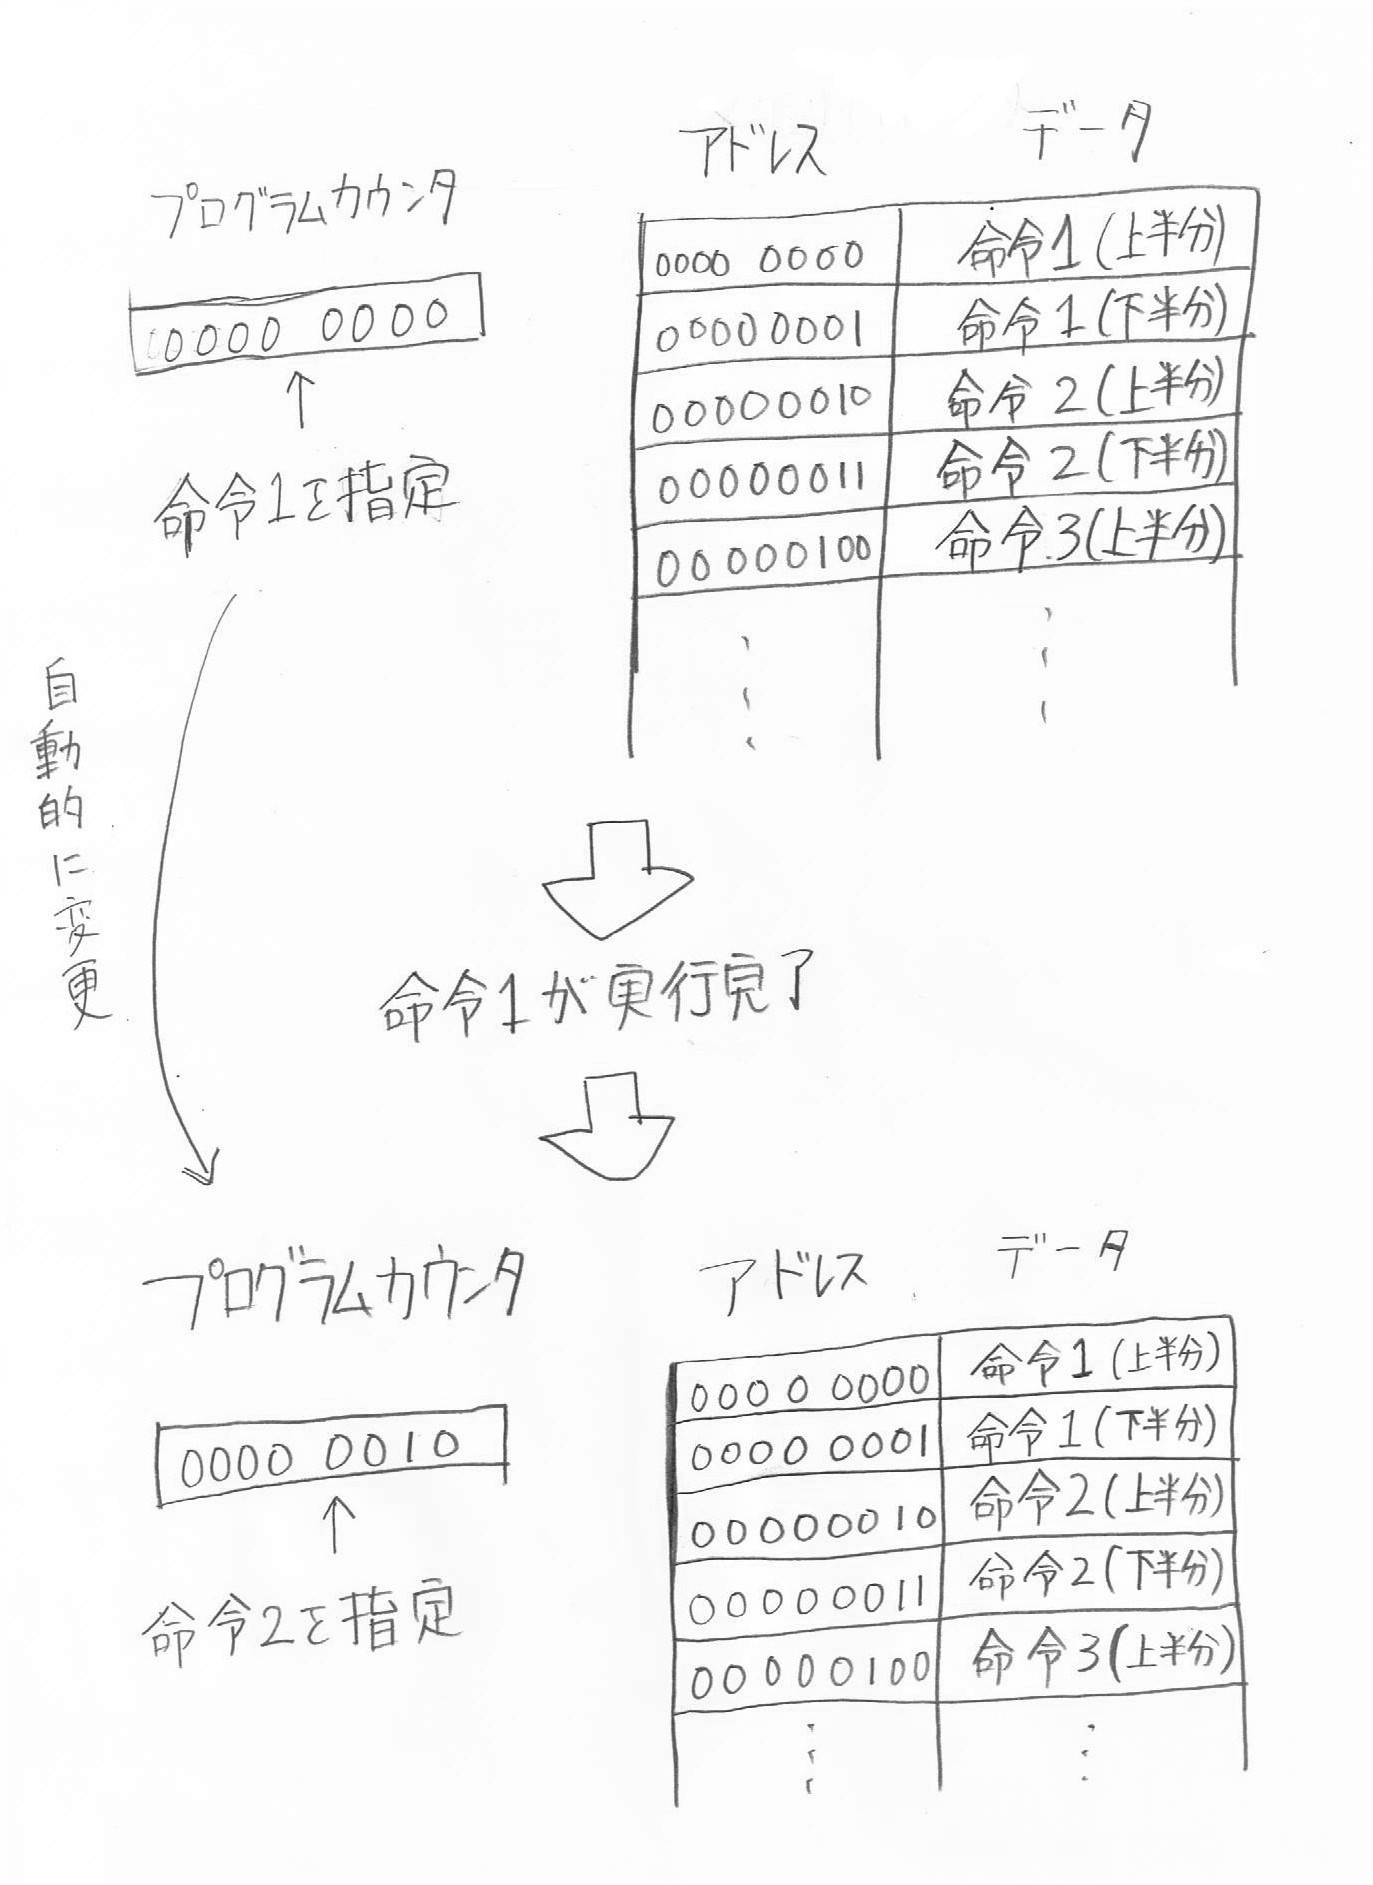
\includegraphics[height=7cm]{honda/image/14.jpg}
\end{figure}
\section{まとめ}
ここまでCPUについていろいろ解説してきたが、これだけではCPUを使えばosを動かしたり、ゲームをしたり、動画を見れたりすることの説明には全くならない。そのようなことはもっといろいろな知識がないと理解できない。しかし、今回私が伝えたかったのはCPUの動作の中でも一番基本の「CPUとメモリの関係」の部分であり、これを理解しているのとしていないのではCPUに対する理解度はかなり違うと思う。これまでCPUが何をしているのかなどまったく気にしたことがなかった人にも、少しCPUについて分かった気になってもらえたらうれしい。\\


%参考文献
%thebibliographyは使わないでください。\chapterになっちゃう!
\section*{参考文献}
\begin{enumerate}
  \item 渡波郁著,CPUの作り方
\end{enumerate}
 \clearpage


%
\backmatter %以降章番号を付けない。


%
\chapter*{編集後記}
\addcontentsline{toc}{chapter}{あとがき}
編集を担当しました中山です。これを書いているのは学園祭前日です。つまりギリギリでした。会誌提出の締め切りは1ヶ月延長することとなりましたが、一応形にはしてきてくれたのでなんとか完成させることができました。みなさんお疲れ様でした。\par
去年の学園祭では会誌はとりあえず手書きでもWordでもなんでもいいから各自作ってもらい、それを1つにつなげるだけというものでした。しかしそれでは通しでページ番号を付けられないという問題が発生し、次からはみんな\TeX で書きましょうということになりました。今年のOB会で去年の会誌を全部\TeX で作り直し、かなりきれいにできたので今回も表紙以外は\TeX で作りました。\par
表紙と裏表紙は、会長最後の仕事として門野先輩に作っていただきました。今までお疲れ様でした。学園祭を期に、会長は2回生の西村君に交代です。頑張ってください。
 \vspace{3mm}\\
{\bf P.S. \,\,部員へ}\par
来年度はみっちり\TeX 講座を行います。
\begin{flushright}
  2017年11月25日\\
  物理科学科 2回生 中山 敦貴
\end{flushright}

\vspace{8zw} \hrulefill \par
{\large \bf 2017年度 物理科学研究会会誌}\par
\quad 2017年11月26日 発行

\end{document}
